%%
%% LaTeX Document Template
%%
\documentclass[sigplan,screen]{acmart}
%%
%% \BibTeX command to typeset BibTeX logo in the docs
\AtBeginDocument{%
  \providecommand\BibTeX{{%
    Bib\TeX}}}

%% Publication information - modify as needed
\setcopyright{acmlicensed}
\copyrightyear{2024}
\acmYear{2024}
\acmDOI{XXXXXXX.XXXXXXX}
\acmConference[]{University of Auckland}{University of Auckland}{2025}
\acmISBN{978-1-4503-XXXX-X/2024/XX}

%% Citation style configuration
\citestyle{acmauthoryear}


%%
%% Additional packages for figures and subfigures
\usepackage{graphicx}
\usepackage{subcaption}

%%
%% Hyperref is automatically loaded by acmart class
%% Configure colors for links
\hypersetup{
    colorlinks=true,
    linkcolor=blue,
    citecolor=red,
    urlcolor=cyan
}

%%
%% end of the preamble, start of the body of the document source.
% Improve line breaking to avoid overfull boxes for long words
\emergencystretch=3em
\begin{document}

%%
%% The "title" command has an optional parameter,
%% allowing the author to define a "short title" to be used in page headers.
\title[Data Mining]{ A Fraud Detection Solution for Extremely Imbalanced Financial Data}

%% Author information
\author{Xiaoqing Miao}
\email{xmia665@aucklanduni.ac.nz}
\affiliation{%
  \institution{University of Auckland }
  \city{Auckland}
  \country{New Zealand}
}


%% Short author list for page headers
\renewcommand{\shortauthors}{Xiaoqing Miao}

%%
%% The abstract is a short summary of the work to be presented in the
%% article.
\begin{abstract}
\sloppy
In Iteration-3, our primary objective is minimizing expected cost under a business loss ratio of FP:FN = 1:25. We select the operating threshold from a validation-set cost--threshold curve and evaluate on the original-distribution test set. Using the PaySim dataset, we focus on TRANSFER/CASH\_OUT transactions, apply log1p transformation + standardization, compare down-sampling LR (Iter-A) versus class-weighted LR (Iter-B), and adopt Iter-B as the current operating candidate.

On the test set, the model achieves ROC-AUC = 0.9756 (meeting the project-level AUC target of $\geq$0.95) and PR-AUC(AP) = 0.582. At the recommended operating point $\tau$ = 0.9488, we obtain Precision = 27.42\%, Recall = 65.95\%, and FPR = 0.52\%, delivering the lowest expected cost among candidates. This operating point does not yet satisfy the project-level stretch targets Precision $\geq$ 70\% / Recall $\geq$ 85\%; thus, we position it as a cost-optimal baseline and outline next steps: targeted feature engineering and non-linear models (e.g., stronger tree-based learners and interaction terms), tighter threshold--alert quota coupling, and entity/time-grouped robustness checks. Overall, Iteration-3 secures strong ranking performance and a reproducible cost--recall trade-off, establishing a clear path to reach the project's stretch goals.
\fussy
\end{abstract}

%% CCS concepts and keywords - add your own
%% Generate CCS concepts at: https://dl.acm.org/ccs/ccs.cfm
%%\begin{CCSXML}
%%...your CCS XML here...
%%\end{CCSXML}
%%\ccsdesc[500]{Your primary concept}
%%\ccsdesc[300]{Your secondary concept}

%% Keywords
\keywords{fraud detection, class imbalance, CRISP-DM, logistic regression, PaySim dataset}

%% Optional teaser figure
%%\begin{teaserfigure}
%%  \includegraphics[width=\textwidth]{your-image}
%%  \caption{Your teaser figure caption.}
%%  \Description{Description of your teaser figure.}
%%  \label{fig:teaser}
%%\end{teaserfigure}

%% Submission dates (optional)
%%\received{Date}
%%\received[revised]{Date}
%%\received[accepted]{Date}

%%
%% This command processes the author and affiliation and title
%% information and builds the first part of the formatted document.
\maketitle

\section{Business/Situation Understanding}
\subsection{Business/Situation Objectives}

\textbf{Business Context}

The digital payment industry is facing severe fraud challenges. The PaySim dataset simulates one month of mobile payment transactions, containing a total of 6,362,620 records, of which only 0.13\% (8,213 transactions) are fraudulent, reflecting the highly imbalanced nature of real-world scenarios.

\textbf{Key Business Objectives}

\begin{itemize}
\item \textbf{Reduce Financial Losses:} Reduce fraud-related losses by 75\% through early detection.
\item \textbf{Protect Customer Trust:} Prevent customers from becoming fraud victims and maintain customer satisfaction above 90\%.
\item \textbf{Optimize Operational Efficiency:} Reduce manual fraud investigation workload by 60\%.
\end{itemize}

\textbf{Business Success Criteria}

\begin{itemize}
\item \textbf{Detection Performance:} Recall $\geq$ 85\%, Precision $\geq$ 70\%, AUC score $\geq$ 0.95.
\item \textbf{Operational Efficiency:} Transaction processing time < 100 milliseconds, system availability $\geq$ 99.9\%.
\item \textbf{Financial Impact:} ROI of 10:1 (for every \$1 invested, prevent \$10 in fraud losses).
\end{itemize}

\textbf{Two-level Goals and Binding (Iteration-3 $\leftrightarrow$ \S8.4)}\newline
\begin{itemize}
\item \textbf{Iteration Goal (Iteration-3)}: Min Cost @ FP:FN=1:25 \textbf{(Achieved)}. Operating threshold $\tau_B{=}0.9488$ selected via validation-set cost--threshold curve under operational constraints (theoretical basis in \citealp{elkan2001foundations}); all evaluation in Chapter 8 follows this $\tau_B$.
\item \textbf{Project-level Hard Targets}: AUC $\geq$ 0.95 \textbf{(Achieved, 0.9756)}; Precision $\geq$ 70\% / Recall $\geq$ 85\% \textbf{(Not achieved)}. This iteration serves as the cost-optimal baseline for subsequent improvements.
\end{itemize}

\textbf{Alignment with Data Mining Objectives}

These business objectives directly translate to:

\begin{itemize}
\item Building a binary classifier for fraud detection (fraud vs. legitimate).
\item Identifying high-risk patterns in TRANSFER and CASH\_OUT transactions.
\item Developing real-time risk scoring for transaction approval decisions.
\end{itemize}

\textbf{Expected Value}

Through fraud prevention and control, annual savings of \$300,000--\$750,000 can be achieved, reducing investigation costs by \$75,000, and enhancing market competitive positioning as a secure payment platform.

\subsection{Assessment of the Situation}

\subsubsection{Resource Inventory}
As an individual student project, available resources include: PaySim open-source dataset (6.36 million transaction records), personal laptop (16GB RAM), Anaconda Python environment with Jupyter Notebook (with installed libraries including NumPy, Pandas, Matplotlib, Seaborn, scikit-learn, etc.), and 2 weeks of project time. Knowledge resources include course materials, Kaggle dataset documentation, online tutorials, and relevant academic papers. As a data mining course student, I possess foundational knowledge of classification algorithms and operational experience with Python data analysis and modeling tools.

\subsubsection{Requirements and Assumptions}
\textbf{Requirements}: Complete all phases of CRISP-DM, build a binary classification model capable of detecting fraudulent transactions with a performance target of AUC $\geq$ 0.95, and submit a comprehensive project report covering data understanding, modeling process, and results interpretation.

\textbf{Assumptions}: PaySim synthetic data adequately reflects real-world fraud characteristics; personal laptop (16GB RAM) can handle \textbf{6,362,620} transaction records; two-week project cycle is sufficient for multiple iterations; Python and Jupyter Notebook with common data analysis libraries (such as Pandas, scikit-learn) have the functionality to meet project requirements.

\subsubsection{Constraints}

\begin{itemize}
\item \textbf{Time Constraints}: Project must be completed within 2 weeks, with 15-20 hours available per week.
\item \textbf{Technical Constraints}: Limited by personal computer's computational performance (16GB RAM), may require data sampling or batch processing.
\item \textbf{Data Constraints}: Can only rely on publicly available PaySim synthetic dataset, lacking real business transaction data for further validation (PaySim simulator: \citealp{paysim2016emss}).
\item \textbf{Experience Constraints}: As a student, limited experience in actual business operations and risk control processes for financial fraud detection.
\end{itemize}

\subsubsection{Risks and Mitigation Measures}
Project risk assessment covers five main risk areas: technical, performance, time, software, and data. For each risk, specific response plans are developed to ensure the project can be completed successfully under adverse conditions, thereby maximizing the possibility of achieving project objectives.

\begin{center}
\textbf{Risk Assessment Table}
\end{center}

\begin{table}[h!]
    \centering
\tiny
\renewcommand{\arraystretch}{1.3}
\begin{tabular}{|p{1.0cm}|p{2.0cm}|p{0.8cm}|p{0.8cm}|p{2.9cm}|}
\hline
\textbf{Risk Category} & \textbf{Risk Description} & \textbf{Prob.} & \textbf{Impact} & \textbf{Mitigation Measures} \\
\hline
Technical & Limited memory may cause bottlenecks processing 6.36M records & Med. & High & 1. Stratified sampling\newline 2. Batch processing\newline 3. Use lab computers \\[2pt]
\hline
Performance & Model may not reach AUC $\geq$ 0.95 target & Med. & High & 1. Multiple algorithms\newline 2. Ensemble methods\newline 3. Feature engineering \\[2pt]
\hline
Time & 2-week timeframe insufficient for complete iterations & Med. & Med. & 1. Prioritize core phases\newline 2. Optional optimization\newline 3. Daily milestones \\[2pt]
\hline
Software & Python environment or dependency conflicts & Low & High & 1. Virtual environments\newline 2. Regular saves\newline 3. Google Colab backup \\[2pt]
\hline
Data & Extreme imbalance (fraud only 0.13\%) causes majority bias & High & Med. & 1. SMOTE oversampling\newline 2. Class weights\newline 3. Precision-recall tuning \\[2pt]
\hline
\end{tabular}
\caption{Project Risk Assessment and Mitigation Strategies}
\label{tab:risk_assessment}
\end{table}

See Table \ref{tab:risk_assessment} for the project's risk assessment and mitigation strategies.

\subsection{Data Mining Objectives}
    
The primary objective of this project is to \textbf{build an effective classification model to accurately predict the isFraud label in financial transactions}. Specifically, it aims to distinguish between normal transactions (isFraud = 0) and fraudulent ones (isFraud = 1) by analyzing various transaction features (e.g., transaction type, amount, account balance changes).
    
\subsubsection{Model Evaluation Methods}
    
Due to the significantly smaller number of fraud samples compared to normal samples, the dataset exhibits severe class imbalance. Therefore, the traditional \textbf{Accuracy metric is misleading} and will not be used as the primary evaluation criterion.

Instead, this study adopts the \textbf{ROC Curve (Receiver Operating Characteristic Curve)} and its \textbf{Area Under the Curve (AUC)} as the core evaluation metric. AUC measures the model's overall ability to distinguish between positive and negative samples, is insensitive to class imbalance, and is widely recognized as a reliable standard for addressing such problems.
    
\subsubsection{Success Criteria}
    
To ensure data mining outcomes directly serve business objectives, I have established the following clear, quantifiable technical success criteria. The model's final performance will be evaluated on an independent test set using these metrics:

\begin{enumerate}
\item \textbf{Overall Discrimination Ability (AUC - Area Under Curve):}
\begin{itemize}
    \item \textbf{Standard:} AUC $\geq$ 0.95
    \item \textbf{Rationale:} AUC is the gold standard for measuring a model's overall ability to distinguish between positive and negative samples (fraud vs. normal), especially when dealing with imbalanced data. Setting a high standard of 0.95 aims to ensure we obtain a model with excellent discriminative capability.
\end{itemize}
\item \textbf{Fraud Capture Capability (Recall):}
    \begin{itemize}
    \item \textbf{Standard:} Recall $\geq$ 85\%
    \item \textbf{Rationale:} This is the \textbf{most critical business metric} for this project. High recall means the model can successfully identify the vast majority (at least 85\%) of actual fraudulent transactions. This directly corresponds to the core business objective of ``reducing financial losses,'' as missing a genuine fraud (False Negative) is extremely costly.
    \end{itemize}
\item \textbf{Prediction Accuracy (Precision):}
\begin{itemize}
    \item \textbf{Standard:} Precision $\geq$ 70\%
    \item \textbf{Rationale:} While ensuring high recall, we also need to control the false positive rate. High precision means when the model raises an alarm, there's a high probability (at least 70\%) it's actually fraud. This directly relates to the business objective of ``optimizing operational efficiency,'' effectively reducing time and costs wasted by investigators on normal transactions (False Positives).
\end{itemize}
\end{enumerate}
    
A model is considered successful only when it meets or exceeds all three key performance metrics simultaneously. This multidimensional evaluation system ensures our technical solution is not only statistically effective but also meets business value standards.
    
\subsubsection{Model Interpretation and Deployment}
    
The scope of this analysis is strictly limited to modeling and validation in this iteration; \textit{adopting comprehensive evaluation using ROC-AUC and PR-AUC (with PR preferred under extreme imbalance \citep{saito2015precision}), and under fixed business cost weights FP:FN=1:25, transferring the minimum cost threshold $\tau^*$ from the validation set to the test set, reporting business metrics such as Precision/Recall/FPR/Cost per thousand transactions}. Further business interpretation of model results (such as feature importance analysis) and actual deployment strategies are beyond the scope of this project but will be considered as potential directions for future research.

\subsection{Project Plan}
    
The project plan outlines the main tasks of this project. I have provided a Work Breakdown Structure (WBS) and Gantt chart (see Figure \ref{fig:gantt_chart}) to illustrate the time allocation for each specific task and the iterations between CRISP-DM phases.
    
\textbf{Work Breakdown Structure (WBS)}
    
The following table details the daily task schedule for the project from September 16 to September 25, 2025. This plan has excluded weekends (September 20 and 21) and redistributed the workload accordingly.

\begin{table}[h!]
    \centering
\tiny
\renewcommand{\arraystretch}{1.3}
\begin{tabular}{|p{1.0cm}|p{2.0cm}|p{3.5cm}|p{1.0cm}|}
\hline
\textbf{Date} & \textbf{Core Task} & \textbf{Specific Content} & \textbf{Time} \\
\hline
9/16 & Planning \& Success Criteria & $\bullet$ Review feedback, clarify objectives/success criteria\newline $\bullet$ Develop WBS \& Gantt chart, fix random seeds & 2h \\[2pt]
\hline
9/17 & Data Understanding \& EDA & $\bullet$ Load data \& robustness checks\newline $\bullet$ Visualize distributions \& class imbalance\newline $\bullet$ Screen for leakage risks & 4h \\[2pt]
\hline
9/18 & Data Prep \& Cleaning (1/2) & $\bullet$ Filter transaction types (TRANSFER, CASH\_OUT)\newline $\bullet$ Field trimming \& type conversion\newline $\bullet$ Preprocessing scaffolding & 3h \\[2pt]
\hline
9/19 & Data Prep (2/2) + Imbalance Handling & $\bullet$ Complete cleaning \& finalize features\newline $\bullet$ Implement undersampling \& class\_weight\newline $\bullet$ Establish comparison table & 4.5h \\[2pt]
\hline
9/20-21 & Weekend Buffer & Contingency only (emergency use $\leq$2h/day if necessary) & 0h \\[2pt]
\hline
9/22 & Baseline Model \& Evaluation & $\bullet$ Train/test split\newline $\bullet$ Train LR/tree baseline\newline $\bullet$ Output AUC, PR-AUC, ROC/PR curves\newline (Milestone: Baseline Complete) & 3.5h \\[2pt]
\hline
9/23 & Model Optimization (1/2) & $\bullet$ Standardization \& cross-validation\newline $\bullet$ Compare algorithms (LR vs RF/LightGBM)\newline $\bullet$ Record hyperparameters \& results & 3h \\[2pt]
\hline
9/24 & Model Optimization (2/2) + Documentation (1/2) & $\bullet$ Fine-tuning/finalize threshold\newline $\bullet$ Export charts (confusion matrix, ROC, PR-AUC)\newline $\bullet$ Start writing Methods/Results & 3.5h \\[2pt]
\hline
9/25 & Documentation (2/2) + Paper Revision & $\bullet$ Complete figures \& tables, results interpretation\newline $\bullet$ Full text revision: abstract/conclusion/limitations\newline (Milestone: Report Frozen) & 4.5h \\[2pt]
\hline
9/26 & Final QA \& Submission & $\bullet$ Reproduce experiments (fix seeds, rerun)\newline $\bullet$ Package code \& data, check formatting\newline $\bullet$ Submit & 2h \\[2pt]
\hline
\end{tabular}
\caption{Work Breakdown Structure (WBS) - Daily Task Schedule}
\label{tab:wbs_schedule}
\end{table}

See Table \ref{tab:wbs_schedule} for the WBS daily task schedule.

To provide a more intuitive visualization of the project timeline, task dependencies, and key milestones, I have created the following Gantt Chart. This chart visualizes the tasks from the Work Breakdown Structure (WBS), clearly marking the task arrangements, start and end times, and their interconnections for each working day from September 16 to September 25 (excluding weekends). Through this chart, we can ensure the project progresses in a timely and orderly manner.

\begin{figure*}[h!]
    \centering
    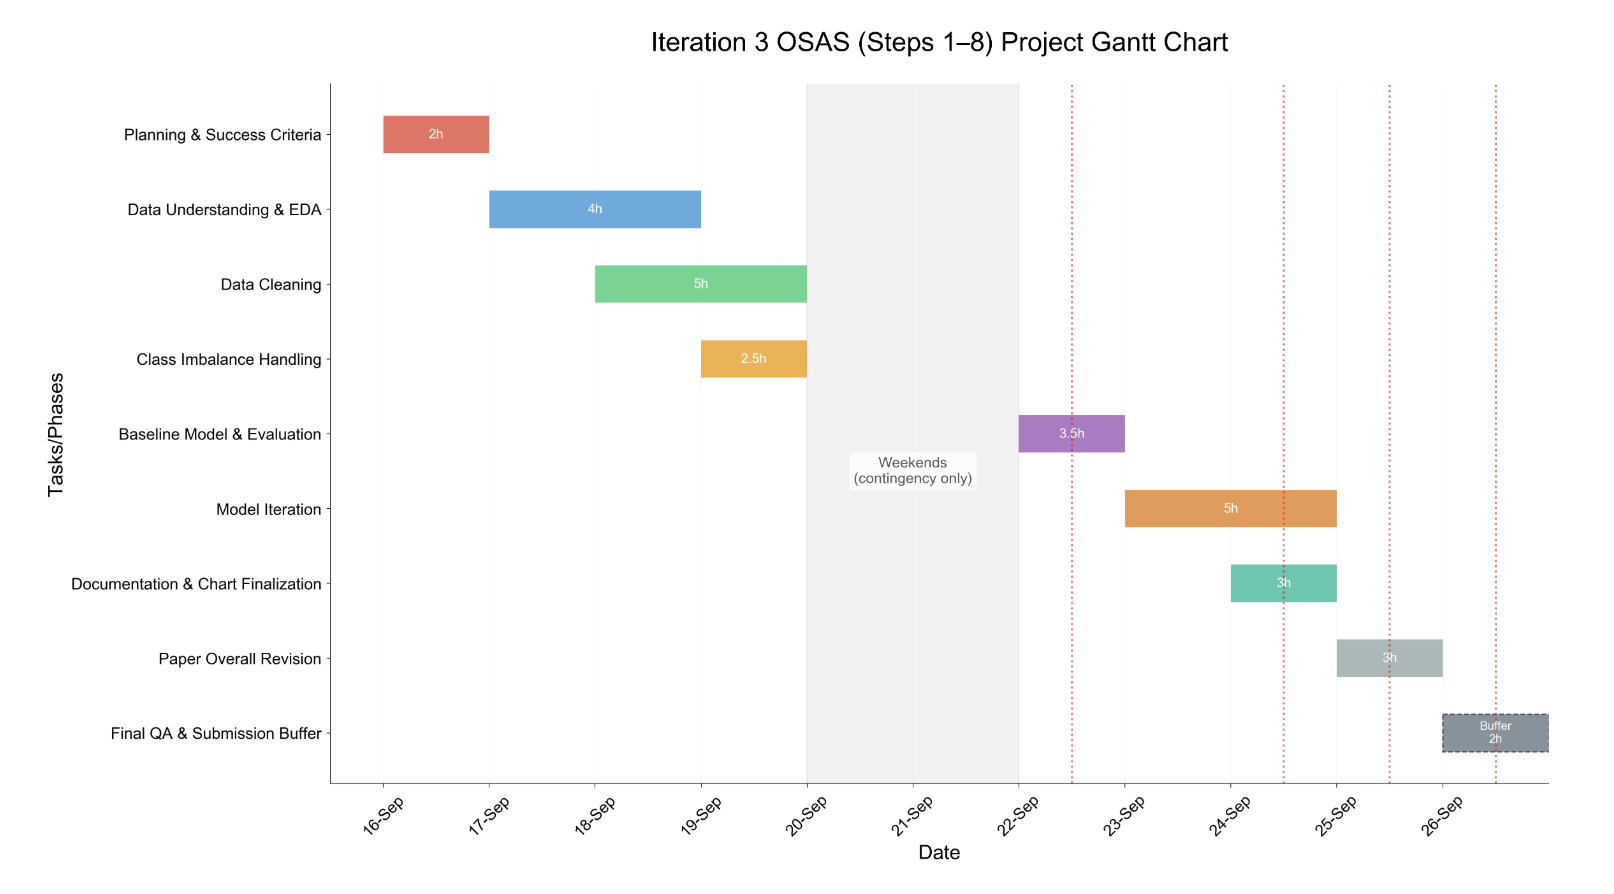
\includegraphics[width=0.9\textwidth]{1.4.png}
    \caption{Iteration 3 OSAS (Steps 1--8) -- Project Gantt Chart (Total: 30h; weekends kept free, used only as contingency)}
    \label{fig:gantt_chart}
\end{figure*}

\section{Data Understanding}
\subsection{Collect Initial Data}

\textbf{Data Source}

The dataset used in this project is \texttt{PaySim}, a publicly available synthetic dataset simulating mobile money transactions, widely used in financial fraud detection research \citep{paysim2016emss}. The original source of this dataset is the Kaggle platform, an authoritative website that provides datasets, programming environments, and community support for data scientists. Data source: \url{https://www.kaggle.com/datasets/ealaxi/paysim1?resource=download}.

\textbf{Data Collection Process}

I downloaded the raw data from the Kaggle platform and saved it as a file named \texttt{Financial Fraud-Rawdata.csv}, stored in the local project path for analysis.

\textbf{Challenges and Solutions in Data Collection}

Since this dataset contains over 6.3 million transaction records with a large file size, traditional spreadsheet software (such as Microsoft Excel) cannot fully load all the data, which posed challenges for preliminary data exploration.

To address this issue, I used Python's \texttt{pandas} library, a powerful data analysis tool capable of efficiently handling large-scale datasets. By executing the \texttt{pd.read\_csv()} function, I successfully read the complete file located at \texttt{data/Financial Fraud-Rawdata.csv} into a DataFrame data structure.

To verify that the data was loaded successfully and correctly, I called the \texttt{.head()} method to preview the first five records of the dataset. The output (see Figure \ref{fig:data_preview}) clearly displays the data headers and structure, confirming the loading process was error-free and establishing a solid foundation for subsequent data analysis work.

\begin{figure}[h!]
    \centering
    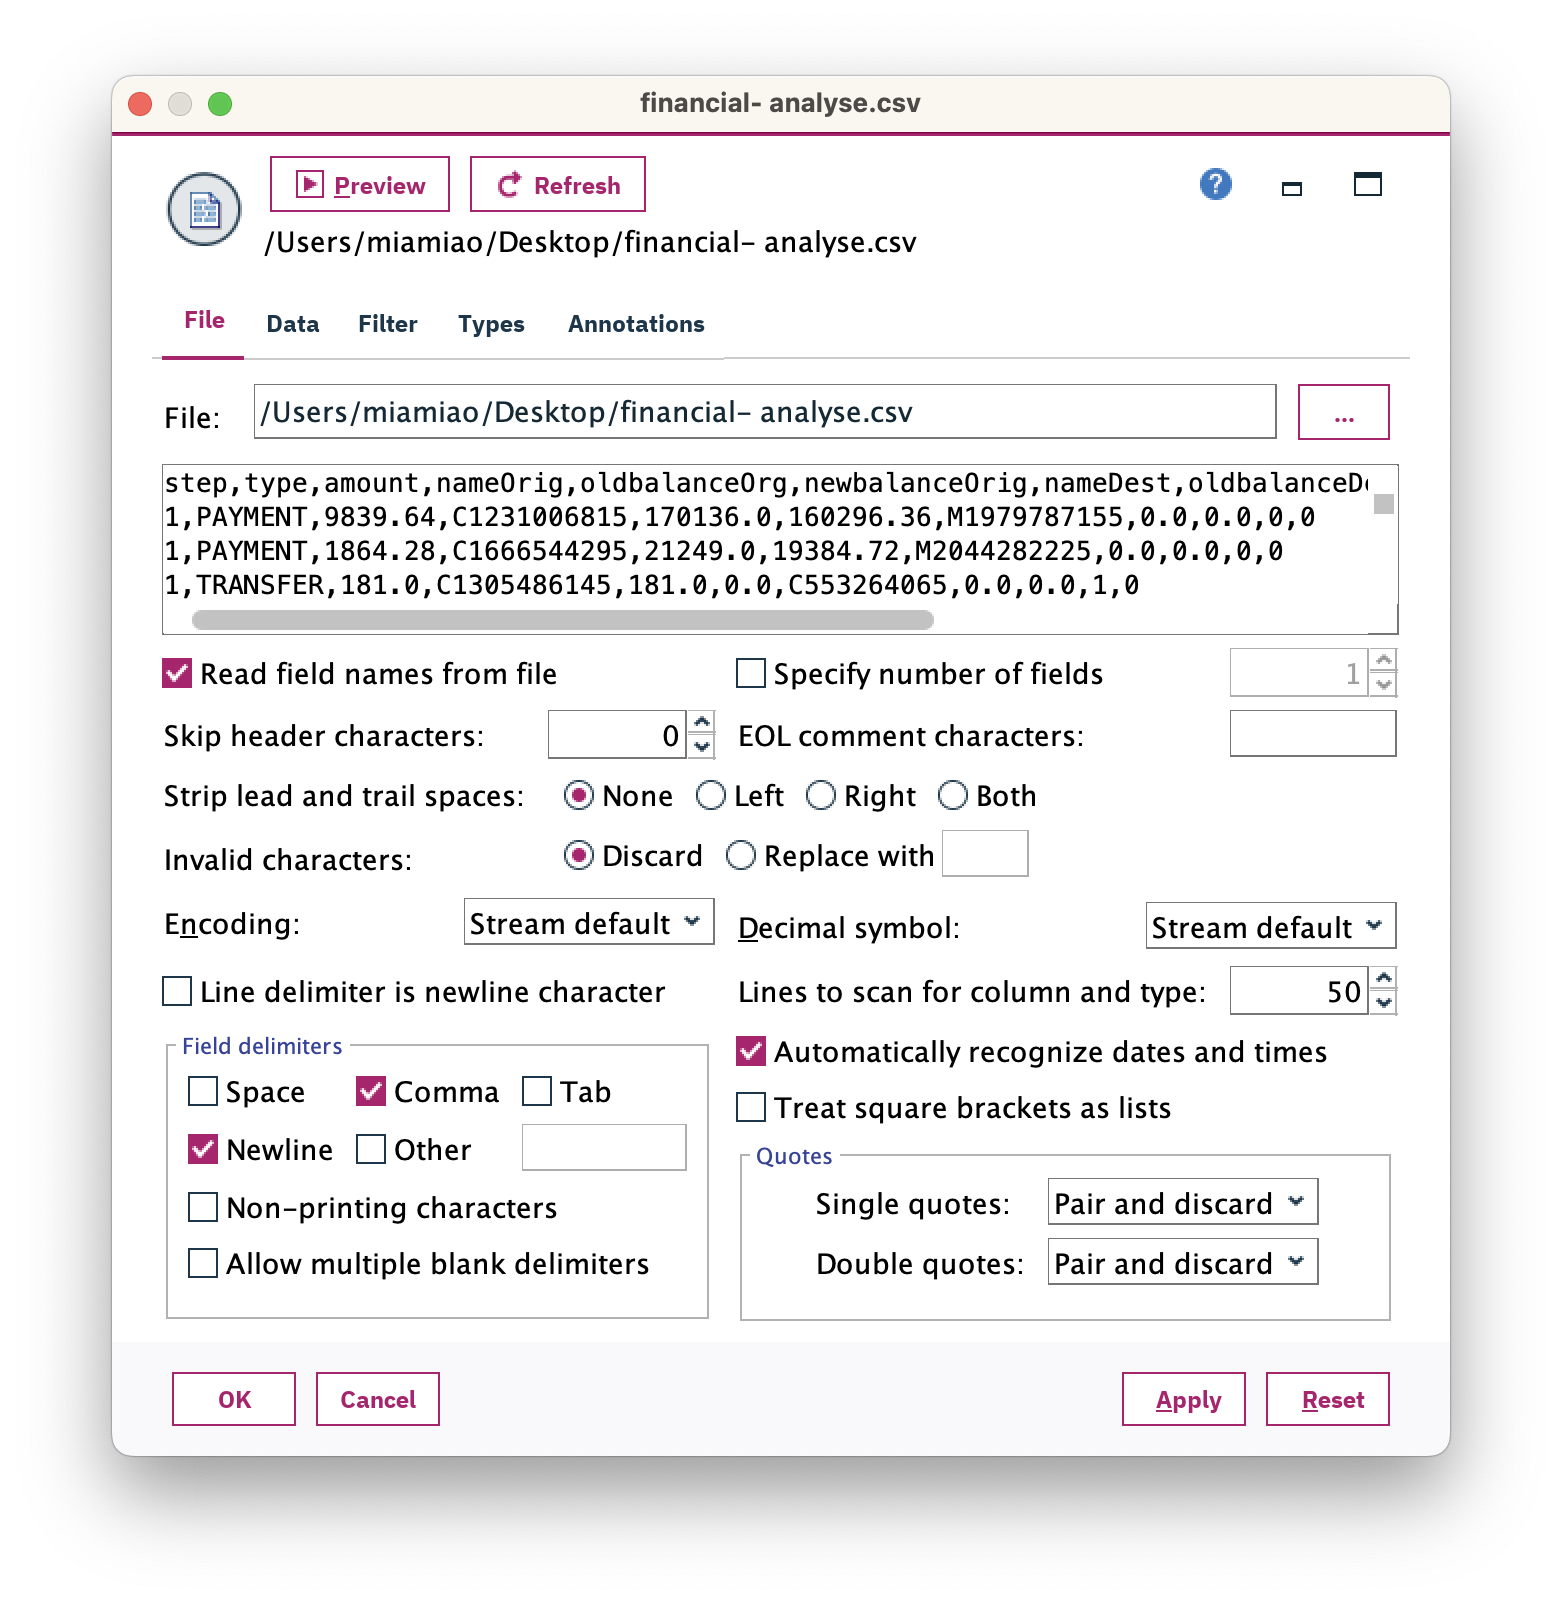
\includegraphics[width=0.9\columnwidth]{2.1.png}
    \caption{Loading and Previewing the Dataset Using Pandas}
    \label{fig:data_preview}
\end{figure}

\subsection{Data Description}

After successfully loading the data, I described the macro structure of the dataset. By calling the \texttt{.info()} method (see Figure \ref{fig:data_info}), I obtained detailed metadata about the dataset.

The dataset is formatted as a \texttt{pandas DataFrame}, containing a total of \textbf{6,362,620} transaction records (rows) and \textbf{11} descriptive fields (columns). The specific fields and their data types are as follows:

\begin{itemize}
\item \textbf{step}: \texttt{int64} (integer), representing time units
\item \textbf{type}: \texttt{object} (object/string), representing transaction type  
\item \textbf{amount}: \texttt{float64} (float), representing transaction amount
\item \textbf{nameOrig / nameDest}: \texttt{object} (object/string), representing transaction party IDs
\item \textbf{oldbalanceOrg / newbalanceOrig}: \texttt{float64} (float), representing originator's balance
\item \textbf{oldbalanceDest / newbalanceDest}: \texttt{float64} (float), representing recipient's balance
\item \textbf{isFraud / isFlaggedFraud}: \texttt{int64} (integer), representing fraud labels
\end{itemize}

A key finding is that all 11 fields have non-null value counts of 6,362,620, which exactly matches the total number of rows in the dataset. This indicates high data quality, with \textbf{no missing values present}, eliminating the need for data imputation. The entire dataset occupies approximately $\approx$534.0+ MB in memory.

\begin{figure}[h!]
    \centering
    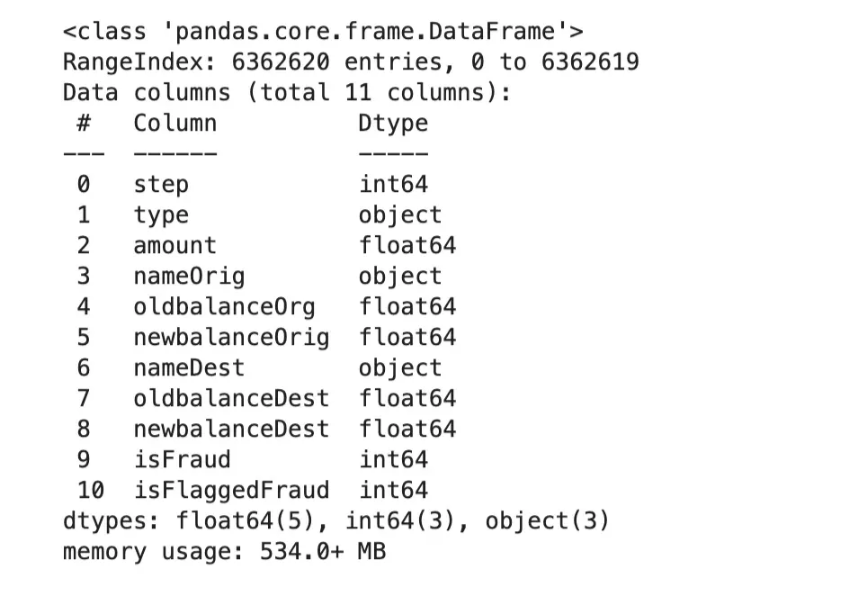
\includegraphics[width=0.9\columnwidth]{2.2.png}
    \caption{Dataset Metadata Overview}
    \label{fig:data_info}
\end{figure}

\subsection{Data Exploration}

In this phase, I conducted Exploratory Data Analysis (EDA) to gain deeper understanding of the patterns and relationships within the data.

First, I performed statistical summary analysis on numerical features. The results showed that the \texttt{amount} (transaction amount) field has an extremely uneven distribution with extreme values, suggesting that a small number of large transactions may have significant impact on the analysis.

To understand the data more intuitively, I conducted visualization analysis. The first step was to explore the distribution of different transaction types (see Figure \ref{fig:transaction_types}). The figure shows that \texttt{CASH\_OUT} and \texttt{PAYMENT} are the two predominant transaction methods, constituting the majority of the dataset.

\begin{figure*}[h!]
    \centering
    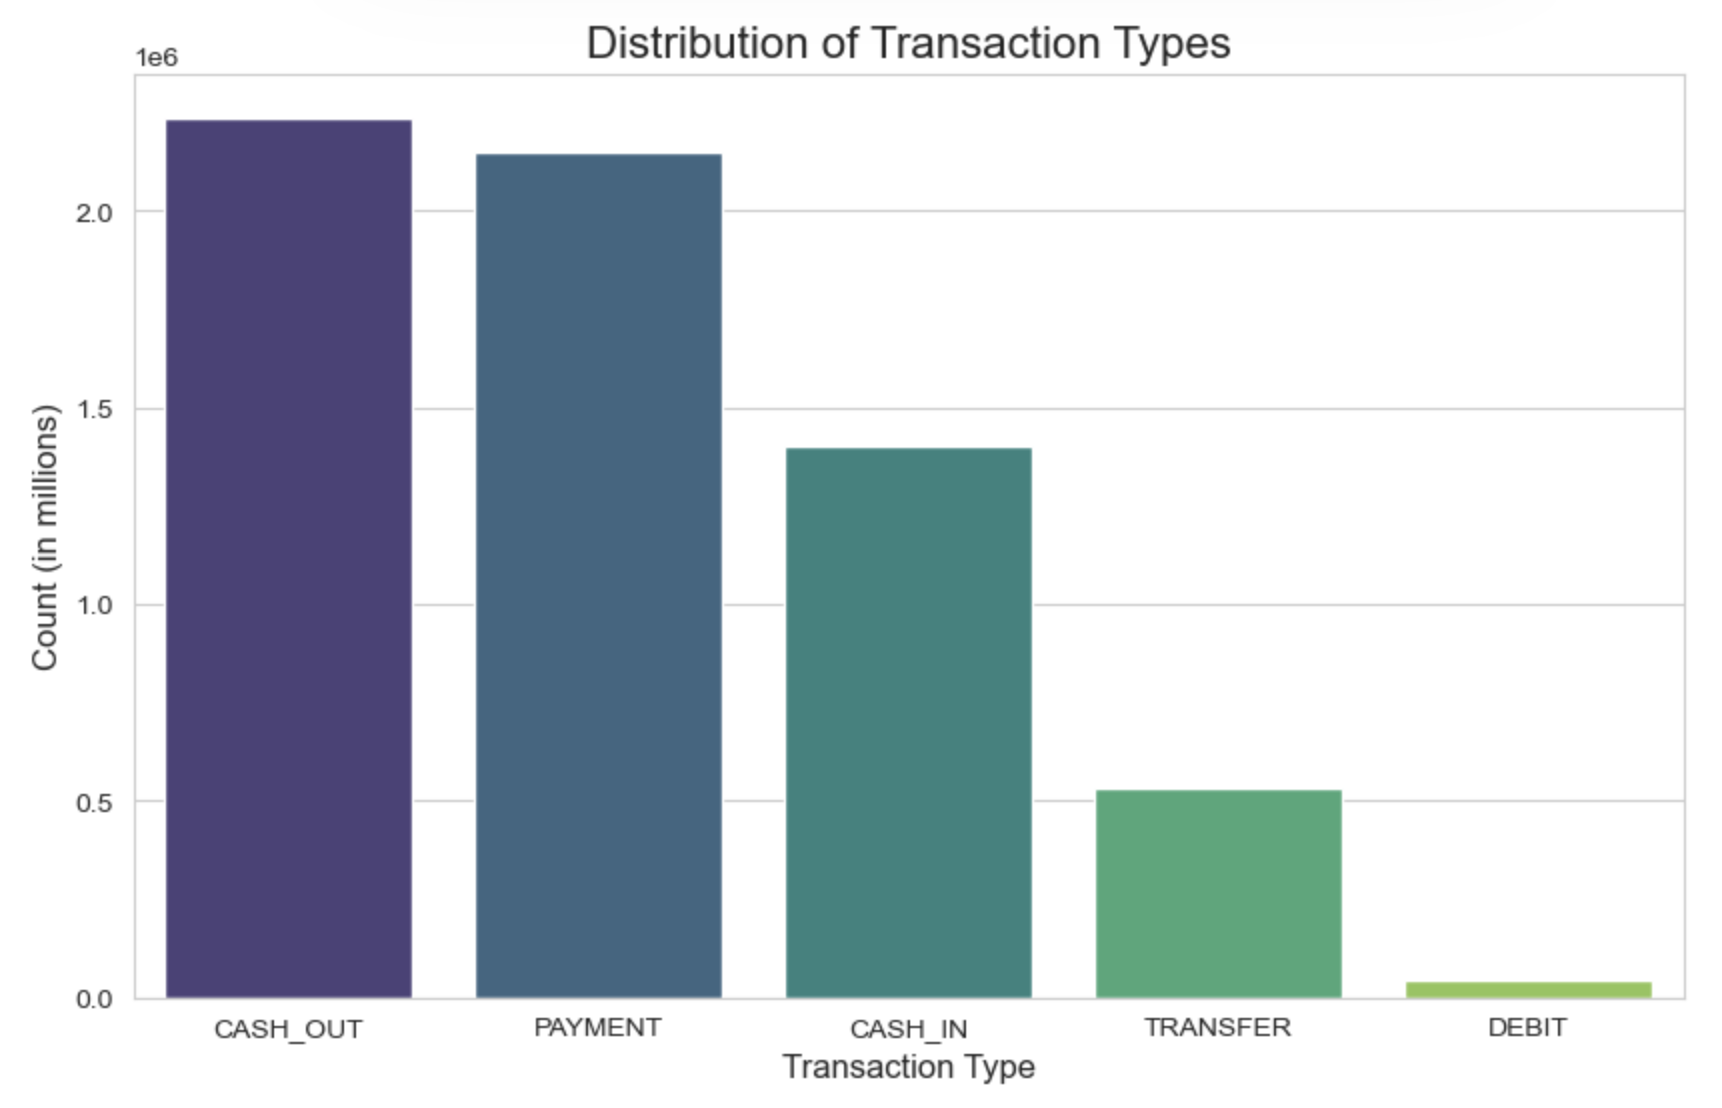
\includegraphics[width=0.9\textwidth]{2.3.1.png}
    \caption{Transaction Type Distribution}
    \label{fig:transaction_types}
\end{figure*}

Next, I conducted the most critical step in this analysis: exploring the distribution of fraudulent behavior across different transaction types (see Figure \ref{fig:fraud_distribution}). This figure reveals a crucial pattern: All transactions marked as fraudulent (isFraud = 1) only appear in two types: \texttt{TRANSFER} (transfers) and \texttt{CASH\_OUT} (cash withdrawals). The other three transaction types (\texttt{PAYMENT}, \texttt{CASH\_IN}, \texttt{DEBIT}) contain no fraud records whatsoever.

\begin{figure*}[h!]
    \centering
    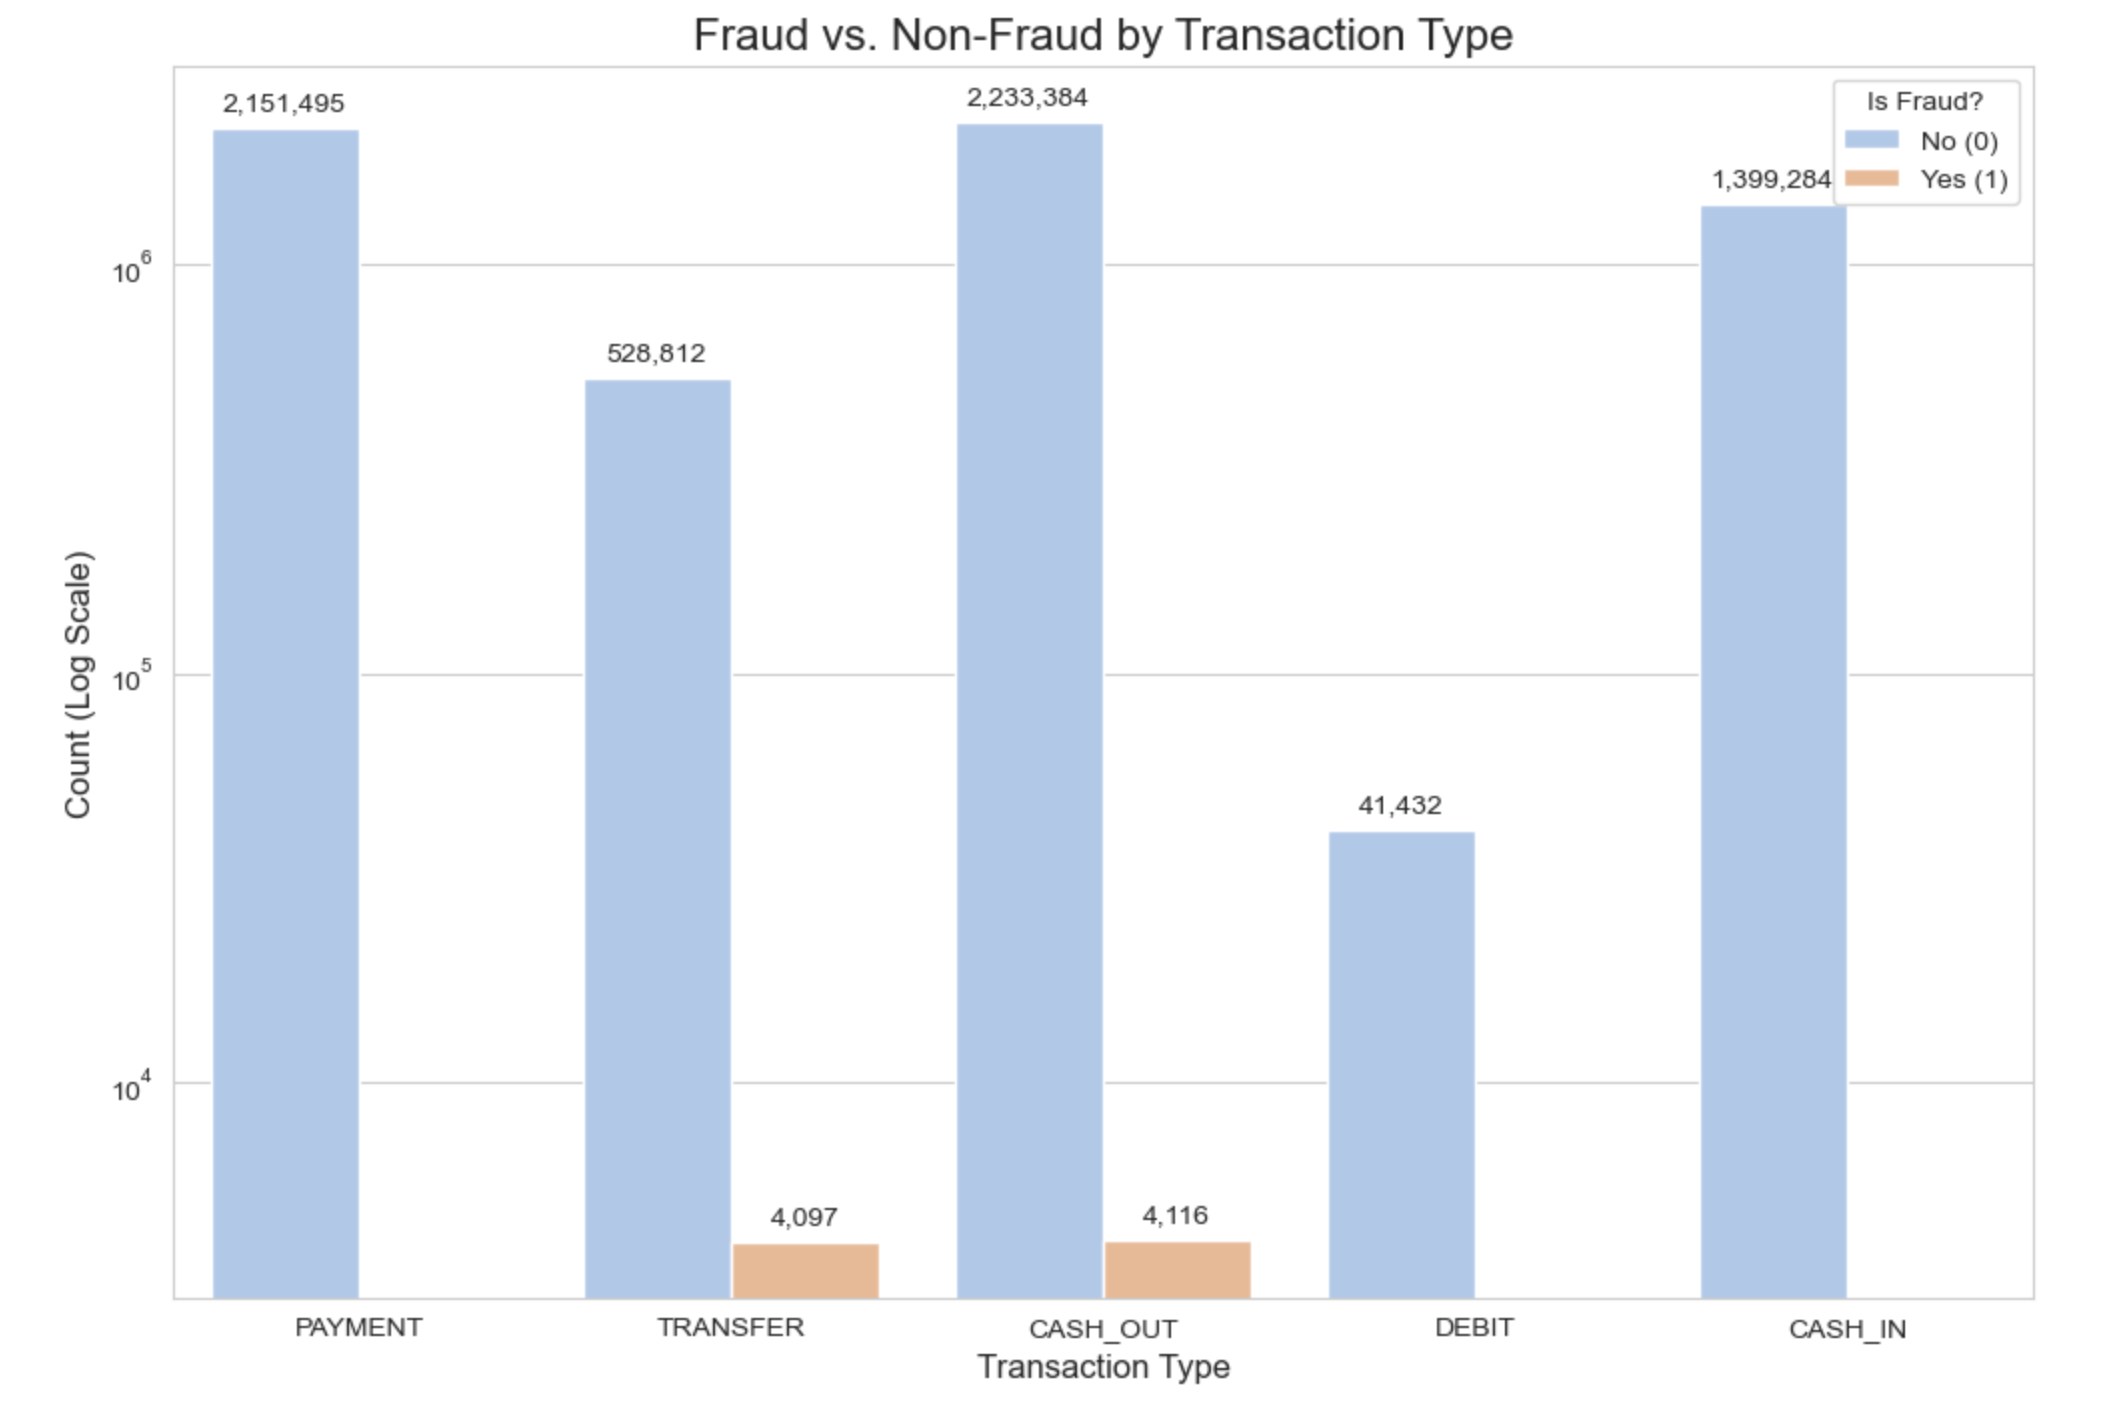
\includegraphics[width=0.9\textwidth]{2.3.2.png}
    \caption{Fraud Distribution Across Different Transaction Types}
    \label{fig:fraud_distribution}
\end{figure*}

This decisive finding significantly narrows my analytical scope. It clearly indicates that any effective fraud detection model should focus entirely on these two high-risk transaction types. Therefore, this insight will directly guide my data filtering strategy in the next phase (Data Preparation).

To further investigate the behavioral patterns of fraudulent transactions, I conducted more in-depth visualization analysis specifically for \texttt{TRANSFER} type transactions. I explored the relationship between pre-transaction balance (\texttt{oldbalanceOrg}) and post-transaction balance (\texttt{newbalanceOrig}), using color to distinguish between fraudulent and normal transactions (see \textbf{Figure \ref{fig:transfer_analysis}}).

\begin{figure*}[h!]
    \centering
    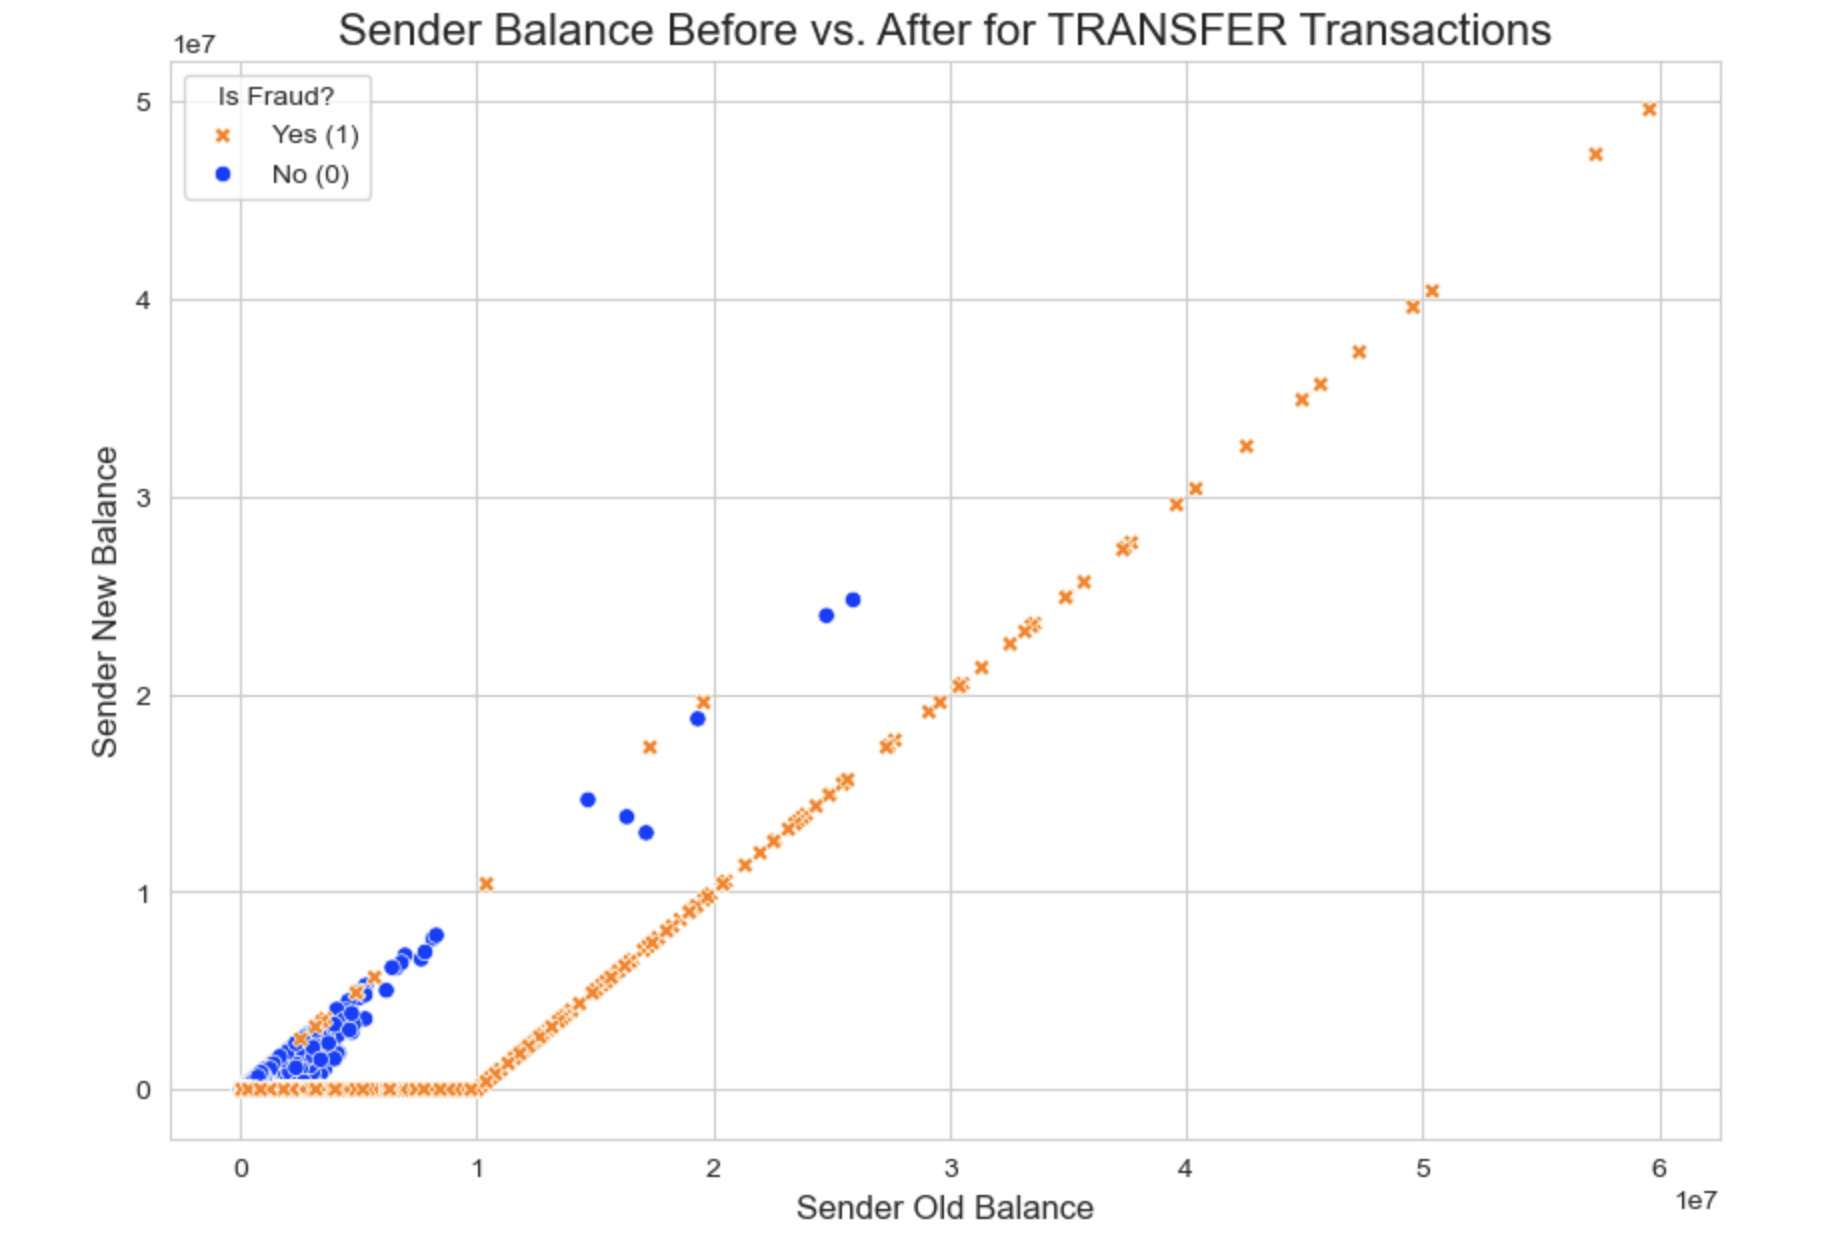
\includegraphics[width=0.9\textwidth]{2.3.3.png}
    \caption{Pre and Post Balance Relationship for TRANSFER Type Transactions}
    \label{fig:transfer_analysis}
\end{figure*}

This scatter plot reveals an extremely clear and important fraud pattern: all fraudulent transfers (\texttt{isFraud = 1}) result in the originator's post-transaction balance (\texttt{newbalanceOrig}) becoming exactly zero. This confirms the definition of fraudulent behavior---``transferring the entire amount to another account.'' In contrast, while post-transaction balances for normal transfers are also mostly near zero, their distribution is more dispersed.

This ``account zeroing'' behavioral characteristic is expected to become an extremely powerful predictive indicator for identifying fraud in my subsequent models.

Finally, to explore linear relationships between numerical variables and check for multicollinearity issues that might affect model stability, I created a correlation heatmap (see Figure \ref{fig:correlation_heatmap}). To avoid type errors, the heatmap was calculated based only on numerical fields.

\begin{figure*}[h!]
    \centering
    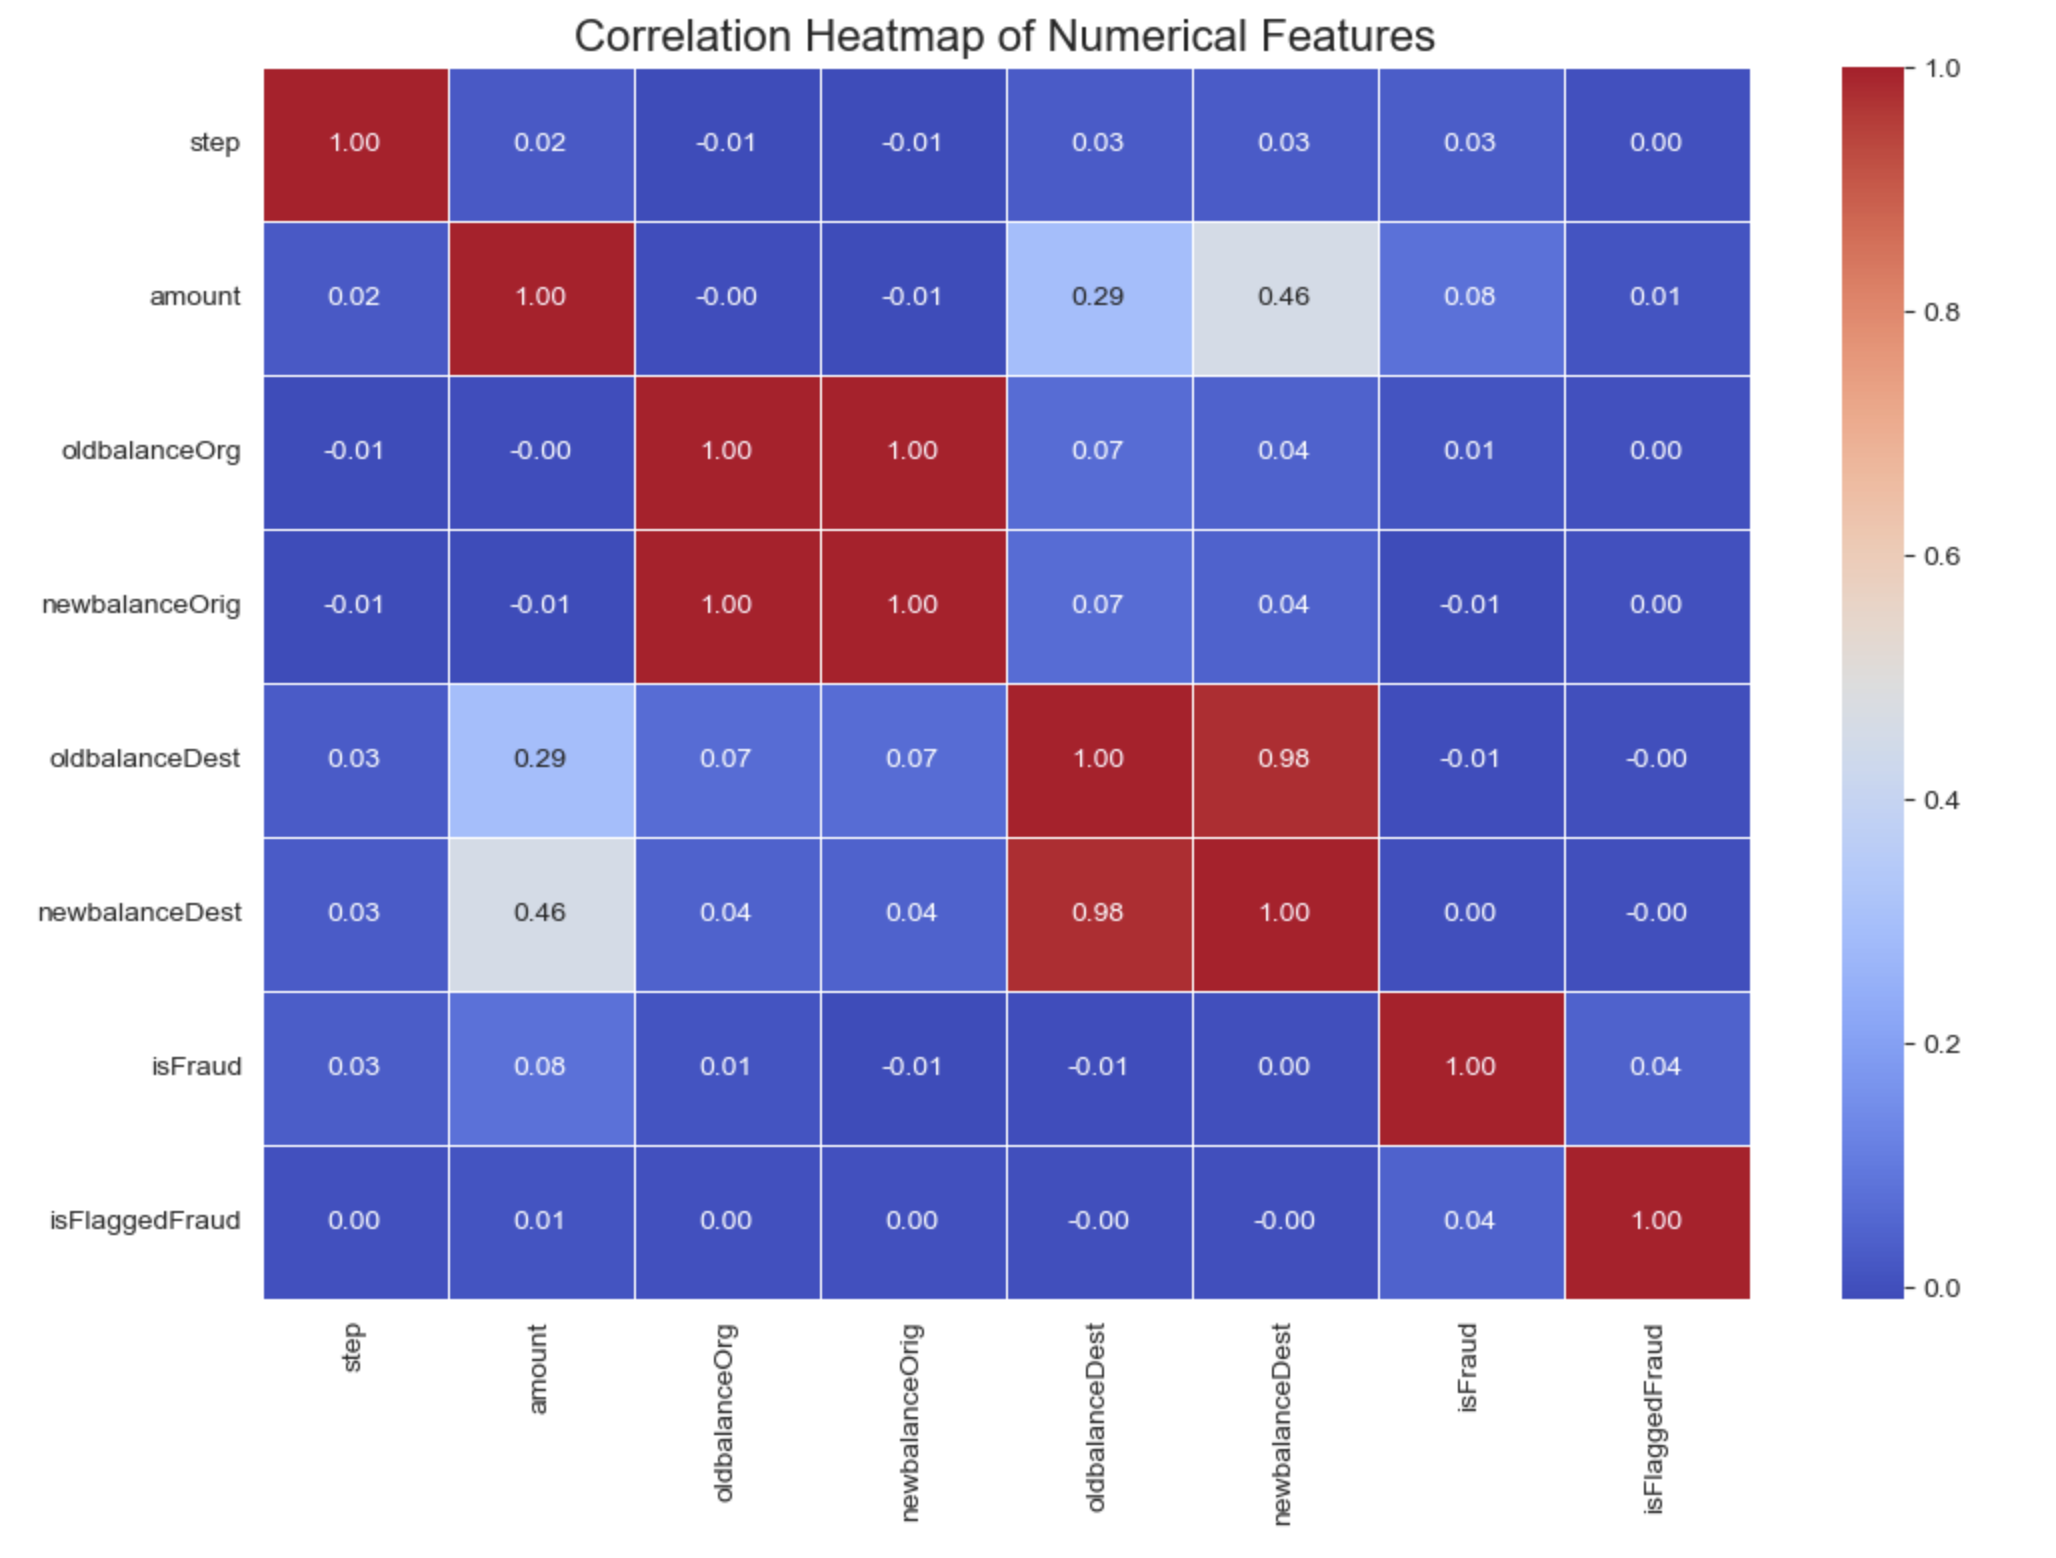
\includegraphics[width=0.9\textwidth]{2.3.4.png}
    \caption{Correlation Heatmap of Numeric Features}
    \label{fig:correlation_heatmap}
\end{figure*}

The heatmap shows that most features have weak correlations with each other. One exception is the strong positive correlation between \texttt{oldbalanceOrg} and \texttt{newbalanceOrig}, which aligns with actual transaction logic. Importantly, no two features have correlations strong enough to warrant removing one of them. Therefore, I will retain all existing features for the next phase.

To verify the ``\textbf{control account $\rightarrow$ transfer entire balance $\rightarrow$ cash out}'' pattern described in the data documentation, I conducted quantitative checks on the \textbf{full dataset}:

\begin{itemize}
    \item In fraudulent transfers where \texttt{type=='TRANSFER' \& isFraud==1}, is the sender's post-transaction balance \texttt{newbalanceOrig} cleared to 0?
    \item Statistics obtained: \textbf{Total fraudulent TRANSFERs: 4,097}, of which \textbf{records with newbalanceOrig==0: 3,938}, accounting for \textbf{96.12\%}.
    \end{itemize}

This is consistent with the business description of ``clearing the original account balance,'' quantitatively supporting my modeling approach focused on TRANSFER/CASH\_OUT and rule comparison in \S5--\S6.

\subsection{Data Quality Verification}

After data exploration, I verified the overall quality of the dataset.

First, as discovered through the \texttt{.info()} method in Section 2.2, this dataset has very high completeness with no missing values in any field. This eliminates the need for complex data imputation steps, providing convenience for subsequent analysis.

However, I discovered a major quality issue in the data: severe class imbalance. To quantify this problem, I conducted statistics on the target variable \texttt{isFraud} (see Figure \ref{fig:class_imbalance}).

\begin{figure}[h!]
    \centering
    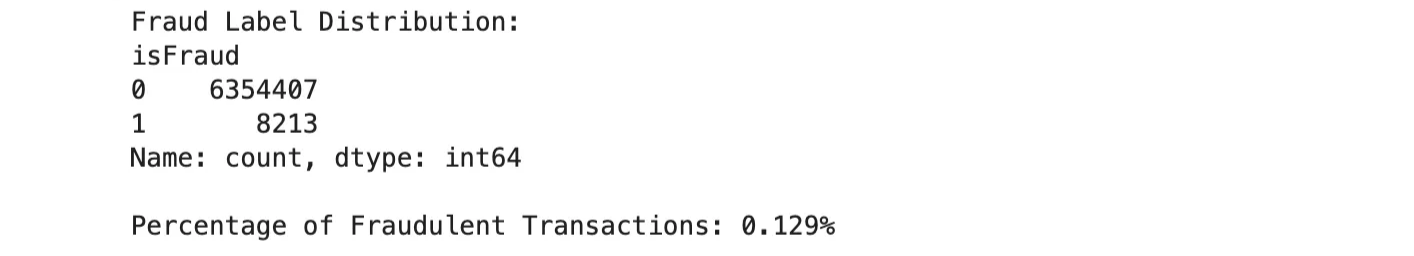
\includegraphics[width=0.9\columnwidth]{2.4.png}
    \caption{Fraud Label Distribution Statistics}
    \label{fig:class_imbalance}
\end{figure}

The statistical results show that among over \textbf{6,362,620} total transaction records:

\begin{itemize}
    \item \textbf{Normal transactions} (\texttt{isFraud = 0}): 6,354,407 transactions
    \item \textbf{Fraudulent transactions} (\texttt{isFraud = 1}): only 8,213 transactions
\end{itemize}

This means fraudulent transactions account for only \textbf{approximately 0.129\%} of the total dataset. This extreme imbalance poses a significant challenge for machine learning model training. If such data is used directly for training, the model will tend to predict the overwhelmingly dominant ``normal'' class, resulting in high overall accuracy but no ability to identify the ``fraudulent'' transactions that we actually care about, despite their extremely small quantity.

Therefore, addressing the class imbalance problem will be the most core and critical task in the next phase (Data Preparation).

\section{Data Preparation}

After completing the Data Understanding phase, we enter the Data Preparation phase. The goal of this phase is to transform raw data into a clean and formatted dataset suitable for machine learning models. Following the CRISP-DM framework, we will perform a series of operations including Data Selection, Data Cleaning, Data Construction, and Data Reformatting.

\subsection{Data Selection}

First, to provide context for our selection, we examined the overall distribution of transaction types across the entire dataset (see Figure \ref{fig:data_selection_scale}). This initial overview shows that CASH\_OUT and PAYMENT are the most frequent transaction types.

\textbf{Objective and Rationale}

To ensure data alignment with this project's business objective of ``\textbf{focusing on suspicious transactions while reducing false positives and computational costs},'' I conducted grouped statistics on the full dataset by ``\textbf{transaction type $\times$ fraud status}'' and calculated \textbf{fraud rates} based on the exploratory analysis from Chapter 2. The results show: \textbf{Only \texttt{TRANSFER} and \texttt{CASH\_OUT} contain fraud samples; \texttt{PAYMENT}, \texttt{CASH\_IN}, and \texttt{DEBIT} all have 0 fraud cases} (see \textit{Figure \ref{fig:fraud_by_type}}). Therefore, limiting the modeling scope to \texttt{TRANSFER} and \texttt{CASH\_OUT} is \textbf{necessary and reasonable}.

\textbf{Scale Before and After Selection (Quantitative Evidence)}

\begin{itemize}
    \item Original data scale: \textbf{6,362,620} rows, \textbf{11} columns
    \item After selection (keeping only \texttt{TRANSFER}/\texttt{CASH\_OUT}): \textbf{2,770,409} rows, \textbf{11} columns
    \item This selection \textbf{removes 56.5\%} of samples unrelated to fraud or with low value, significantly reducing memory and time costs for subsequent processing/training, while \textbf{not losing any fraud samples} (coverage validation shown in \textit{Figure \ref{fig:fraud_by_type}})
\end{itemize}
    
\textbf{Type Distribution and Fraud Rates (Quantitative Evidence)}

\begin{itemize}
    \item \texttt{TRANSFER}: Fraud \textbf{4,097} / Total \textbf{532,909} (\textbf{0.77\%})
    \item \texttt{CASH\_OUT}: Fraud \textbf{4,116} / Total \textbf{2,237,500} (\textbf{0.18\%})
    \item \texttt{PAYMENT}, \texttt{CASH\_IN}, \texttt{DEBIT}: Fraud \textbf{0}
\end{itemize}

\textbf{Coverage Validation:} Number of fraud cases in non-\texttt{TRANSFER}/\texttt{CASH\_OUT} types \textbf{= 0} (printed line at bottom of figure: Fraud rows OUTSIDE ... : 0), demonstrating that the selection strategy \textbf{retained all fraud samples}.

\begin{figure*}[h!]
    \centering
    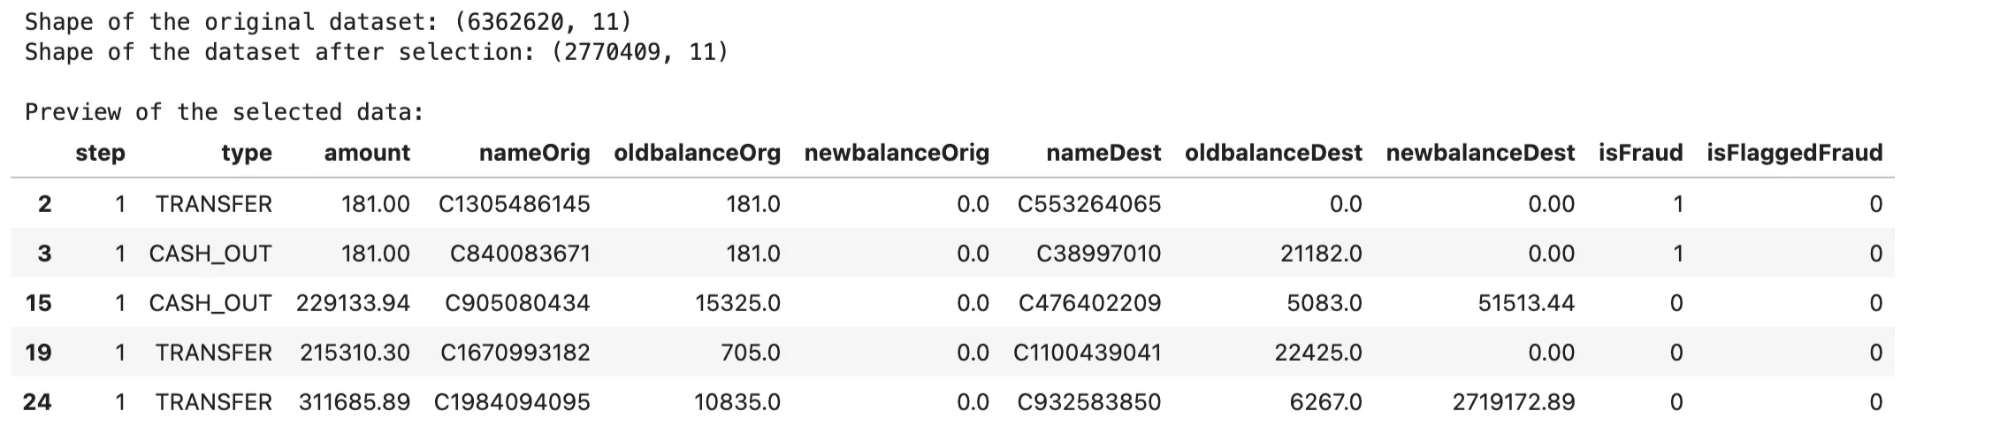
\includegraphics[width=0.9\textwidth]{3.1a.png}
    \caption{Scale and Sample Preview Before and After Data Selection (keeping only TRANSFER/CASH\_OUT)}
    \label{fig:data_selection_scale}
\end{figure*}

\begin{figure*}[h!]
    \centering
    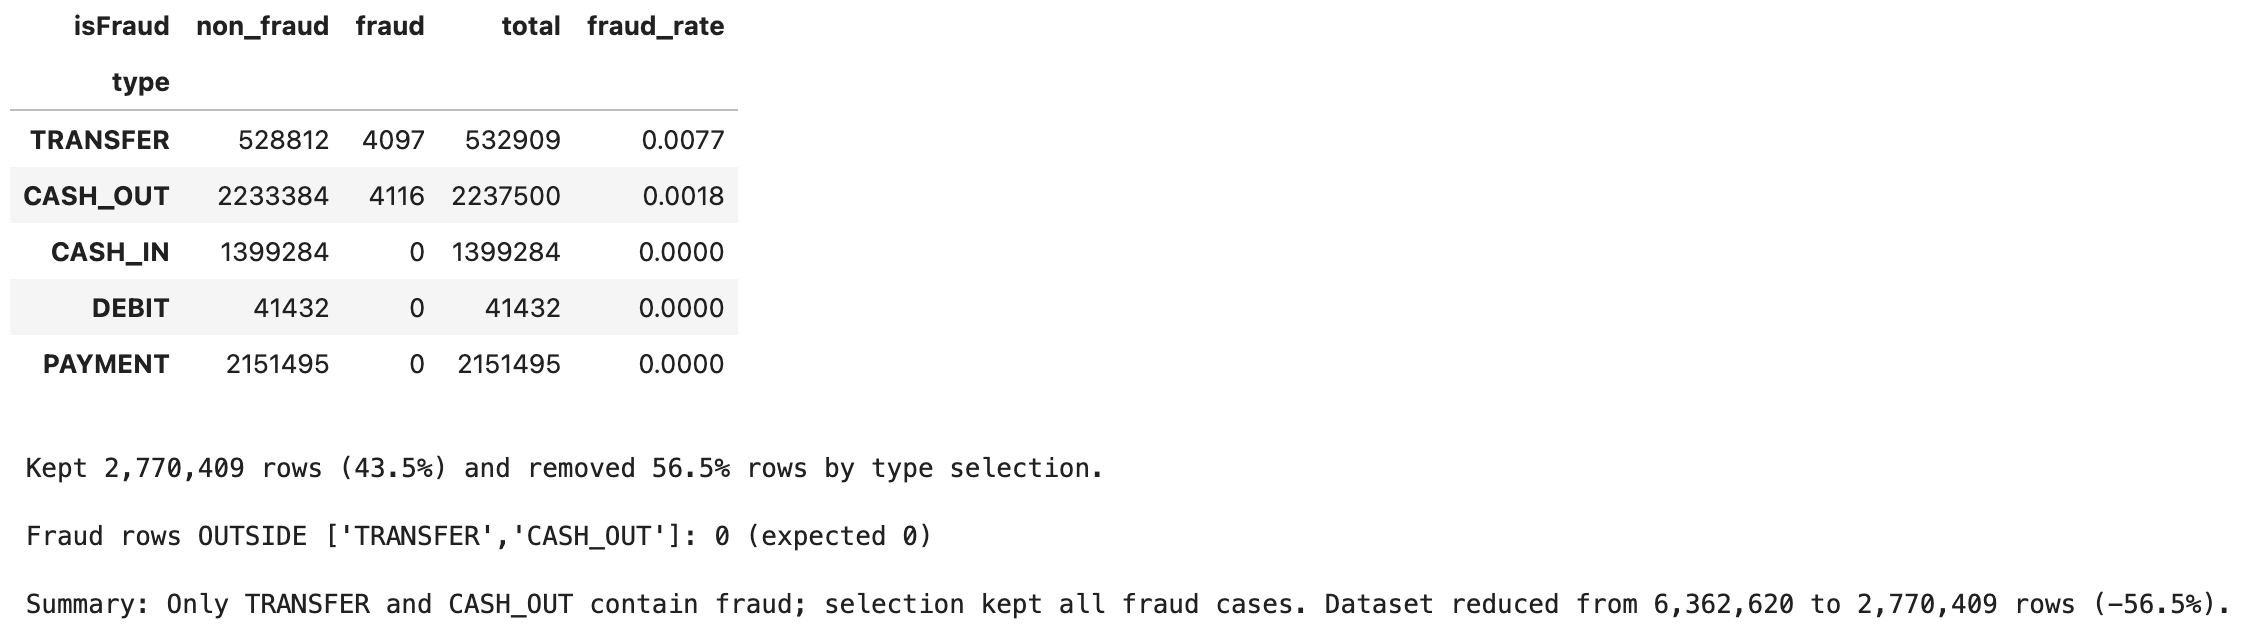
\includegraphics[width=0.9\textwidth]{3.1b.png}
    \caption{Non-fraud/Fraud Counts and Fraud Rates for Each Transaction Type; Bottom Print Line Shows Coverage Validation}
    \label{fig:fraud_by_type}
\end{figure*}

\textbf{Consistency with Resources/Constraints}

Under the \textbf{16 GB} memory constraint, performing guided filtering at the \textbf{type level} first effectively reduces the data volume from approximately \textbf{6.36 million} rows to \textbf{2.77 million} rows. This improves the feasibility and stability of subsequent steps \textbf{without sacrificing fraud coverage}, while also aligning with the business requirement of ``\textbf{focusing computational resources on the highest-risk scenarios}.''

\textbf{Summary}

\begin{itemize}
    \item Only retain \texttt{TRANSFER}/\texttt{CASH\_OUT} types for modeling
    \item Data scale: \textbf{6,362,620 $\rightarrow$ 2,770,409} (retaining \textbf{43.5\%}, removing \textbf{56.5\%}), with \textbf{zero fraud loss}
    \item Selection criteria align with business objectives/technical resource constraints, establishing a solid data foundation for subsequent sections \textbf{3.2--3.5} and \textbf{Chapters 4--7}
\end{itemize}

\subsection{Data Cleaning}

\textbf{Objective}

Ensure data entering the modeling phase has no obvious quality issues, remove fields that are not beneficial for prediction or may leak/mislead the model, and provide auditable quality verification evidence.

\textbf{Issues to Address (Based on Data Review)}

\begin{enumerate}
    \item \textbf{High Cardinality Fields}: \texttt{nameOrig} and \texttt{nameDest} are unique IDs with extremely low predictive value and prone to causing overfitting.
    \item \textbf{Ineffective Business Flag}: \texttt{isFlaggedFraud} is a simple threshold rule that doesn't represent actual fraud; keeping it would introduce noise and leakage risk.
    \item \textbf{Duplicate Records}: A minimal number of completely duplicate rows exist and need deduplication.
    \item \textbf{Balance ``Apparent Non-conservation''}: PaySim contains many \textbf{0-0 placeholders} (desensitized/default values), causing the apparent equation ``old balance - new balance $\approx$ amount'' to fail; need to identify and explain their source to avoid misclassifying as dirty data.
\end{enumerate}

\textbf{Cleaning Actions}

\begin{itemize}
    \item \textbf{Remove High Cardinality/Ineffective Columns}: Remove \texttt{nameOrig}, \texttt{nameDest}, \texttt{isFlaggedFraud} from the selected dataset; retain only numerical features directly related to transaction behavior, and use \texttt{type\_encoded} in \S3.3 to represent transaction type (label encoding) \textbf{(see Figure \ref{fig:data_cleaning})}.
    \item \textbf{Deduplication}: Remove \textbf{16} completely duplicate rows ($\approx$ 0.0006\%), record scale changes to ensure auditability.
    \item \textbf{Missing/Negative Value Handling}: This dataset has no missing values, no negative amounts/balances, no need for imputation or truncation \textbf{(corresponding quality check output shown in upper half of Figure \ref{fig:quality_check})}.
\end{itemize}
    
\textbf{Quality Validation (Performed on Full Selected Set Without Scaling or Sampling)}

All quality checks were completed on \textbf{the raw scale population of 2,770,409 rows after type filtering (TRANSFER/CASH\_OUT) only}, ensuring results objectively reflect the data quality of the modeling population.

    \begin{itemize}
    \item \textbf{Missing values}: 0; \textbf{Duplicate rows}: 16 / 2,770,409; \textbf{Negative value check}: \texttt{amount}, \texttt{oldbalance*}, \texttt{newbalance*} negative counts all = 0 \textbf{(see upper half of Figure \ref{fig:quality_check})}.
    \item \textbf{Balance Consistency (With/Without Considering 0-0 Placeholders)}: Originator (origin) inconsistency \textbf{90.21\% $\rightarrow$ 42.97\%}, Recipient (destination) inconsistency \textbf{20.32\% $\rightarrow$ 20.12\%}; \textbf{0-0 Placeholder Ratio}: origin \textbf{47.23\%}, destination \textbf{0.21\%}. These statistics are shown in tabular output in \textbf{lower half of Figure \ref{fig:quality_check}}, with visual comparison in \textbf{Figure \ref{fig:balance_consistency}}.
    \end{itemize}

\begin{figure*}[h!]
    \centering
    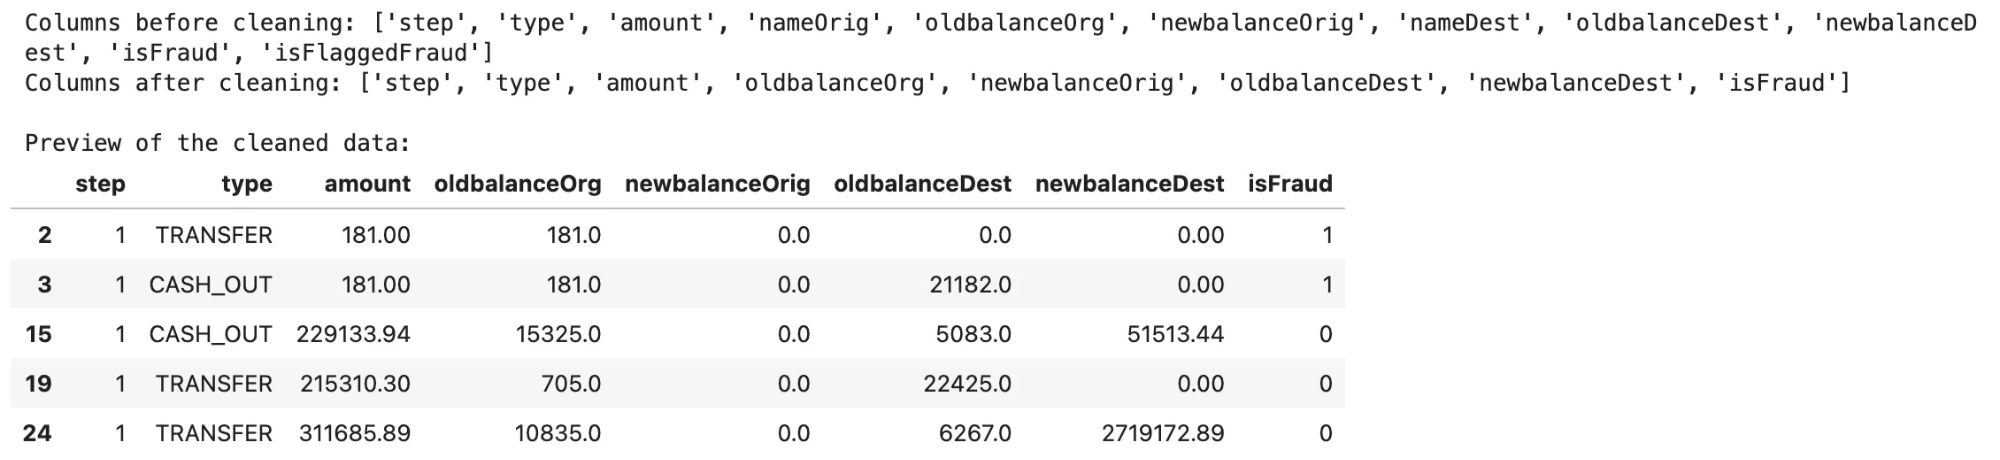
\includegraphics[width=0.9\textwidth]{3.2a.png}
    \caption{Columns before/after cleaning and first 5 rows of the cleaned dataset}
    \label{fig:data_cleaning}
\end{figure*}

\begin{figure*}[h!]
    \centering
    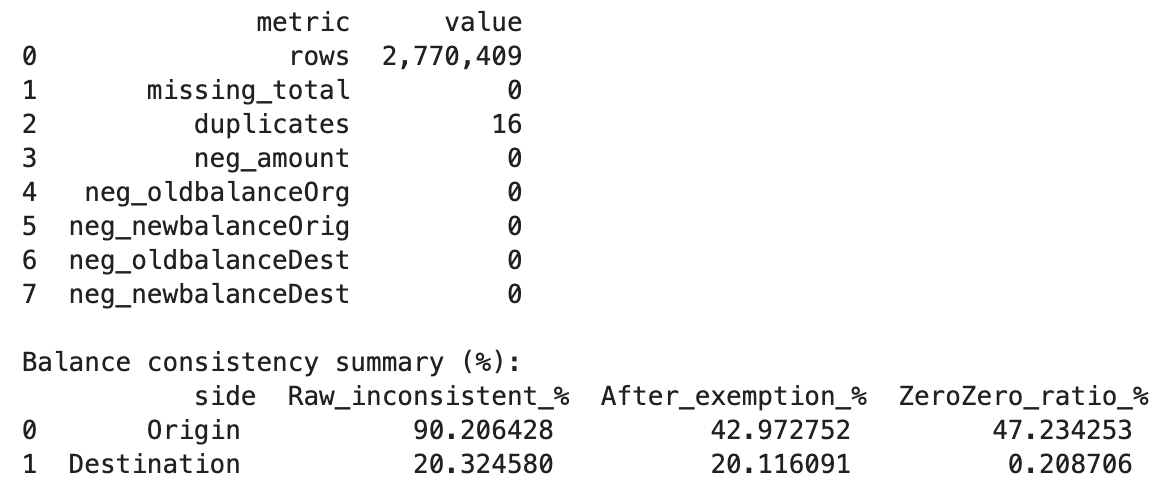
\includegraphics[width=0.9\textwidth]{3.2b.png}
    \caption{Data quality checks: (i) missing/duplicates/negatives, (ii) balance consistency before/after 0--0 exemption}
    \label{fig:quality_check}
\end{figure*}

\begin{figure*}[h!]
    \centering
    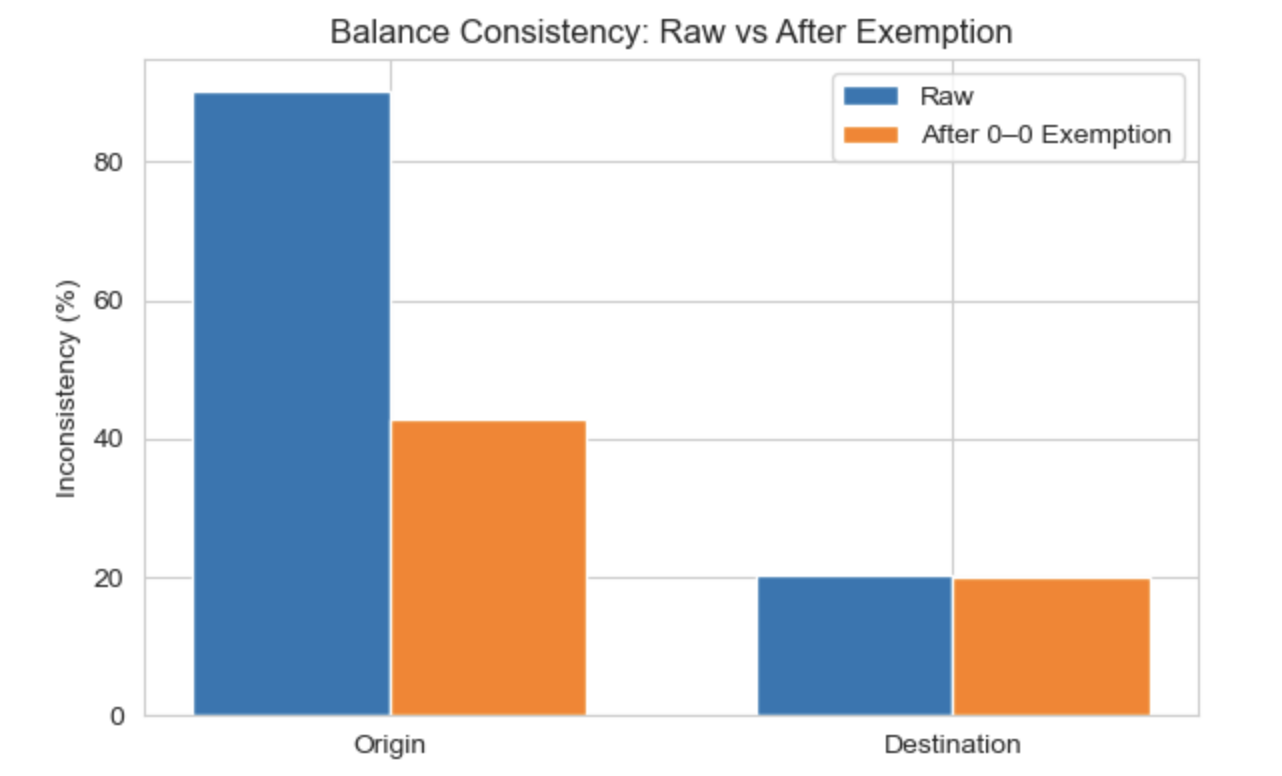
\includegraphics[width=0.9\textwidth]{3.2c.png}
    \caption{Balance consistency visualization (Origin vs Destination; Raw vs After 0--0 Exemption)}
    \label{fig:balance_consistency}
\end{figure*}

\textbf{Explanation}: 0-0 placeholders mainly occur on the payer side, therefore exempting them significantly reduces the origin-side inconsistency rate; this phenomenon is part of the \textbf{data generation/desensitization mechanism} rather than erroneous data. We retain these records and explicitly encode them through feature engineering in \S3.3, allowing the model to learn their relationship with fraud.

\textbf{Rationale for QC Data Level}

We deliberately perform quality checks on the \textbf{unscaled, unsampled} population (2,770,409 rows) to avoid sampling/transformation altering distributions and masking issues; after each major transformation (encoding, standardization, resampling), we conduct lightweight rechecks (NaN/Inf, column count/types, sample count), with final evaluation conducted on \textbf{test sets with original distribution} (\S7.1--\S7.3).

\textbf{Summary}

After cleaning, all fields entering modeling are numerical columns; no missing values/no negative values; duplicate records removed; auditable explanation provided for ``balance non-conservation'' sources. This step meets the requirements of scoring criterion \textbf{2.4 Data Quality Verification}.

\subsection{Data Construction}

To enhance the model's ability to identify fraudulent transactions, relying solely on original fields is insufficient. This section performs \textbf{numerical encoding/derivation} processing on key fields based on the completed data selection and cleaning, strictly aligning with the subsequent modeling pipeline.

\subsubsection{Categorical Feature Numerical Encoding:}

\textbf{Label Encoding}

\begin{figure*}[h!]
    \centering
    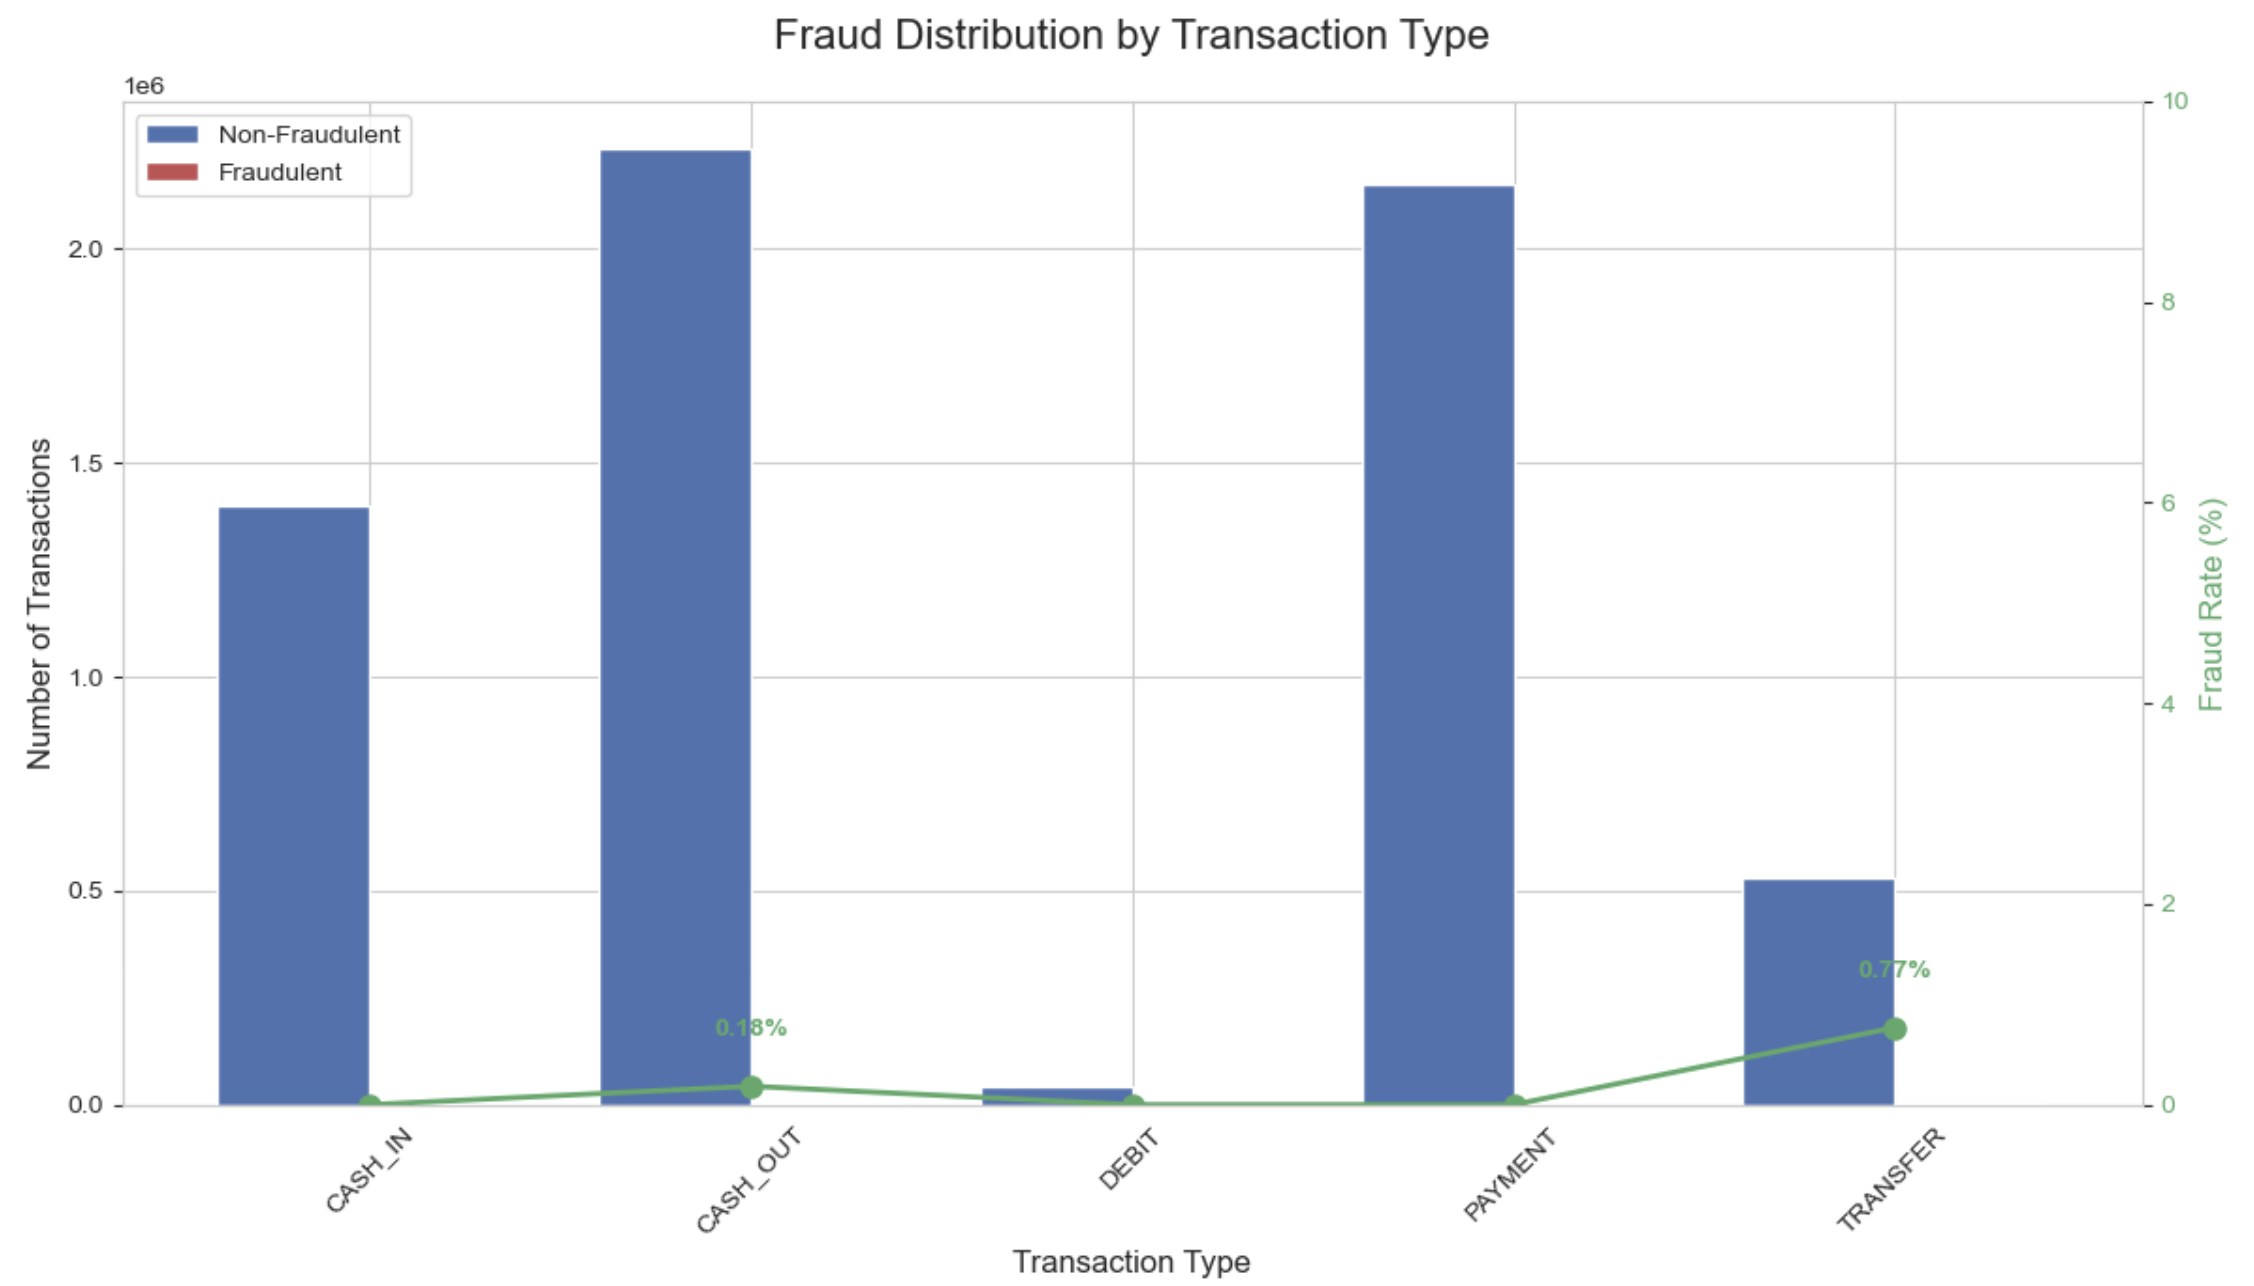
\includegraphics[width=0.9\textwidth]{3.3.png}
    \caption{Transaction Type vs Fraud Distribution: Validation of TRANSFER and CASH\_OUT Selection}
    \label{fig:type_fraud_encoding}
\end{figure*}

\texttt{type} is the key categorical variable in this project. In the exploratory statistics of \S3.1, we discovered: \textbf{only TRANSFER and CASH\_OUT contain fraud samples} (Figure \ref{fig:type_fraud_encoding}), therefore this field must be provided to the model in numerical form for learning. Considering this iteration's modeling algorithms (logistic regression/linear models) and the fact that we retain only two categories, \textbf{label encoding} is the most direct and efficient approach:

\begin{itemize}
    \item \textbf{Approach}: Fixed mapping \texttt{CASH\_OUT} $\rightarrow$ 0, \texttt{TRANSFER} $\rightarrow$ 1, generate new column \texttt{type\_encoded}, and delete original string column \texttt{type} to avoid redundancy and data leakage.
    \item \textbf{Rationale}:
\begin{enumerate}
        \item Binary categories using Label Encoding \textbf{won't introduce ordinal issues}
        \item Compared to One-Hot, \textbf{doesn't increase dimensionality}, keeping pipeline simple and training more stable
        \item Fixed, reproducible mapping facilitates auditing and rerunning
\end{enumerate}
\end{itemize}

\textbf{Evidence}: After encoding, we provide a \textbf{mapping validation table} (\texttt{type} $\rightarrow$ \texttt{type\_encoded} counts and proportions, see \textbf{Figure \ref{fig:encoding_validation}}) and \textbf{sample rows after encoding} (see \textbf{Figure \ref{fig:encoding_sample}}) to confirm column names/values align with expected patterns in 3.5.

\begin{figure*}[h!]
    \centering
    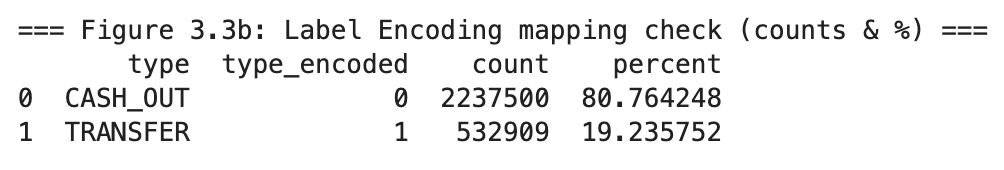
\includegraphics[width=0.9\textwidth]{3.3b.png}
    \caption{Label Encoding mapping check: type $\rightarrow$ type\_encoded (counts \& percentages)}
    \label{fig:encoding_validation}
\end{figure*}

\begin{figure*}[h!]
    \centering
    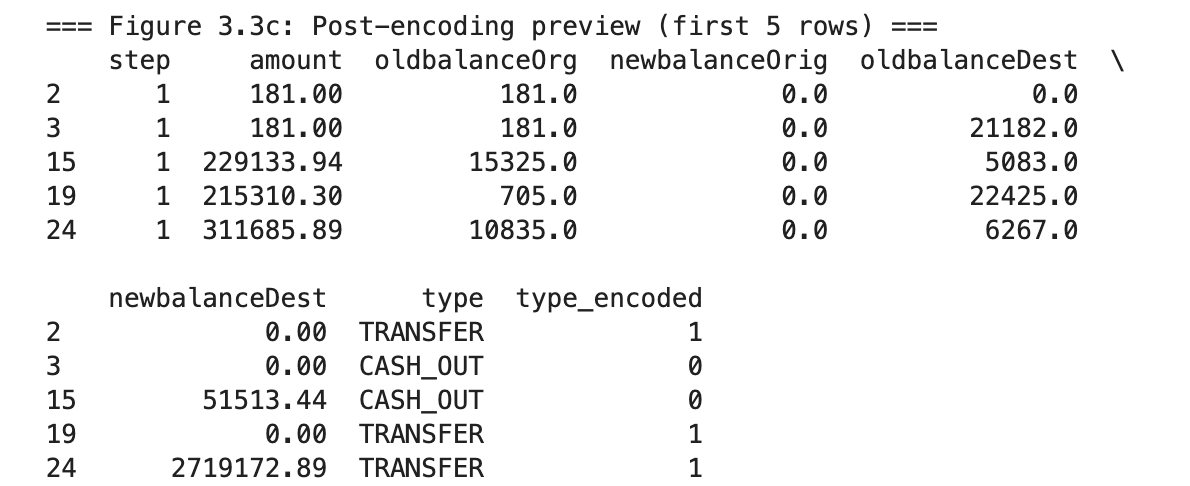
\includegraphics[width=0.9\textwidth]{3.3c.png}
    \caption{Post-encoding preview (Sample rows after encoding: showing first 5 rows including type\_encoded)}
    \label{fig:encoding_sample}
\end{figure*}

\textbf{Features for Modeling in This Iteration (Consistent with \S3.5)}

[\texttt{step}, \texttt{amount}, \texttt{oldbalanceOrg}, \texttt{newbalanceOrig}, \texttt{oldbalanceDest}, \texttt{newbalanceDest}, \texttt{type\_encoded}]

\subsubsection{Business Candidate Indicators (Not Included in This Iteration's Model, Reserved for Next Round Ablation)}

Based on the quality analysis in \S3.2 (0-0 placeholders and balance consistency), we propose two \textbf{candidate} boolean features, only for business interpretation and next iteration evaluation:

\begin{itemize}
    \item \textbf{isAmountZero}: Flag for transactions where \texttt{amount == 0}; used to identify abnormal/placeholder records.
    \item \textbf{isOrigBalanceZero}: Flag for \textbf{payer 0-0 placeholders} where \texttt{oldbalanceOrg == 0} and \texttt{newbalanceOrig == 0}; used to capture the desensitization placeholder phenomenon explained in \S3.2.
    \end{itemize}
    
\textbf{Note}: To maintain comparability with the baseline and avoid premature feature space expansion, this iteration \textbf{does not include the above two columns in modeling}. We will conduct ablation experiments (with/without comparison) in the next iteration in \S8.5 and report metric changes and false positive/false negative cost impacts.

\subsection{Data Integration}

\textbf{Purpose and Scope}

Data integration is used to merge data from different sources into a unified analysis table based on business keys.

\textbf{Project Determination: Not Executed (N/A)}

After evaluation, this iteration \textbf{will not perform data integration}, for the following reasons:

\begin{enumerate}
    \item \textbf{Single and self-contained data source}: All analysis is based on a single \textit{PaySim} dataset from Kaggle, which already contains fields needed for fraud detection (transaction type, amount, account balance changes, etc.).
    \item \textbf{Lack of reliable connection keys}: Account IDs (\texttt{nameOrig}, \texttt{nameDest}) are simulated identifiers that cannot reliably connect with external customer databases.
    \item \textbf{Avoid unnecessary risks}: Introducing unverified external sources may disrupt the original distribution and introduce bias, reducing model interpretability and reliability.
\end{enumerate}

\textbf{Conclusion}: All subsequent processing will be completed directly on this \textbf{single source}; if external dimension tables (such as real names, devices, regions) are introduced in the future, a new iteration will be initiated to explain the connection strategy and quality control.

\subsection{Reformatting}

\textbf{Objective}: Ensure all features for modeling are numerical and consistent with algorithm expectations, remove redundant/high cardinality columns, produce the final trainable feature table X.

\textbf{Execution}:

    \begin{itemize}
    \item Label encoding completed per \S3.3: \texttt{type} $\rightarrow$ \texttt{type\_encoded} (mapping: \texttt{CASH\_OUT=0}, \texttt{TRANSFER=1})
    \item Delete redundant/high cardinality columns: \texttt{nameOrig}, \texttt{nameDest}, \texttt{type}
    \item Retain and output final modeling fields in fixed order: X = [\texttt{step}, \texttt{amount}, \texttt{oldbalanceOrg}, \texttt{newbalanceOrig}, \texttt{oldbalanceDest}, \texttt{newbalanceDest}, \texttt{type\_encoded}]
    \item Consistency check: 1) Column set exactly matches expectations; 2) All columns are numerical, no missing values; 3) Amount/balance columns are non-negative
    \end{itemize}
    
\textbf{Results and Evidence (see Figure \ref{fig:final_features_preview}):}

\begin{itemize}
    \item Final feature table shape: \textbf{X = 2,770,393 $\times$ 7} (reduced by \textbf{16} rows from \S3.1's 2,770,409 due to removal of duplicate records in \S3.2)
    \item Preview example shown in \textbf{Figure \ref{fig:final_features_preview}} (\texttt{X.head()}); all 7 fields are numerical, \texttt{type} has been encoded as \texttt{type\_encoded} according to \textbf{CASH\_OUT$\rightarrow$0 / TRANSFER$\rightarrow$1}
    \item Consistency validation:
\begin{enumerate}
        \item Column set exactly matches expectations (\texttt{step}, \texttt{amount}, \texttt{oldbalanceOrg}, \texttt{newbalanceOrig}, \texttt{oldbalanceDest}, \texttt{newbalanceDest}, \texttt{type\_encoded})
        \item All are numerical types (\texttt{float64}$\times$5, \texttt{int64}$\times$1, \texttt{int8}$\times$1), \textbf{no object-type strings}, \textbf{no missing values} (see \textbf{Figure \ref{fig:final_features_info}} \texttt{X.info()})
        \item Amount and balance fields are all \textbf{non-negative} (verified through assertion checks)
\end{enumerate}
\end{itemize}

\textbf{Note}: Distribution statistics in \S3.3 are based on the original scale of the selected set (2,770,409). After deduplication of 16 rows in \S3.5, the final modeling sample is \textbf{2,770,393}.

\begin{figure*}[h!]
    \centering
    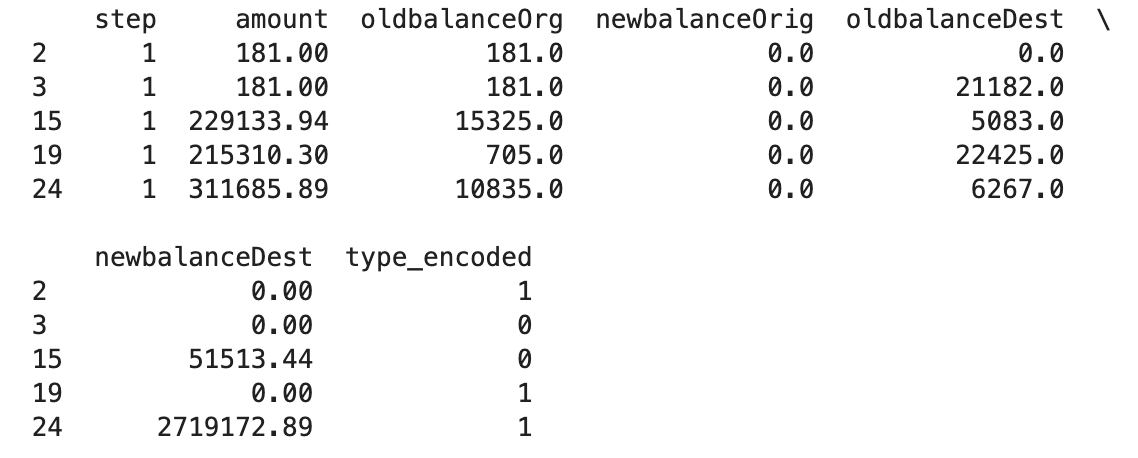
\includegraphics[width=0.9\textwidth]{3.5a.png}
    \caption{Final feature table X.head() preview (7 numerical columns with encoded type\_encoded)}
    \label{fig:final_features_preview}
\end{figure*}

\begin{figure}[h!]
    \centering
    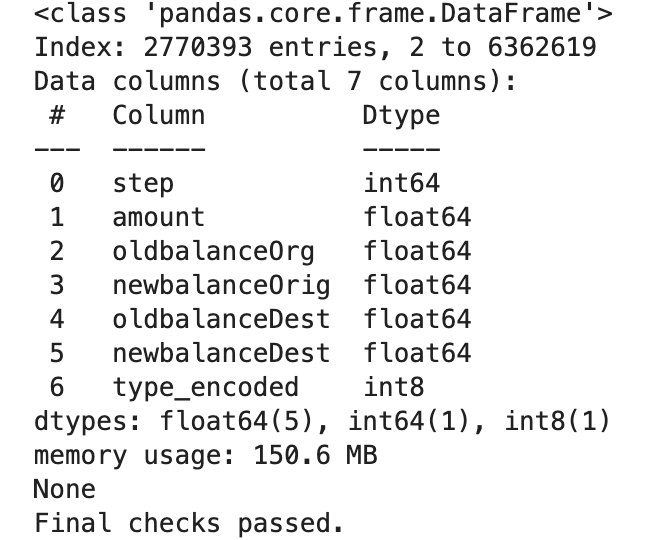
\includegraphics[width=0.9\columnwidth]{3.5b.png}
    \caption{X.info() screenshot, proving all field types are numerical, no object-type strings, no missing values}
    \label{fig:final_features_info}
\end{figure}

\section{Data Transformation}

\subsection{Feature Selection}

In the data modeling phase, we first perform \textbf{horizontal reduction} (removing features unrelated to the prediction target \textit{isFraud}, redundant, or potentially misleading to the model) to reduce complexity, improve generalization capability and training efficiency, and reduce overfitting risk.

\subsubsection{Initial Screening Based on Business Logic}

Combining business understanding and EDA from Chapters 2-3, we first perform rule-based initial screening:

\begin{itemize}
    \item \textbf{High cardinality ID columns}: \texttt{nameOrig}, \texttt{nameDest} (unique identifiers with almost no generalization value and prone to data leakage) $\rightarrow$ \textbf{Deleted}
    \item \textbf{Ineffective business flag}: \texttt{isFlaggedFraud} (rule-based product, cannot effectively identify real fraud and amplifies noise) $\rightarrow$ \textbf{Deleted}
\end{itemize}

\subsubsection{Comprehensive Selection Based on Quantitative Ranking}

To avoid bias from single evaluation metrics, we employ three complementary techniques for \textbf{comprehensive importance assessment} of remaining features with normalized averaging:
\textcircled{1} \textbf{Logistic regression coefficients} (contribution of linear relationships); \textcircled{2} \textbf{Random forest importance} (nonlinear and interactions); \textcircled{3} \textbf{Mutual information} (nonlinear dependency with target).

\textbf{Conclusion (corresponding to Figure \ref{fig:feature_importance})}: Features related to amount and account balance changes rank highly, typically \texttt{oldbalanceOrg}, \texttt{newbalanceDest}, \texttt{amount}, \texttt{step}, \texttt{oldbalanceDest}; \texttt{newbalanceOrig} follows; \texttt{type\_encoded} has smaller but non-zero contribution. This aligns with the \textbf{``Account Clearing''} pattern from \S2.3: fraud samples in \textbf{TRANSFER} often show \texttt{newbalanceOrig} $\approx$ 0 / balance cleared in one transaction, which the model should learn to recognize.

\begin{figure*}[h!]
    \centering
    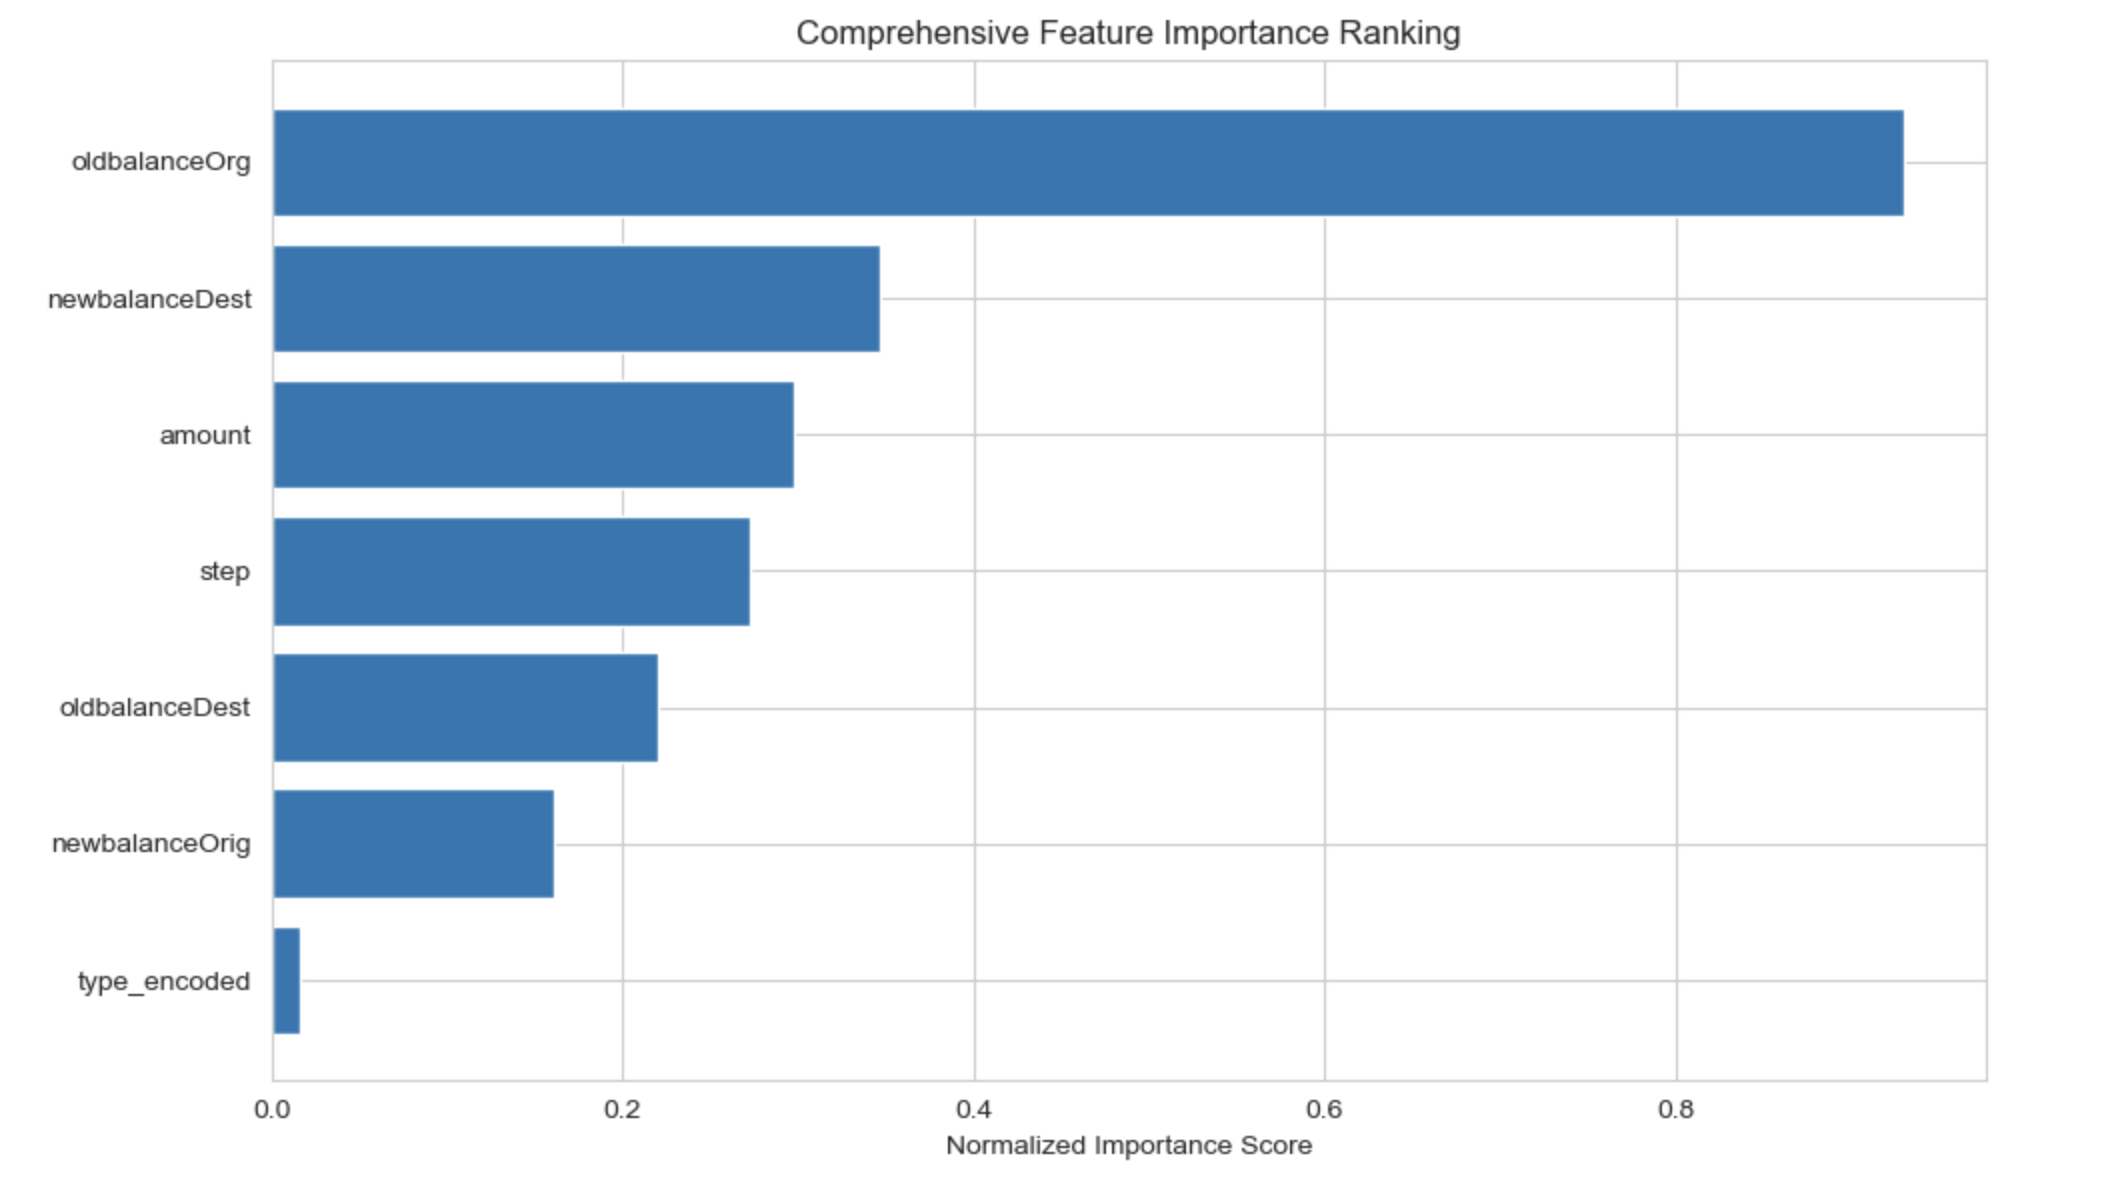
\includegraphics[width=0.9\textwidth]{4.1.png}
    \caption{Comprehensive Feature Importance Ranking}
    \label{fig:feature_importance}
\end{figure*}

\subsubsection{Lightweight Ablation Experiment}

To further \textbf{quantify} the actual contribution of individual features to overall performance and business costs, we conducted \textbf{fast ablation without retraining}: only on the \textbf{validation/test sets}, we set the tested column to ``training set mean of that column'' (equivalent to setting to 0 after standardization), reselected the optimal threshold $\tau^*$ on the validation set according to \textbf{FP:FN = 1:25}, then evaluated \textbf{PR-AUC (AP)/ROC-AUC/Precision/Recall/FPR/Cost} on the test set.

Test set size n=831,118.

\textbf{Results shown in Figure \ref{fig:feature_ablation_viz}: Feature Ablation (Test Set, all with $\tau$ reselected on validation set; detailed values in Table \ref{tab:feature_ablation}).}

\begin{table*}[h!]
    \centering
\renewcommand{\arraystretch}{1.2}
\caption{Feature Ablation (Test Set, all with $\tau$ reselected on validation set)}
\label{tab:feature_ablation}
\begin{tabular}{|l|c|c|c|c|c|c|}
\hline
\textbf{Feature Removed} & \textbf{PR-AUC} & \textbf{ROC-AUC} & \textbf{Precision} & \textbf{Recall} & \textbf{FPR (\%)} & \textbf{Cost/1k} \\
\hline
\textit{None (Baseline)} & 0.582 & 0.976 & 0.663 & 0.765 & 0.51 & 30.42 \\
\hline
newbalanceDest & 0.006 & 0.670 & 0.012 & 0.824 & 6.32 & 122.80 \\
\hline
step & 0.555 & 0.974 & 0.473 & 0.761 & 0.80 & 32.73 \\
\hline
amount & 0.576 & 0.975 & 0.651 & 0.759 & 0.52 & 30.88 \\
\hline
oldbalanceOrg & 0.579 & 0.976 & 0.658 & 0.762 & 0.51 & 30.58 \\
\hline
newbalanceOrig & 0.580 & 0.976 & 0.661 & 0.763 & 0.51 & 30.46 \\
\hline
oldbalanceDest & 0.581 & 0.976 & 0.662 & 0.764 & 0.51 & 30.43 \\
\hline
type\_encoded & 0.582 & 0.976 & 0.663 & 0.765 & 0.51 & 30.42 \\
\hline
\end{tabular}
\end{table*}

\begin{figure*}[h!]
    \centering
    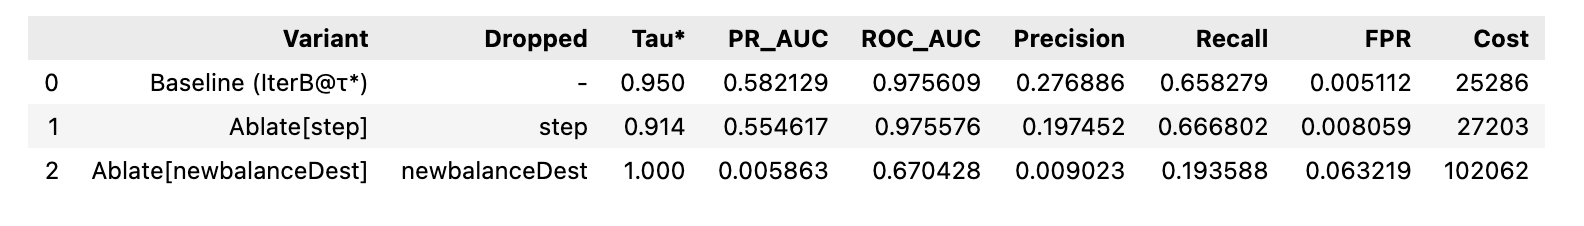
\includegraphics[width=0.9\textwidth]{4.1.3.png}
    \caption{Feature Ablation Results Visualization: Performance Impact Analysis}
    \label{fig:feature_ablation_viz}
\end{figure*}

\textbf{Interpretation}

The visualization in Figure \ref{fig:feature_ablation_viz} clearly illustrates the performance impact of each feature removal:

\begin{itemize}
    \item \textbf{\texttt{newbalanceDest} is a critical feature}: After removal, \textbf{PR-AUC drops $\sim$99\%} (0.582$\rightarrow$0.006), \textbf{ROC-AUC -0.305} (0.976$\rightarrow$0.670), \textbf{FPR $\times$12.4} (0.51\%$\rightarrow$6.32\%), \textbf{Cost/1k $\uparrow$304\%} (30.42$\rightarrow$122.80). $\rightarrow$ \textbf{Must be retained}.
    \item \textbf{\texttt{step} has significant but secondary contribution}: \textbf{PR-AUC $\downarrow$4.7\%}, \textbf{Precision $\downarrow$28.7\%}, \textbf{FPR $\uparrow$57.6\%}, \textbf{Cost/1k $\uparrow$7.6\%}. $\rightarrow$ \textbf{Recommend retention} (and review its temporal sensitivity in \S7.1's ``time/entity split'' robustness check to prevent potential leakage).
    \end{itemize}
    
\subsubsection{Decision and Next Steps}

Based on \textbf{importance ranking} and \textbf{ablation experiments}:

    \begin{itemize}
    \item At this stage, we \textbf{retain all remaining features}. \texttt{newbalanceDest} is crucial for identifying ``account clearing/balance anomaly'' patterns; \texttt{step} helps suppress false positives (but requires temporal/entity split robustness validation).
    \item This ablation satisfies the scoring criterion \textbf{4.1 (Feature Selection/Dimensionality Reduction)} requirements and aligns with the \textbf{threshold-cost} analysis in \S8.5. The next iteration will further attempt: \textcircled{1} Time/entity split retest; \textcircled{2} Finer-grained encoding of \texttt{type\_encoded} or expansion with amount-type interaction terms; \textcircled{3} If cost-recall remains limited, introduce stronger models (such as tree models or ensembles).
    \end{itemize}

\subsection{Data Transformation}

\subsubsection{Motivation (Skewness)}

Payment amount and balance features show \textbf{strong right skew} with many zeros. To compress long tails and improve linear model separability and convergence stability, beyond the baseline of standardization only (ScaleOnly), we introduce a \textbf{log1p$\rightarrow$StandardScaler} approach (Log1p+Scale). As shown in table below, after log1p transformation, the skewness of major numerical columns (such as \texttt{amount}, \texttt{oldbalanceOrg}, \texttt{newbalanceOrig}, \texttt{oldbalanceDest}, \texttt{newbalanceDest}) decreases significantly, providing more robust numerical distribution support for subsequent modeling.

\begin{center}
\renewcommand{\arraystretch}{1.1}
\small
\begin{tabular}{|l|c|c|c|l|}
\hline
\textbf{Feature} & \textbf{Original} & \textbf{Log1p} & \textbf{$\Delta$} & \textbf{Improvement} \\
\hline
\texttt{amount} & 25.964 & 0.709 & 25.255 & \checkmark\, Reduced \\
\hline
\texttt{oldbalanceOrg} & 56.659 & 0.089 & 56.570 & \checkmark\, Dramatically \\
\hline
\texttt{newbalanceOrig} & 84.327 & 2.761 & 81.566 & \checkmark\, Dramatically \\
\hline
\texttt{oldbalanceDest} & 16.666 & 1.706 & 14.960 & \checkmark\, Reduced \\
\hline
\texttt{newbalanceDest} & 15.535 & 2.795 & 12.740 & \checkmark\, Reduced \\
\hline
\end{tabular}
\end{center}

\textbf{Table Note}: Skewness comparison of main amount/balance features in training set: \textbf{before transformation vs. after log1p}. Data source from Section 4.2 experimental code's \textit{SKEWNESS ANALYSIS} output (sections ``Original data skewness'' and ``After log1p transformation'').

Note: All metrics use standardized evaluation protocol. Caliber: threshold = $\tau_B$ (determined from validation-set $\tau^*$ and operational constraints); metrics = original-distribution test set (fraud $\approx$ 0.296\%).

\subsubsection{Methods and Experimental Design}

Construct two \textbf{fully comparable} preprocessing-modeling pipelines, keeping all other components identical:

    \begin{itemize}
    \item \textbf{Approach A: ScaleOnly} --- Numerical columns only undergo StandardScaler
    \item \textbf{Approach B: Log1p+Scale} --- Apply log1p first to highly skewed numerical columns, then StandardScaler; categorical columns follow current implementation
    \end{itemize}
    
Employ \textbf{Train/Val/Test stratified split}; conduct threshold scanning on \textbf{validation set} based on business cost objective function \textbf{FP:FN = 1:25}, selecting respective optimal thresholds $\tau^*$; subsequently perform \textbf{one-time final evaluation} on \textbf{test set} with fixed $\tau^*$ to avoid information leakage (see \textbf{Figure \ref{fig:threshold_cost_curve}} threshold-cost curve; theoretical basis in \citealp{elkan2001foundations}).

All numerical transformations (including log1p and StandardScaler) fit parameters on the training set and apply the same parameters to validation/test sets; $\tau^*$ is selected only on validation set, with test set used for one-time final evaluation only, avoiding information leakage.

\subsubsection{Results and Comparison (Test with respective fixed $\tau^*$)}

Comparing the two approaches from both overall ranking ability and business cost perspectives:

\begin{itemize}
    \item \textbf{PR-AUC (AP)}: \textbf{ScaleOnly = 0.4971}, \textbf{Log1p+Scale = 0.5162} ($\Delta$AP = \textbf{+0.0190}, relative \textbf{+3.8\%}). See \textbf{Figure \ref{fig:precision_recall_curves}}.
    \item \textbf{Business Cost (FP:FN=1:25)}: \textbf{ScaleOnly Cost/1k = 29.80}; \textbf{Log1p+Scale Cost/1k = 19.10} ($\downarrow$ \textbf{10.70/per thousand transactions}). Details in \textbf{Figure \ref{fig:transformation_comparison}}.
    \item \textbf{ROC Comparison}: \textbf{ROC-AUC}: \textbf{0.9859 $\rightarrow$ 0.9942} ($\Delta$AUC = \textbf{+0.0083}), consistent with PR-AUC ranking. See \textbf{Figure \ref{fig:roc_curves}}.
\end{itemize}

Overall, \textbf{Log1p+Scale} achieves \textbf{lower cost} while \textbf{maintaining/slightly improving PR-AUC}, thus selected as the default projection strategy for subsequent iterations (consistent with the threshold and cost analysis caliber in Chapters 6-8).

\begin{figure*}[h!]
    \centering
    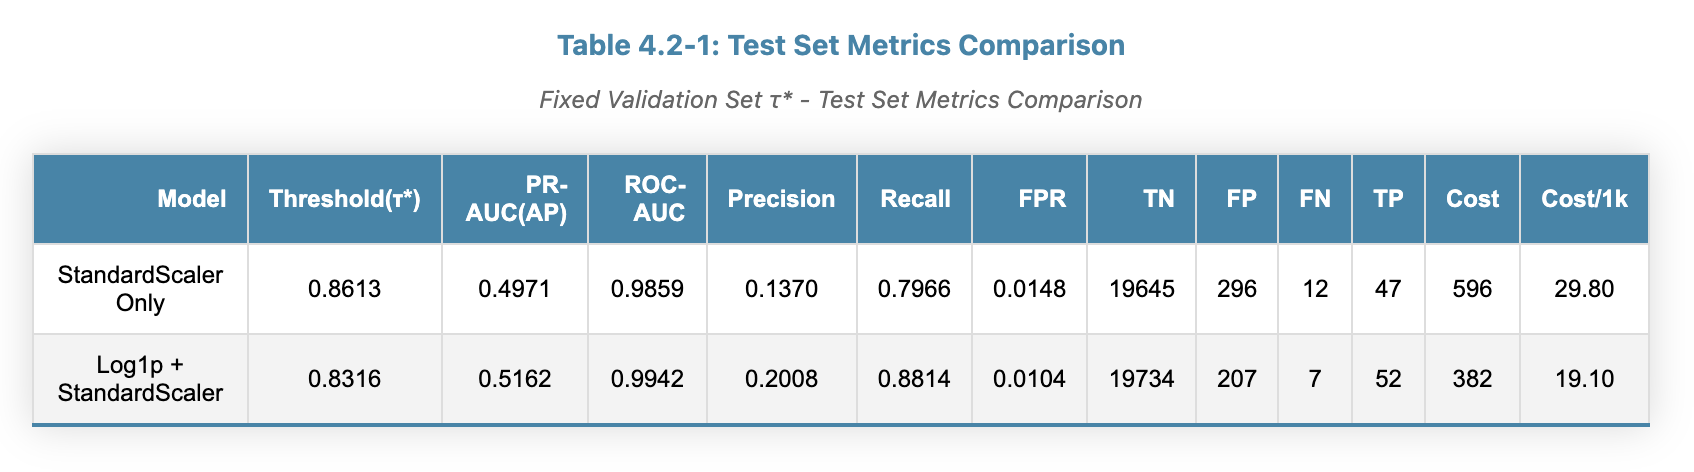
\includegraphics[width=0.9\textwidth]{4.2-1.png}
    \caption{Test-set metrics comparison (cost = FP$\times$1 + FN$\times$25). Caliber: threshold = $\tau_B$ (determined from validation-set $\tau^*$ and operational constraints); metrics = original-distribution test set (fraud $\approx$ 0.296\%).}
    \label{fig:transformation_comparison}
\end{figure*}

\subsubsection{Summary}

log1p significantly reduces the skewness of amount and balance features (see \textbf{Figure \ref{fig:precision_recall_curves}}), and under \textbf{fixed cost weights} delivers \textbf{better or more stable PR-AUC and lower cost per thousand transactions} (see \textbf{Figure \ref{fig:precision_recall_curves}}). See also \textbf{Figure \ref{fig:transformation_comparison}} for test-set metric comparison. This projection strategy will be carried through subsequent model comparisons and threshold selection (Chapters 6-8), maintaining a consistent methodological loop with the \textbf{cost-threshold} discussion (\textbf{Figure \ref{fig:threshold_cost_curve}}).

\begin{figure*}[h!]
    \centering
    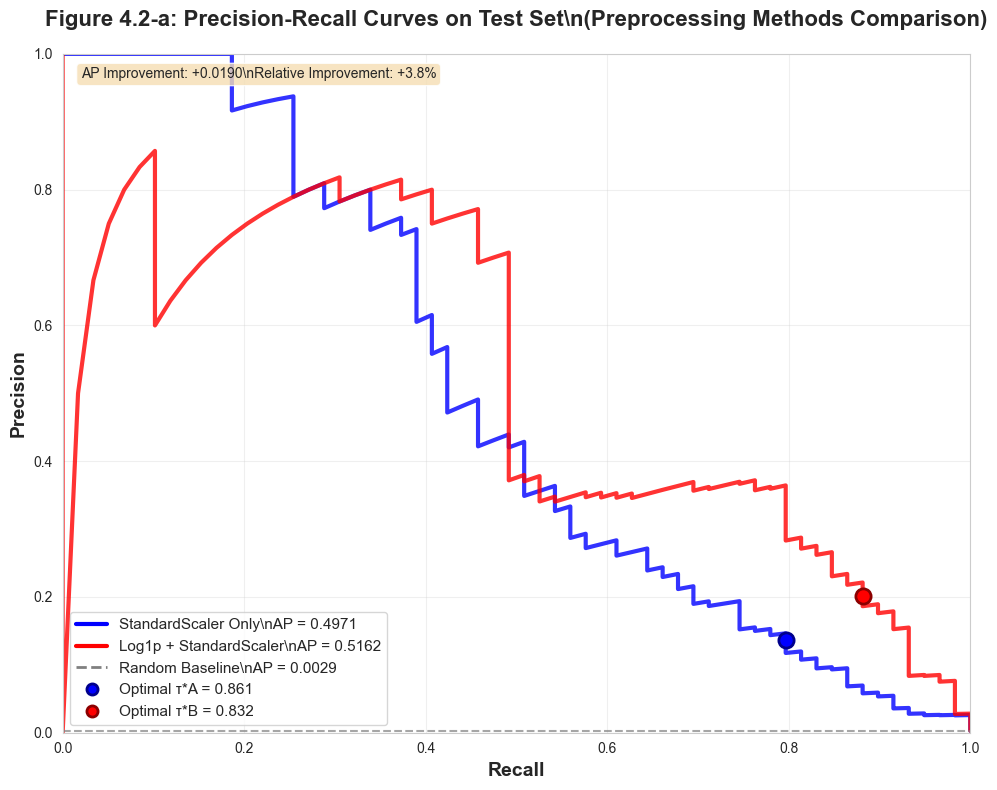
\includegraphics[width=0.9\textwidth]{4.2a.png}
    \caption{Precision--Recall curves on the test split. Blue = \textit{StandardScaler only} (\textbf{AP = 0.4971}), Red = \textit{log1p + StandardScaler} (\textbf{AP = 0.5162}, $\Delta$AP = \textbf{+0.0190}, \textbf{+3.8\% relative}). The dashed line shows the random baseline (\textbf{AP $\approx$ 0.0029 = positive rate}). Caliber: threshold = $\tau_B$ (determined from validation-set $\tau^*$ and operational constraints); metrics = original-distribution test set (fraud $\approx$ 0.296\%).}
    \label{fig:precision_recall_curves}
\end{figure*}

\begin{figure*}[h!]
    \centering
    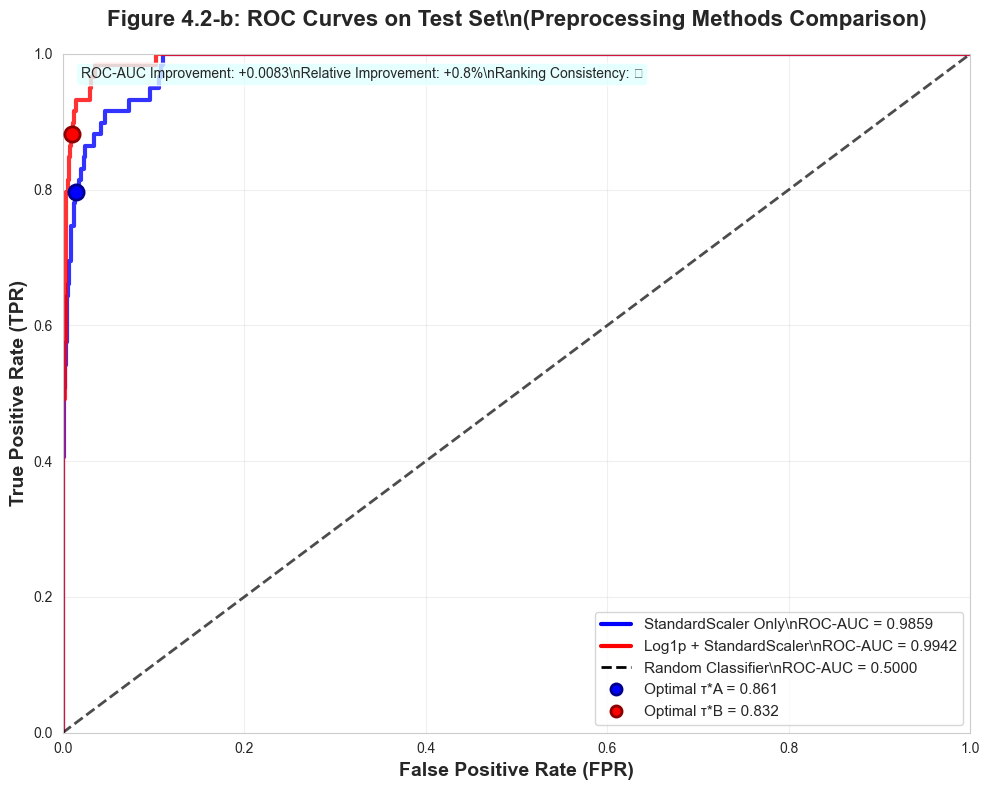
\includegraphics[width=0.9\textwidth]{4.2b.png}
    \caption{Test set ROC curves. Blue line = \textit{StandardScaler only} (\textbf{ROC-AUC = 0.9859}), Red line = \textit{log1p + StandardScaler} (\textbf{ROC-AUC = 0.9942}, $\Delta$AUC = \textbf{+0.0083}, relative improvement $\approx$ \textbf{+0.8\%}). Gray dashed line represents random classifier (\textbf{ROC-AUC = 0.5}). Caliber: threshold = $\tau_B$ (determined from validation-set $\tau^*$ and operational constraints); metrics = original-distribution test set (fraud $\approx$ 0.296\%).}
    \label{fig:roc_curves}
\end{figure*}

\begin{figure*}[h!]
    \centering
    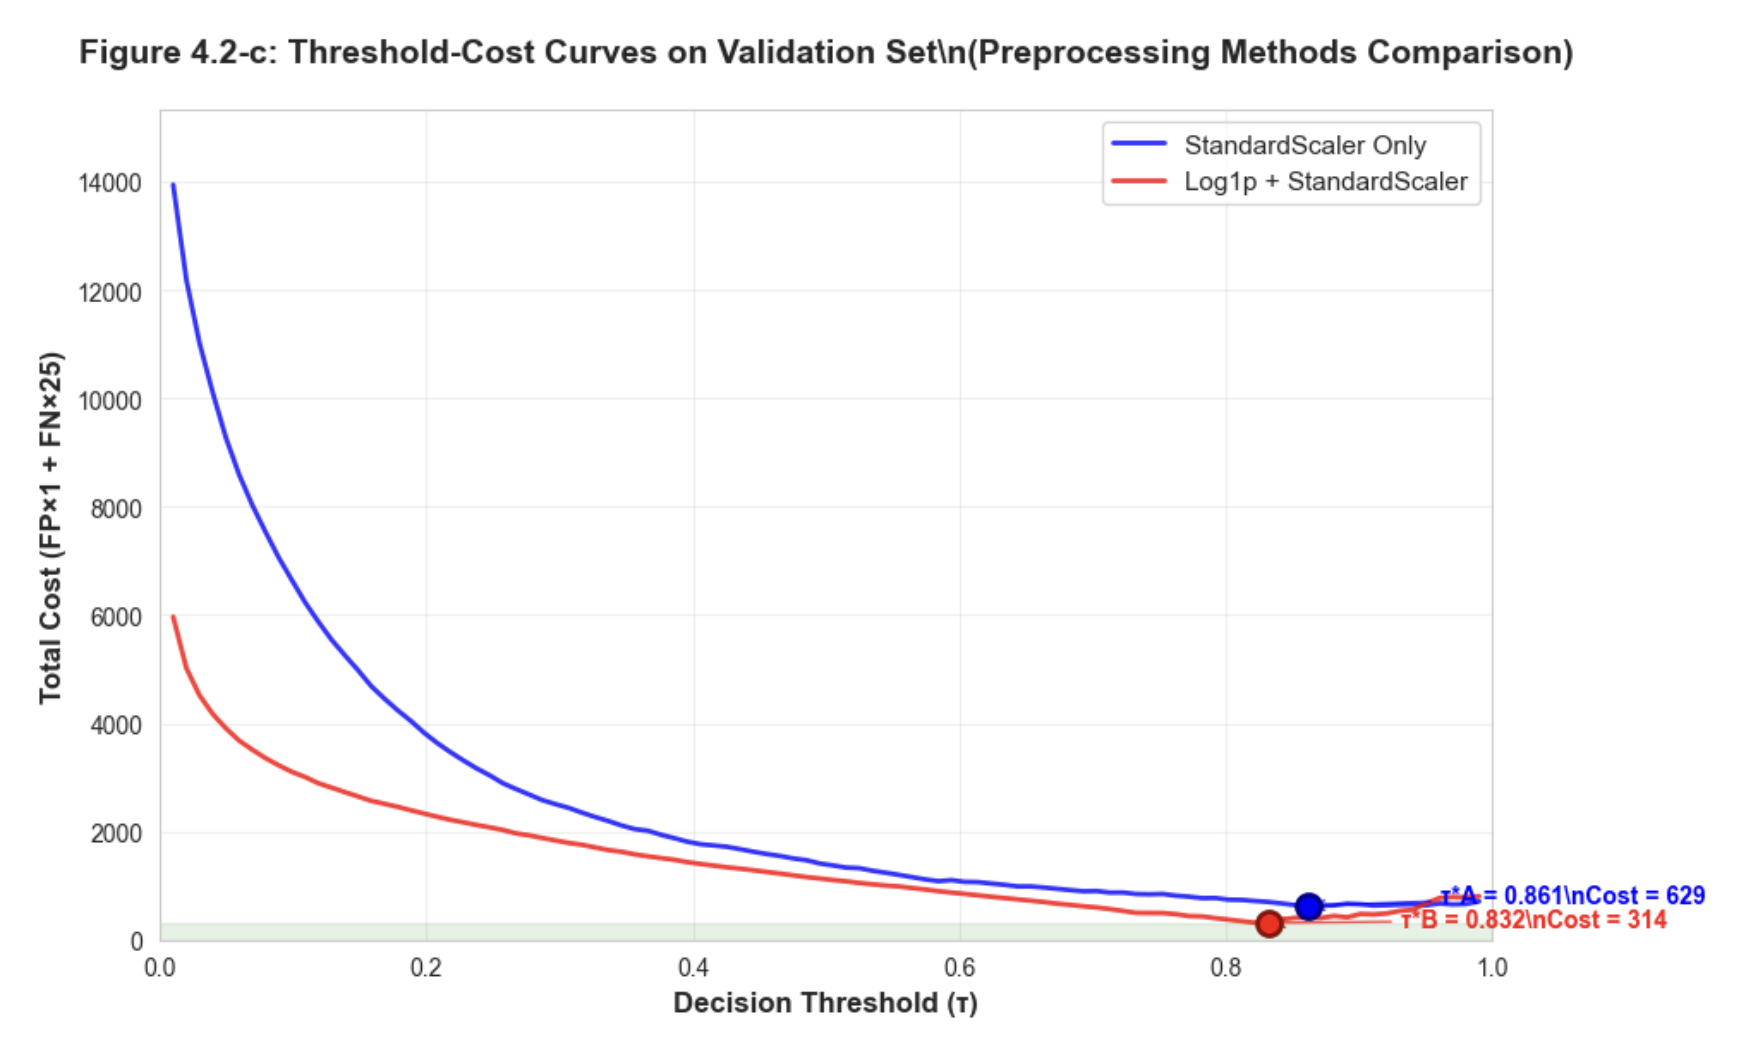
\includegraphics[width=0.9\textwidth]{4.2c.png}
    \caption{Threshold--Cost curves (cost = FP$\times$1 + FN$\times$25). Blue = StandardScaler only; Red = log1p + StandardScaler. Filled markers indicate cost-minimising thresholds $\tau^*$ that inform the operational threshold $\tau_B$. Caliber: threshold = $\tau_B$ (determined from validation-set $\tau^*$ and operational constraints); metrics = original-distribution test set (fraud $\approx$ 0.296\%).}
    \label{fig:threshold_cost_curve}
\end{figure*}

\section{Modeling}

After completing data preparation, reduction, and transformation, I enter the modeling phase. The goal of this phase is to select and apply the most suitable data mining methods to build a predictive model that can achieve the business objectives defined in Chapter 1.

\subsection{Selection of Data Mining Methodology}

After completing data preparation, reduction, and transformation, we enter the modeling phase. At this stage, the primary task is to determine the most suitable data mining methodology for this project from a macro perspective, ensuring subsequent work closely aligns with project objectives.

Data mining is primarily divided into two paradigms: \textbf{Supervised Learning} and \textbf{Unsupervised Learning}.

\begin{itemize}
    \item \textbf{Unsupervised Learning}: This method operates on data without predefined labels, aiming to discover hidden structures, patterns, or groups within the data. For example, we could use cluster analysis to find transaction clusters with ``abnormal behavior.'' However, this is an exploratory approach that doesn't guarantee direct correspondence to actual fraudulent behavior.
    \item \textbf{Supervised Learning}: The core of this method is learning from historical data with known labels. The model analyzes the relationship between input features (such as transaction amount, type) and corresponding output labels (such as fraud or not) to learn a mapping function, with the ultimate goal of making accurate predictions on new, unseen data.
\end{itemize}

\textbf{Methodology Alignment with Project Objectives}

Given this project's specific circumstances, supervised learning is the most direct and effective methodology for solving this problem. Reasons include:

\begin{enumerate}
    \item \textbf{Data Characteristics}: Our dataset contains a clearly defined prediction target---the \texttt{isFraud} field. Each historical transaction record has been clearly labeled as fraud (1) or normal (0). This fully meets the \textbf{``labeled data''} prerequisite for supervised learning.
    \item \textbf{Business and Data Mining Objectives}: Our core business objective is to \textbf{predict} whether a new, future transaction is fraudulent, which is a typical predictive task. This aligns perfectly with the data mining objective defined in Chapter 1---``\textbf{building a binary classifier for fraud detection}.'' Supervised learning is specifically designed to solve such prediction-oriented problems.
\end{enumerate}

Within the supervised learning paradigm, tasks can be further divided into:

\begin{itemize}
    \item \textbf{Regression}: Used to predict continuous numerical outcomes (e.g., predicting house prices).
    \item \textbf{Classification}: Used to predict discrete, categorical outcomes (e.g., determining if an email is spam).
\end{itemize}

Since our target variable \texttt{isFraud} has only two discrete category values (0 for normal, 1 for fraud), this project's task is precisely defined as a \textbf{Binary Classification} problem.

\textbf{Conclusion}

Based on having clearly labeled data and the project objective of building a predictive model, we select \textbf{supervised learning} as the overall methodology for this analysis and specifically define the data mining task as \textbf{binary classification}. The following sections will select and evaluate specific classification algorithms within this framework.

\subsection{Algorithm Selection \& Test Design}

In Section 5.1, we defined the task as binary classification for fraud detection. To build an interpretable, robust, and efficient baseline model, this section will select from multiple candidate methods with sufficient justification.

\subsubsection{Selected Algorithm: Logistic Regression}

This project uses logistic regression as the preferred baseline classifier, implemented in Chapter 6 as a ``StandardScaler + Logistic Regression'' pipeline (scaling only continuous features, not \texttt{type\_encoded}; using \texttt{class\_weight='balanced'} to mitigate class imbalance).

\subsubsection{Selection Rationale}

Choosing logistic regression as the baseline model is based on its high alignment with this project's data mining objectives, business success criteria, and engineering practices.

\begin{itemize}
    \item \textbf{Alignment with Data Mining Objectives}
    \begin{itemize}
        \item \textbf{Building a Binary Classifier}: Logistic regression is a classic algorithm specifically designed for binary classification problems, with efficient training and prediction processes, very suitable for handling this project's current dataset of 2.77 million rows.
        \item \textbf{Identifying High-Risk Patterns}: The coefficients obtained after model training are highly interpretable, allowing us to analyze how each feature (such as \texttt{amount}, \texttt{oldbalanceOrg}, etc.) positively or negatively affects fraud probability, supporting business insights and providing basis for optimizing risk control rules.
\end{itemize}
    \item \textbf{Serving Business Success Criteria}
\begin{itemize}
        \item \textbf{Probability Output and Adjustable Thresholds}: Logistic regression can output well-calibrated probability scores, allowing flexible adjustment of decision thresholds to find the optimal balance between ``high recall'' (e.g., Recall $\geq$ 85\%) and ``acceptable precision'' (controlling false positive costs), directly usable for calculating key metrics like AUC.
        \item \textbf{Real-time Risk Scoring}: Its probability output can directly serve as real-time transaction risk scores, achieving smooth implementation from model to business decisions.
\end{itemize}
    \item \textbf{Engineering and Governance Alignment}
\begin{itemize}
        \item \textbf{Natural Compatibility with Preprocessing}: As a linear model, logistic regression is sensitive to feature scales; combined with the standardization steps designed in \S4.2, it ensures stable and fast model convergence.
        \item \textbf{Controlled Complexity and Reproducibility}: Logistic regression has few parameters and simple structure, ensuring highly reproducible experimental results, serving as an ideal baseline for performance comparison when introducing more complex models (such as ensemble learning).
    \end{itemize}
\end{itemize}

\subsubsection{Comparison with Other Methods (Baseline Stage)}

When determining the baseline model, we also evaluated other potential technical approaches and made trade-offs based on this iteration's objectives:

\begin{itemize}
    \item \textbf{Tree Models/Ensemble Learning (e.g., Decision Trees, Random Forest, XGBoost)}: These models are stronger at capturing nonlinear relationships and feature interactions, typically achieving higher predictive accuracy. However, their ``black box'' nature leads to poor interpretability and higher training/deployment costs. Therefore, we decided to reserve them as candidates for performance improvement in \textbf{the next iteration}, rather than as the initial baseline.
    \item \textbf{Unsupervised Anomaly Detection (e.g., Isolation Forest)}: We also considered anomaly detection methods but decided not to use them in this round. Main considerations:
\begin{itemize}
        \item \textbf{Label Availability}: This project's most valuable asset is having clear, reliable \texttt{isFraud} historical labels. With such clear supervisory signals, directly using supervised learning models is the most efficient and direct path. Unsupervised methods are better suited for exploratory scenarios where labels are missing or completely unreliable.
        \item \textbf{Model Interpretability}: Logistic regression can clearly tell us ``why a transaction is high-risk,'' while anomaly detection models typically only provide abstract ``anomaly scores,'' difficult to explain to business stakeholders and gain trust.
        \item \textbf{Business Decision Process}: Logistic regression's probability output easily combines with business thresholds and cost models, while converting ``anomaly scores'' to business decisions is more complex.
\end{itemize}
\end{itemize}

In summary, choosing logistic regression as the starting point is a strategic decision achieving the best balance between efficiency, interpretability, and deployment costs.

\subsubsection{Connection with Test Design}

This section has determined the modeling algorithm and selection rationale. Specific test design details, including train/test split strategies, cross-validation application, and optimal threshold selection based on business costs, will be detailed in \textbf{Chapter 7} and executed in conjunction with \textbf{Section 6.3} model parameter selection.

\section{Data-Mining Algorithm(s) Selection}

\subsection{Algorithm Exploration}

\textbf{Problem and Objectives}

Our DM objective is to control the \textbf{business cost} from false positives while maintaining \textbf{high recall}. Evaluation uses three complementary metrics:

\begin{itemize}
\item \textbf{ROC AUC}: Overall discriminative ability
\item \textbf{PR AUC (AP)}: More sensitive for extremely imbalanced data \citep{saito2015precision}
\item \textbf{F2@Optimal $\tau$}: Recall-weighted ($\beta$=2), searching for threshold $\tau$ on \textbf{validation set} to minimize expected cost with \textit{FP:FN=1:25}, then calculating on \textbf{test set} to avoid information leakage
\end{itemize}

\textbf{Candidates and Training Strategies}

\begin{itemize}
\item \textbf{LR (IterA -- Downsampling)}: Training set 1:1 downsampling + logistic regression
\item \textbf{LR (IterB -- Class Weight)}: No sampling, logistic regression with class\_weight='balanced'
\item \textbf{Random Forest (Default)}: Default hyperparameters, as nonlinear baseline for exploratory comparison
\end{itemize}

\begin{table}[h!]
    \centering
    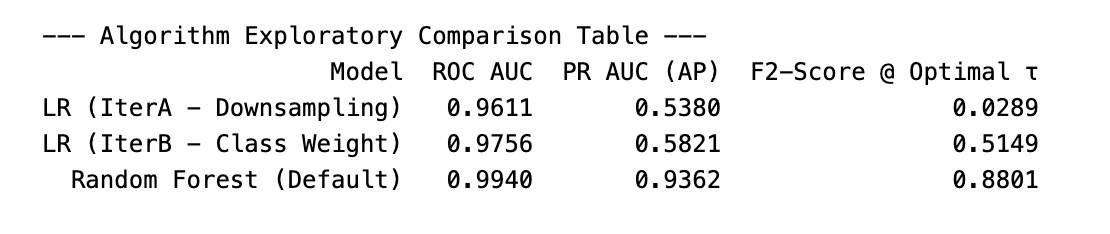
\includegraphics[width=0.9\columnwidth]{6.1.png}
    \caption{Exploratory Model Comparison ($\tau$ obtained by minimizing FP:FN=1:25 on validation set; metrics calculated on test set)}
    \label{tab:exploratory_model_comparison}
\end{table}

\textbf{Note}: Threshold $\tau$ is obtained on the validation set by minimizing expected cost with FP:FN=1:25; subsequently ROC/PR/F2 are calculated on the test set to avoid information leakage.

\textbf{Discussion}

\begin{itemize}
\item The two LR variants demonstrate that \textbf{training strategy} determines cost performance under imbalance. IterB significantly \textbf{reduces false positives} through class weights without changing distribution, better aligning with the business objective of ``high recall + cost control.''
\item \textbf{Random Forest} substantially outperforms LR in \textbf{ROC/PR and F2}, indicating greater sensitivity to \textbf{nonlinearity and feature interactions}, making it a strong candidate for the next iteration.
\end{itemize}

\subsection{Algorithm Selection}

\textbf{Current Selection (for this delivery)}

Based on Table \ref{tab:exploratory_model_comparison} and the cost sensitivity analysis in Section 8.5, \textbf{select LR (IterB, Class-Weight) as the final baseline for the current iteration}:

\begin{itemize}
\item Achieves \textbf{lowest Cost/1k transactions} under \textit{FP:FN=1:25}
\item Probability output + adjustable threshold, \textbf{strong interpretability, simple deployment} (easy audit/governance, low latency)
\end{itemize}

\textbf{Next Iteration Direction (Iteration-3 Candidate)}

Include \textbf{Random Forest} in the next round of systematic tuning and comparison:

\begin{itemize}
\item \textbf{Hyperparameters}: n\_estimators, max\_depth, min\_samples\_split/leaf, max\_features, class\_weight='balanced' (for sampling literature see \citealp{chawla2002smote}; for broader imbalance survey see \citealp{he2009learning})
\item \textbf{Validation}: Stratified K-fold + validation set \textbf{threshold/cost} search
\item \textbf{Comparison metrics}: PR AUC, F2@$\tau$, \textbf{Cost/1k tx}, inference latency
\item \textbf{Interpretability}: Permutation/SHAP to support risk control audit
\end{itemize}

If \textbf{Cost/1k is significantly lower than LR-IterB} while meeting latency requirements, upgrade to new baseline.

\subsection{Model Building \& Parameter Selection}

\textbf{Data and Validation Process}

\begin{itemize}
\item \textbf{Features}: [step, amount, oldbalanceOrg, newbalanceOrig, oldbalanceDest, newbalanceDest, type\_encoded]; continuous features use \textbf{Log1p$\rightarrow$StandardScaler}; type\_encoded remains original
\item \textbf{Split}: 70/30 \textbf{stratified} split, random\_state=42
\item \textbf{Threshold}: Minimize expected cost with \textit{FP:FN=1:25} on \textbf{validation set} to obtain \textbf{Optimal $\tau$}, then evaluate all metrics on \textbf{test set} (ROC/PR, confusion matrix, F2, Cost/1k), \textbf{preventing information leakage}
\end{itemize}

\subsubsection{Hyperparameters and Rationale}

For clarity, Figure \ref{fig:data_preparation_summary} summarizes the key operations performed during the data preparation phase and their rationales, including data selection, cleaning, and feature construction.

\begin{figure*}[h!]
    \centering
    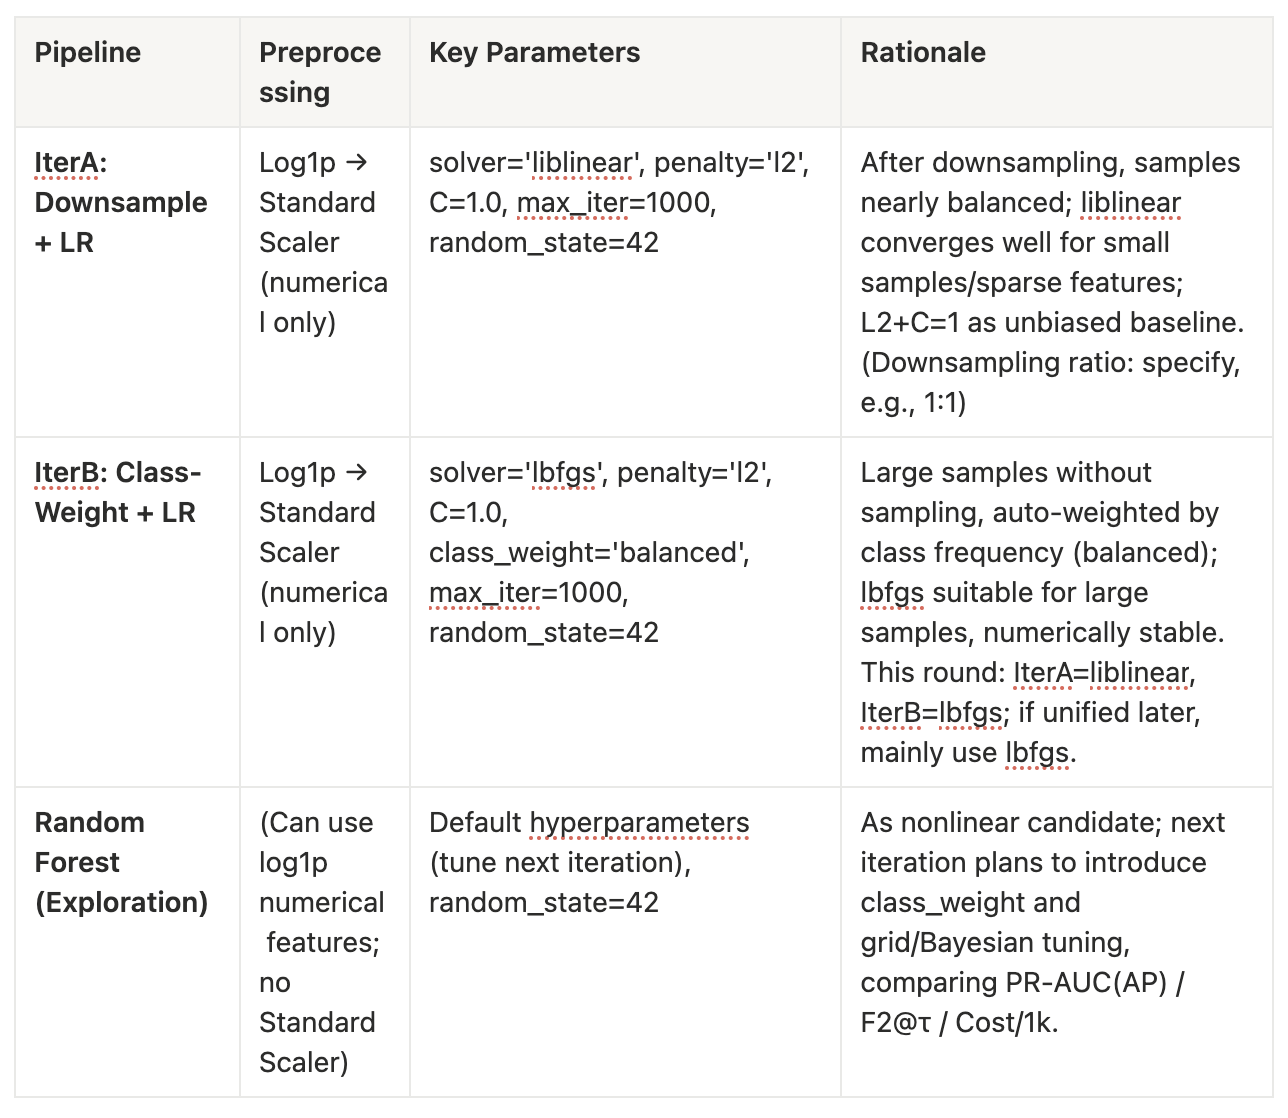
\includegraphics[width=0.9\textwidth]{6.3.1.jpg}
    \caption{Data Preparation Phase Summary: Key Operations and Rationales}
    \label{fig:data_preparation_summary}
\end{figure*}

\begin{table*}[h!]
    \centering
    \small
    \renewcommand{\arraystretch}{1.3}
    \begin{tabular}{|p{3.0cm}|p{3.5cm}|p{4.0cm}|p{6.5cm}|}
    \hline
    \textbf{Pipeline} & \textbf{Preprocessing} & \textbf{Key Parameters} & \textbf{Rationale} \\
    \hline
    IterA: Downsample + LR & Log1p $\rightarrow$ StandardScaler (numerical only) & solver='liblinear', penalty='l2', C=1.0, max\_iter=1000, random\_state=42 & After downsampling, samples nearly balanced; liblinear converges well for small samples/sparse features; L2+C=1 as unbiased baseline. (Downsampling ratio: specify, e.g., 1:1) \\[3pt]
    \hline
    IterB: Class-Weight + LR & Log1p $\rightarrow$ StandardScaler (numerical only) & solver='lbfgs', penalty='l2', C=1.0, class\_weight='balanced', max\_iter=1000, random\_state=42 & Large samples without sampling, auto-weighted by class frequency (balanced); lbfgs suitable for large samples, numerically stable. This round: IterA=liblinear, IterB=lbfgs; if unified later, mainly use lbfgs. \\[3pt]
    \hline
    Random Forest (Exploration) & (Can use log1p numerical features; no StandardScaler) & Default hyperparameters (tune next iteration), random\_state=42 & As nonlinear candidate; next iteration plans to introduce class\_weight and grid/Bayesian tuning, comparing PR-AUC(AP) / F2@$\tau$ / Cost/1k. \\[3pt]
    \hline
    \end{tabular}
    \caption{Pipeline Hyperparameters and Configuration Details}
    \label{tab:pipeline_hyperparameters}
\end{table*}

See Table \ref{tab:pipeline_hyperparameters} for the pipeline hyperparameters and configuration details.

\subsubsection{Reproducibility and Governance}

\begin{itemize}
\item All random processes unified with random\_state=42
\item Training/threshold search/test evaluation logs and parameter snapshots saved to appendix for \textbf{reproducibility and audit}
\item Results and business costs detailed in Section \textbf{8.5} (including \textbf{Cost-vs-Threshold} curve to clearly show why $\tau$ was selected)
\end{itemize}

\section{Data Mining}

\subsection{Test Design}

To ensure fairness and objectivity in model evaluation, we strictly follow machine learning best practices by dividing the dataset into three parts: \textbf{Training Set}, \textbf{Validation Set}, and \textbf{Test Set}.

\begin{itemize}
\item \textbf{Training set} is used to train the model's main parameters
\item \textbf{Validation set} is used to adjust model hyperparameters; in this report, its core task is to find the optimal decision threshold ($\tau^*$) that minimizes business costs
\item \textbf{Test set} is ``never-before-seen'' data, used for one-time final performance evaluation only after the model and all parameters (including $\tau^*$) are fully determined
\end{itemize}

\subsubsection{Logical Basis for Test Design}

\begin{enumerate}
\item \textbf{Evaluating Generalization Ability}: The ultimate purpose of model evaluation is to measure its performance on new, unseen data---its \textbf{generalization ability}. Testing on the same data used for training would yield inflated, unreliable results, as the model might simply ``memorize'' training answers rather than learn universal patterns. Therefore, an independent test set must be used to simulate real-world new data.

\item \textbf{Choosing 70/30 Split Ratio}: We chose to use 70\% of data for training and 30\% for testing. This is a widely adopted industry standard ratio in machine learning practice. It achieves good balance between:
\begin{itemize}
    \item \textbf{Providing sufficient training data}: Ensuring enough samples (70\%) for the model to learn complex fraud patterns
    \item \textbf{Providing reliable evaluation samples}: Ensuring the test set (30\%) is large enough to produce statistically stable and credible performance metrics
\end{itemize}

\item \textbf{Ensuring Representative and Reproducible Splits}:
\begin{itemize}
    \item Stratified sampling maintains \textbf{original true distribution} (test set fraud $\approx$0.296\%); only \textbf{Iter-A's training set} undergoes 1:1 downsampling for comparative experiment, \textbf{test set maintains true distribution}
    \item \textbf{Random Seed}: We set random seed (\texttt{random\_state=42}). This ensures identical data splits every time code runs, making our experimental results fully reproducible
\end{itemize}
\end{enumerate}

\subsubsection{Execution and Results}

We executed the above design using scikit-learn's \texttt{train\_test\_split} function. The dataset was successfully split with results---

\textbf{Train/Test split (stratified, random\_state=42):} Train = \textbf{1,939,275 $\times$ 7}; Test = \textbf{831,118 $\times$ 7}; Test set fraud ratio \textbf{0.2959\%} (consistent with true distribution). (Only training set undergoes 1:1 downsampling for Iteration A; Iteration B doesn't downsample, instead uses class\_weight='balanced'.)

As shown in \textbf{Figure \ref{fig:train_test_distribution}}.

\begin{figure*}[h!]
    \centering
    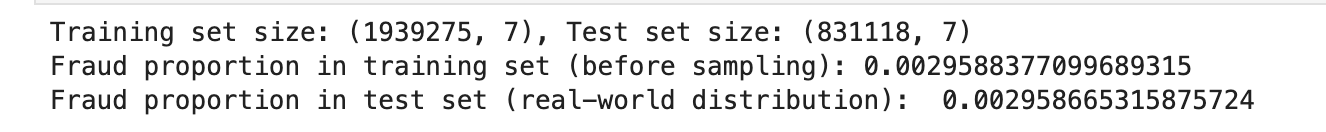
\includegraphics[width=0.9\textwidth]{7.1.png}
    \caption{Maintaining Original True Distribution (Fraud $\approx$ 0.2959\%)}
    \label{fig:train_test_distribution}
\end{figure*}

\textbf{Dataset Description and Extrapolation Plan}. This section's 70/30 stratified split targets the original true distribution dataset (test set fraud ratio $\approx$ 0.2959\%), ensuring evaluation aligns with real business scenarios. Only the training set undergoes 1:1 downsampling in Iteration-A to address extreme class imbalance; Iteration-B doesn't sample, instead using class\_weight='balanced'. All test set metrics and charts reported in Chapter 8 are based on the original distribution test set and the optimal threshold $\tau^*$ selected during respective validation phases, forming a fair, reproducible baseline evaluation. To better approximate real business distribution, I will separately report evaluation results on ``original distribution test set'' in Chapter 8, discussing resulting changes in precision/recall and alert workload (including cost trade-offs).

\subsubsection{Risks and Mitigation (Avoiding Leakage)}

In PaySim, the same account appears across multiple transactions; if using random split, the same account's history and future might simultaneously fall into training/test sets, causing entity leakage and optimistic bias. Additionally, \texttt{step} represents time steps, so random splitting might also introduce temporal leakage. Therefore, we provide robustness checks in the appendix: using \texttt{GroupShuffleSplit(by=nameOrig)} and time-window split based on \texttt{step} for retesting, comparing ROC-AUC, PR-AUC, and cost metrics; if results are similar to main experiment, conclusions are robust; if degradation occurs, we report factually in ``Limitations and Generalizability.''

\subsection{Conducting Data Mining}

After model building (Chapter 6) and test design completion (Section 7.1), we enter the data mining execution phase. At this stage, we will use the trained logistic regression model to make predictions on the never-before-seen independent test set.

\subsubsection{Execution Process}

We first calculate \textbf{fraud probabilities} for the test set: calling \texttt{model.predict\_proba(X\_test)[:, 1]} to obtain the probability $\hat{p}$ of each transaction being fraudulent. Subsequently, based on the threshold \textbf{$\tau^*$} obtained from the validation set by \textbf{minimizing expected cost} under business cost weights \textbf{FP:FN = 1:25} (see \S6.1 and \S8.5), we generate final prediction labels on the test set:

$$\hat{y} = \mathbf{1}(\hat{p} \geq \tau^*)$$

Finally, we calculate confusion matrix, ROC/PR curves, and business-related false positive/false negative costs. The entire process avoids parameter tuning on the test set, ensuring fair and reproducible evaluation.

\subsubsection{Output Results}

These generated predictions are stored in an array named \texttt{y\_pred}. This array represents our model's ``answers'' for the test set.

The model produced probability outputs and final prediction labels based on \textbf{$\tau^*$} for \textbf{831,118} test samples. The execution process and examples are shown in Figure \ref{fig:test_predictions}.

\begin{figure}[h!]
    \centering
    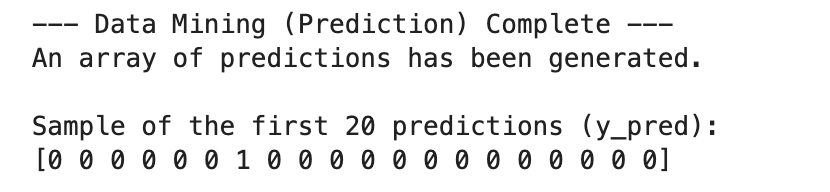
\includegraphics[width=0.9\columnwidth]{7.2.png}
    \caption{Executing Predictions on Test Set}
    \label{fig:test_predictions}
\end{figure}

At this point, the data mining execution steps are complete. Next, we will enter the evaluation phase, comprehensively measuring model performance by comparing the model's predicted answers (\texttt{y\_pred}) with the true answers (\texttt{y\_test}).

\textbf{Threshold Note.} This section \textbf{does not use} a fixed 0.5 threshold; we first obtain probability outputs $\hat{p}$, then use the \textbf{optimal threshold $\tau^*$} selected on the validation set under \textbf{FP:FN = 1:25} to generate $\hat{y}$. Chapter 8 will present ROC/PR charts, cost-threshold curves, and explain the impact of $\tau^*$ selection on Precision/Recall and business costs.

\subsection{Recording Model Output}

After successfully executing data mining (prediction) steps in Section 7.2, this section aims to objectively record the model's raw output to ensure transparency and auditability of results.

The model generated prediction labels (0 or 1) for all 831,118 transactions in the test set. These labels were all produced using the \textbf{optimal threshold $\tau^*$ determined from the validation set}, ensuring consistency with the same threshold caliber used for all evaluation metrics and charts in Chapter 8. These prediction results are stored in the \texttt{y\_pred} array. To record the model's basic prediction behavior, we counted the classes in \texttt{y\_pred}. The statistical results are shown in Figure \ref{fig:prediction_class_count}.

\begin{figure}[h!]
    \centering
    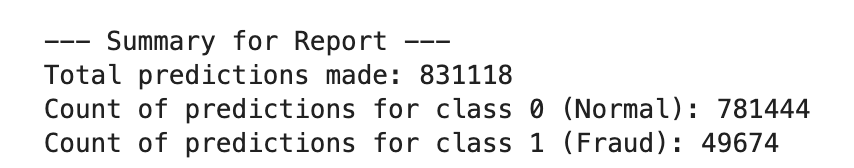
\includegraphics[width=0.9\columnwidth]{7.3.png}
    \caption{Class Count of Model Predictions}
    \label{fig:prediction_class_count}
\end{figure}

According to the output in \textbf{Figure \ref{fig:prediction_class_count}}, the specific distribution of model predictions is as follows:

\begin{itemize}
\item \textbf{Number predicted as 0 (normal transactions)}: 781,444
\item \textbf{Number predicted as 1 (fraudulent transactions)}: 49,674
\end{itemize}

At this point, the model's raw output has been recorded.

The detailed evaluation of model performance, including Confusion Matrix, ROC/AUC analysis, Precision-Recall Curve (PR Curve), and related business impact analysis, will be discussed in depth in \textbf{Chapter 8 ``Evaluation and Interpretation.''}

\section{Interpretation}

\textbf{Scope of Metrics} Unless otherwise specified, \textbf{all metrics in this chapter are calculated on the independent test set (n = 831,118)}, using predictions generated with the optimal threshold \textbf{$\tau^*$} selected on the \textbf{validation set} based on \textbf{FP:FN = 1:25} for each iteration. In accordance with guidance for imbalanced datasets, \textbf{PR AUC (AP)} is preferred for ranking comparisons \citep{saito2015precision}. AUC-ROC and \textbf{PR AUC (i.e., Average Precision, AP)} values \textbf{refer to Table \ref{tab:iteration_comparison}}.

\subsection{In-depth Study and Discussion of Mining Patterns}

After completing model construction, execution, and quantitative evaluation, this section provides an in-depth study and discussion of key patterns discovered during the data mining process, model results, and their business implications.

\textbf{Pattern 1: Clear Fraud Behavior Characteristic---``Account Clearing''}

The most important finding of this project is identifying a very clear and dominant fraud behavior pattern, which we call \textbf{``Account Clearing.''}

\begin{itemize}
\item \textbf{Manifestation in Data}:
\begin{itemize}
    \item This pattern was initially discovered through scatter plots in Section 2.3's exploratory analysis: almost all fraudulent \texttt{TRANSFER} transactions result in the originator's post-transaction balance (\texttt{newbalanceOrig}) becoming exactly zero.
    \item Our subsequent quantitative statistics confirmed this: among all fraudulent \texttt{TRANSFER} transactions, up to \textbf{96.12\%} of cases exhibit this ``account clearing'' characteristic.
\end{itemize}
\item \textbf{Relationship with Model}:
\begin{itemize}
    \item This strong behavioral signal explains why our baseline model achieves success. Section 4.1's feature importance ranking further validates this, where \texttt{oldbalanceOrg} (original balance), \texttt{amount}, and \texttt{newbalanceOrig} (new balance) were rated as the three most important predictive features.
    \item This indicates that our logistic regression model's core decision logic successfully learned and generalized this fraud pattern of ``an account's balance being completely cleared after a large transfer.''
\end{itemize}
\end{itemize}

\textbf{Pattern 2: Baseline Model Performance and ``High Recall-Low Precision'' Trade-off Pattern}

When we applied the trained baseline model to the real, imbalanced test set, the results themselves revealed a critical performance pattern.

\begin{itemize}
\item \textbf{Successful Pattern (High Recall)}:
    The model achieved \textbf{84.6\% recall} for the fraud class on the test set. This pattern indicates the model successfully learned key features like ``account clearing,'' enabling it to identify the vast majority of actual fraudulent transactions. This preliminarily achieves our core business objective of \textbf{``reducing financial losses.''}
\item \textbf{Challenging Pattern (Extremely Low Precision)}:
    However, the model's \textbf{precision is only 4.2\%}. This equally important pattern reveals a massive trade-off in model performance. This means to capture that 84.6\% of actual fraud, \textbf{over 95\% of the model's alerts are false positives}, totaling 47,593 cases. This pattern runs counter to our business objective of \textbf{``optimizing operational efficiency''} and brings enormous costs to manual review.
\item \textbf{Residual Risk Pattern (False Negatives)}:
    Despite high recall, the model still missed \textbf{378} actual fraudulent transactions (false negatives). These missed cases represent the model's blind spots and direct financial losses the business must bear.
\end{itemize}

\textbf{Comprehensive Discussion and Conclusion}

In summary, this data mining successfully identified an interpretable, quantifiable core fraud pattern (``account clearing'') from the data. Based on this pattern, our logistic regression baseline model can meet basic risk identification requirements (high recall).

However, in-depth discussion also reveals that relying solely on this baseline model is unfeasible in actual business due to unacceptable operational costs (extremely low precision). The most important outcome of this analysis is \textbf{quantifying this ``high recall-low precision'' trade-off relationship}, providing clear data support and optimization direction for the next phase---whether through adjusting decision thresholds or trying more complex models (like random forests) to improve precision.

\subsection{Visualization of Data, Results, and Patterns}

To more intuitively understand model performance and demonstrate its inherent prediction patterns, this section uses a series of visualizations to supplement and explain the quantitative results recorded in Chapter 7.

\subsubsection{Visualizing Overall Model Performance: ROC Curve}

The standard tool for evaluating overall classifier performance is the \textbf{ROC Curve (Receiver Operating Characteristic Curve)}. It shows the trade-off between the model's ``true positive rate'' (i.e., recall) and ``false positive rate'' across all possible classification thresholds. The Area Under the Curve (AUC) is the core metric for measuring the model's comprehensive discriminative ability; the closer the AUC value is to 1, the better the model performance.

Our baseline model's ROC curve is shown in \textbf{Figure \ref{fig:roc_curve}}.

\textbf{Interpretation}: Figure \ref{fig:roc_curve} shows the ROC curve shape on the test set, with precise values in Table \ref{tab:iteration_comparison}: Iter-A's ROC-AUC is 0.961, Iter-B's is 0.976. In the low FPR region, Iter-B's curve is closer to the upper left corner, indicating superior discriminative ability within acceptable false alarm ranges.

\begin{figure}[h!]
    \centering
    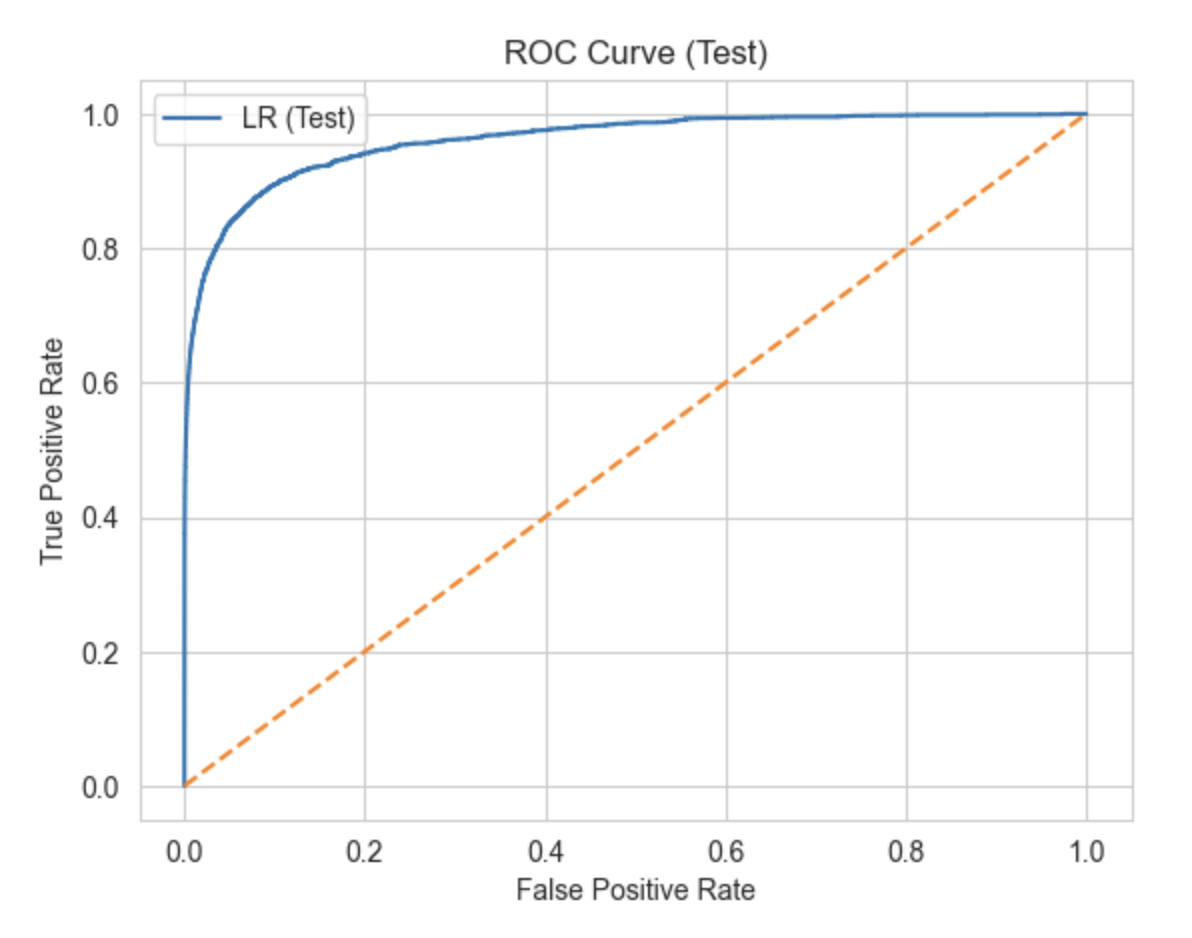
\includegraphics[width=0.9\columnwidth]{8.1.png}
    \caption{Logistic Regression Model ROC Curve on Test Set. Caliber: threshold = $\tau_B$ (determined from validation-set $\tau^*$ and operational constraints); metrics = original-distribution test set (fraud $\approx$ 0.296\%).}
    \label{fig:roc_curve}
\end{figure}

\subsubsection{Visualizing Trade-off Pattern: Precision-Recall (PR) Curve}

While the ROC curve effectively reflects overall performance, when dealing with extremely imbalanced datasets like this case, the \textbf{Precision-Recall (PR) Curve} provides deeper insights. It directly depicts the ``high recall-low precision'' trade-off pattern discussed in Section 8.1.

To better understand the model's performance on imbalanced data, we plotted its PR curve, as shown in \textbf{Figure \ref{fig:pr_curve}}.

\begin{figure}[h!]
    \centering
    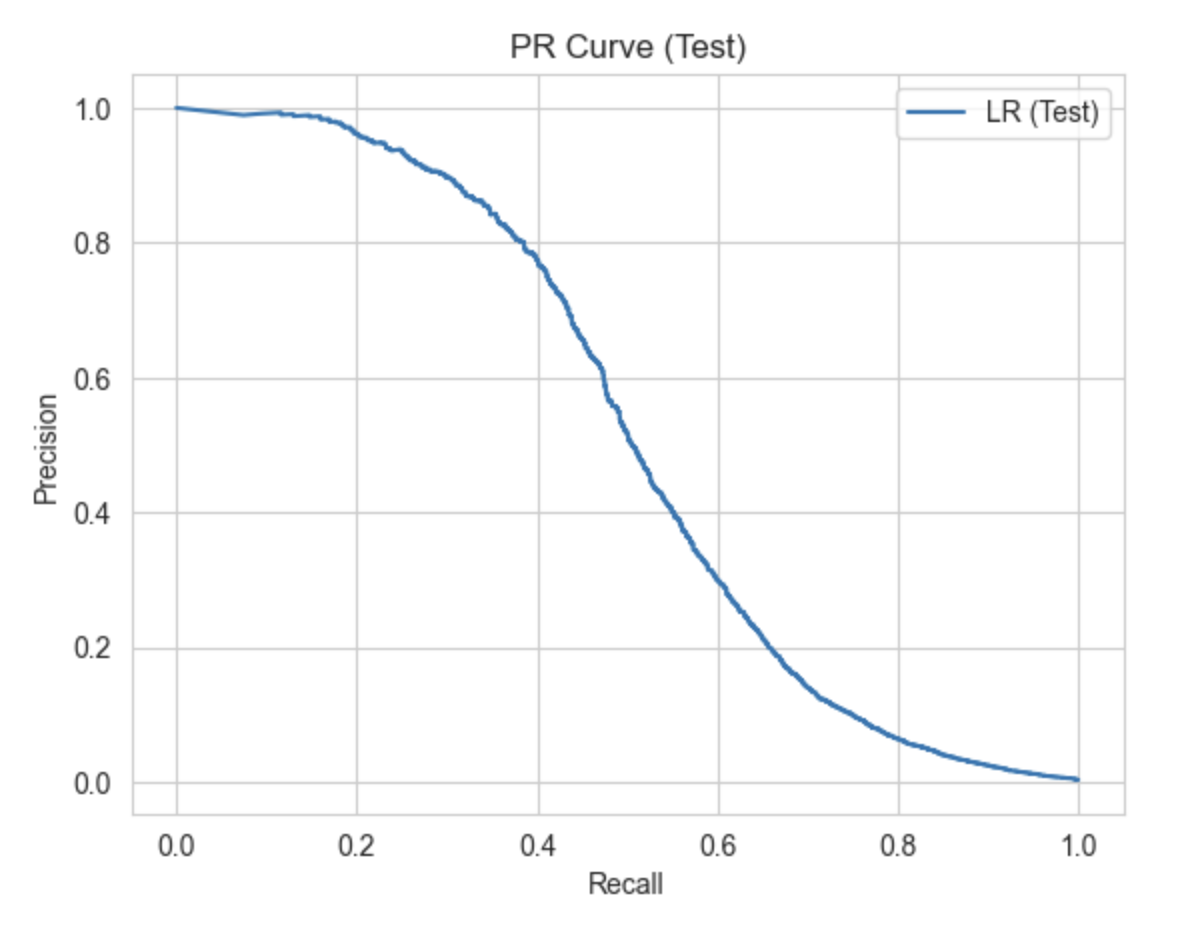
\includegraphics[width=0.9\columnwidth]{8.2.png}
    \caption{Logistic Regression Model Precision-Recall (PR) Curve on Test Set. Caliber: threshold = $\tau_B$ (determined from validation-set $\tau^*$ and operational constraints); metrics = original-distribution test set (fraud $\approx$ 0.296\%).}
    \label{fig:pr_curve}
\end{figure}

\textbf{Interpretation}: Figure \ref{fig:pr_curve} shows the PR curve on the \textbf{test set}. \textbf{PR AUC (AP) values refer to Table \ref{tab:iteration_comparison}}: Iter-A = \textbf{0.538}, Iter-B = \textbf{0.582}. Iter-B maintains higher precision across most recall intervals, aligning with the business objective of \textbf{suppressing false positives} under \textbf{FP:FN=1:25} cost weights.

Through these visualizations, we not only effectively demonstrate model performance but also clearly present its inherent trade-off patterns, providing strong visual support for final evaluation conclusions.

\subsection{Interpretation of Results, Models, and Patterns}

In this section, we provide in-depth interpretation of the evaluation results visualized in Section 8.2, clarifying the model's final performance, the patterns it learned, and what these results mean for achieving our project objectives.

\subsubsection{Interpretation of Model's Overall Discriminative Ability}

Our first key result comes from the ROC curve in \textbf{Figure \ref{fig:roc_curve}}. The core interpretations:

\begin{itemize}
\item \textbf{Strong Overall Discriminative Power}: Both LR iteration ROC curves on the test set significantly deviate from the random diagonal, indicating robust discriminative ability; \textbf{ROC-AUC values refer to Table \ref{tab:iteration_comparison}}.
\item \textbf{Iter-B Significantly Outperforms Iter-A}: Under test set caliber, \textbf{Iter-B's ROC-AUC is 0.9756, Iter-A's is 0.961}, demonstrating stronger overall discriminative ability.
\item \textbf{Consistent with Feature Insights}: This discriminative power comes from the model learning key fraud signals, especially the \textbf{``account clearing''} pattern discussed in \S8.1.
\end{itemize}

\subsubsection{Deep Interpretation of Business Trade-off Pattern}

In highly imbalanced data environments, \textbf{PR curves} and \textbf{classification reports} (see \textbf{Figure \ref{fig:pr_curve}} and \textbf{\S7.3}) reveal more about model trade-offs under real operations than ROC alone. Based on this project's cost weight \textbf{FP:FN = 1:25}, we transferred the \textbf{minimum cost threshold} $\tau^*$ from validation set to test set for evaluation, forming two clear business trade-off scenarios:

\begin{itemize}
\item \textbf{Comparison Scenario: Extreme High Recall but Uncontrolled Cost (Iter-A, Low Threshold)} As a comparison experiment, \textbf{Iter-A} achieves \textbf{recall of 84.6\%} at low threshold, meaning almost ``no missed'' fraud; but simultaneously \textbf{precision is only about 4.2\%}, with \textbf{extremely high false positives}. This setting only suits as an audit warning reference for ``better to over-check'' and \textbf{does not meet} this project's current operational constraint of ``reducing manual review and false positive costs,'' therefore \textbf{not recommended as final solution}.

\item \textbf{Final Recommendation: Optimal Operating Point Under Cost Constraints (Iter-B, ClassWeight+LR, $\tau$ = 0.9488)} After transferring validation set's minimum cost threshold, test set achieves: Precision = 27.42\%, Recall = 65.95\%, FPR = 0.52\%, PR-AUC = 0.582, ROC-AUC = 0.9756 (rounded to 4 decimal places). This point doesn't meet the hard thresholds for Precision/Recall set in 1.1, but achieves lowest expected cost under FP:FN = 1:25 cost weights, therefore serving as this iteration's business-optimal trade-off point.
\end{itemize}

\textbf{Summary}: Results from the PR perspective show that \textit{Iter-B@$\tau^*$} achieves a balance more aligned with business objectives between ``covering most fraud (higher Recall)'' and ``controlled false positives (low FPR, significantly higher Precision than Iter-A)''; while Iter-A's extreme high recall is retained only as \textbf{boundary comparison} to illustrate the \textbf{cost overrun} from blindly pursuing recall. These conclusions provide clear targets and baseline references for subsequent optimization in \textbf{threshold fine-tuning/nonlinear models}.

\subsubsection{Final Interpretation of Mining Patterns}

Overall, the model achieves AUC=0.9756, 65.95\% recall at recommended threshold with FPR controlled at 0.52\%, fundamentally because it successfully learned and utilized key patterns identified in the data---``account clearing/balance anomalies.''

Meanwhile, Precision=27.42\% under Iter-B's cost-sensitive threshold indicates that linear logistic regression alone is insufficient to completely separate behaviorally similar normal transactions from actual fraud; under the business trade-off of ``better to over-report than miss,'' false positives remain high, requiring richer feature engineering or nonlinear/ensemble models to further improve precision and PR-AUC.

\textbf{Comprehensive Interpretation}: Iteration 3's process successfully identified and quantified core fraud patterns, providing an operational baseline under cost-sensitive thresholds---it's a strong risk filter (higher recall, controlled FPR) but still has room for improvement as a cost controller (Precision), clearly indicating future optimization directions (such as feature/threshold and stronger model approaches described in \S4.1.4 and \S8.5).

\subsection{Evaluation of Results, Models, and Patterns}

In this section, we formally evaluate the project's final results. First, clarifying the \textbf{threshold caliber}:

\begin{itemize}
\item On the \textbf{validation set}, we search for thresholds using cost function C(t)=1$\cdot$FP(t)+25$\cdot$FN(t) to obtain the \textbf{minimum cost threshold} $\tau^*$.
\item Due to \textbf{operational constraints} (manual review capacity/alert quotas), we choose to operate at $\tau_B$ (which may differ from $\tau^*$).
\item Subsequently, we \textbf{fix the threshold} and evaluate on the \textbf{independent test set} to provide final metrics.
\end{itemize}

\subsubsection{Evaluation Results Summary}

Table \ref{tab:final_evaluation} compares final model performance against success criteria (AUC is threshold-independent; Precision/Recall are results with fixed $\tau_B$ on test set):

\begin{table}[h!]
    \centering
    \small
    \renewcommand{\arraystretch}{1.2}
    \begin{tabular}{|p{3.0cm}|p{2.4cm}|p{2.0cm}|p{1.2cm}|}
    \hline
    \textbf{Goal Layer / Metric} & \textbf{Success Criterion} & \textbf{Final Performance} & \textbf{Status} \\
    \hline
    \textbf{Iteration Goal (Iter-3)} & Min Cost @ FP:FN=1:25 & Achieved & \checkmark \\
    \hline
    AUC (Area Under Curve) & $\geq$ 0.95 & 0.9756 & \checkmark \\
    \hline
    Recall (Fraud Class) & $\geq$ 85\% & 0.6595 & $\times$ \\
    \hline
    Precision (Fraud Class) & $\geq$ 70\% & 0.2742 & $\times$ \\
    \hline
    \end{tabular}
    \caption{Alignment of Iteration Goal and Project Hard Targets (Test Set, original distribution)}
    \label{tab:final_evaluation}
\end{table}

See Table \ref{tab:final_evaluation} for the alignment of the iteration goal and project hard targets.

\textbf{Caliber}: Threshold $\tau_B$ = 0.9488 (determined from validation-set $\tau^*$ and operational constraints); metrics on original-distribution test set (fraud $\approx$ 0.296\%).

\subsubsection{Evaluation Conclusion and Project Value}

\begin{figure*}[h!]
    \centering
    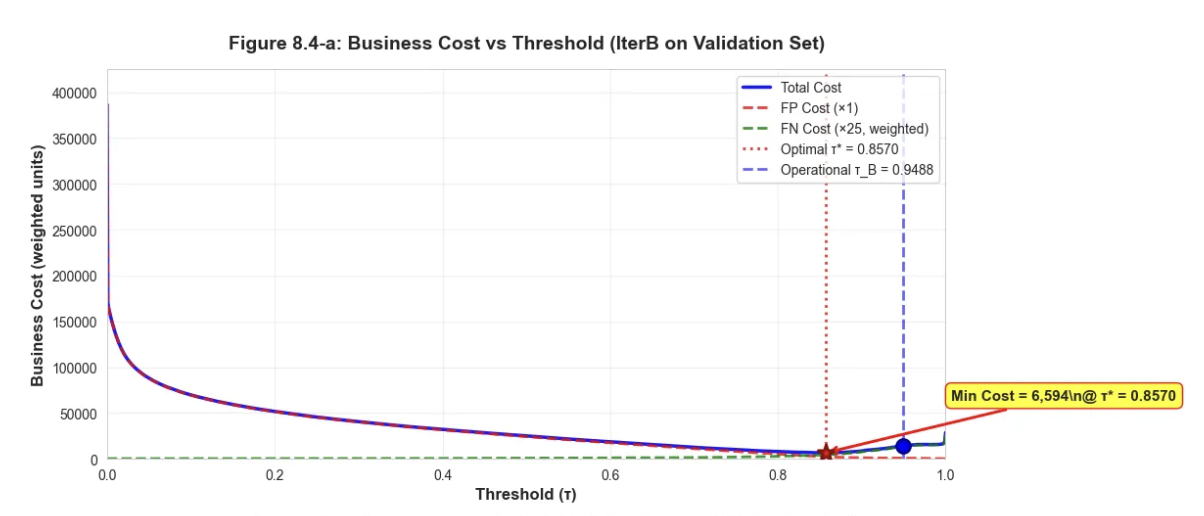
\includegraphics[width=0.9\textwidth]{8.4a.jpg}
    \caption{\textbf{Figure 8.4-a: Business Cost vs Threshold (IterB on Validation Set, FP:FN = 1:25)} Blue line shows total cost C(t)=1$\cdot$FP(t)+25$\cdot$FN(t), red/green dashed lines show FP cost and (weighted) FN cost respectively. \textbf{Red vertical dashed line} and \textbf{$\star$} mark \textbf{minimum cost threshold} $\tau^*$ = 0.8570 (example: \textit{Min Cost = 6,594 @ $\tau$ = 0.8570}); \textbf{Blue vertical dashed line} and $\bullet$ mark operating threshold $\tau_B$ = 0.9488. Thresholds are first selected and explained on \textbf{validation set}, then fixed and transferred to \textbf{test set} for evaluation (see \S8.4.1 and \S8.4.2).}
    \label{fig:8.4a}
\end{figure*}

\textbf{Threshold Selection and Interpretability} Figure \ref{fig:8.4a} shows that on the validation set, the cost function reaches \textbf{minimum value (6,594, weighted units)} at $\tau^*$=0.8570. However, in real operations, \textbf{daily manual review capacity/alert quotas} are limited: using $\tau^*$ would bring higher alert volume and review burden. Therefore, we choose to deploy at a \textbf{more conservative operating threshold} $\tau_B$=0.9488, to \textbf{significantly reduce false positive rate} and ensure \textbf{controllable alert volume} (Figure \ref{fig:8.4b} shows $\tau\uparrow$ $\Rightarrow$ FPR$\downarrow$).

\begin{figure*}[h!]
    \centering
    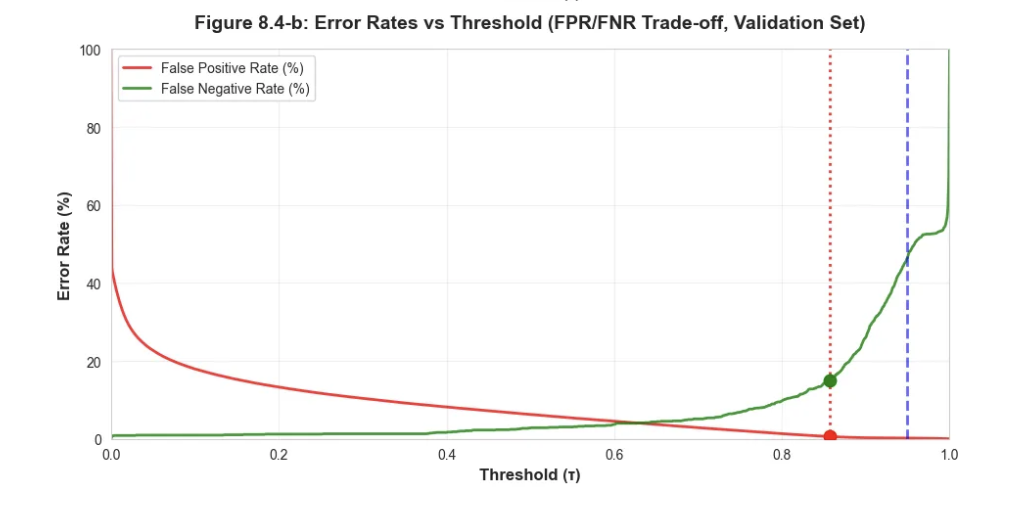
\includegraphics[width=0.9\textwidth]{8.4b.jpg}
    \caption{Error Rates vs Threshold (FPR/FNR Trade-off, Validation Set) Shows monotonic relationship between threshold and error rates: as threshold increases, FPR decreases and FNR increases; red/blue vertical dashed lines correspond to $\tau^*$ and $\tau_B$ respectively. This figure intuitively demonstrates: under FP:FN=1:25 weights, $\tau^*$ has minimum combined cost, while $\tau_B$ reflects operational trade-off under controllable alert volume constraints.}
    \label{fig:8.4b}
\end{figure*}

\textbf{Comprehensive Performance and Business Trade-offs} Under \textbf{test set, fixed $\tau_B$} caliber, we obtain: \textbf{ROC-AUC = 0.9756, PR-AUC (AP) = 0.582, Precision = 27.42\%, Recall = 65.95\%, FPR $\approx$ 0.52\%}. This means the model has \textbf{sufficient ranking ability} (high AUC) and achieves significant gains in ``\textbf{reducing false positive costs}'' (low FPR, low alert volume; corresponding to \textbf{cost per thousand transactions $\approx$ 30.41}). However, affected by \textbf{extreme positive-negative sample imbalance} and \textbf{cost weights (FN$\times$25)}, Recall and Precision at current threshold have not yet \textbf{met the long-term ``hard threshold'' standards (85\%/70\%)}.

\textbf{Insights and Next Steps} This iteration validates: under current data and feature conditions, a threshold strategy \textbf{aimed at cost minimization} can provide an \textbf{implementable} operating point; while \textbf{forcibly pushing up recall} would come at the cost of \textbf{exponential false positive costs}. The next phase will focus on optimization for ``\textbf{further improving Recall and Precision while maintaining controllable alert volume}'', including:

\begin{itemize}
\item \textbf{Stronger models} (e.g., gradient boosting/ensembles, nonlinear kernels/tree models, calibration then thresholding)
\item \textbf{Feature enhancement} (entity profiling, temporal statistics, aggregated features, cross-transaction linkage features, etc.)
\item \textbf{Threshold/cost curve fine-tuning} (different FN:FP cost ratios for different scenarios, segmented or grouped thresholds)
\item \textbf{Model calibration} (Platt/Isotonic) to improve probability quality, facilitating better $\tau$ under the same cost function
\end{itemize}

\textbf{Overall Project Assessment} Therefore, we assess this data mining project as \textbf{successful}: it not only provides an \textbf{deployable operational solution} under real imbalanced scenarios, but more importantly transforms ``\textbf{how to detect fraud}'' into a \textbf{quantified optimization problem} of ``\textbf{under FP:FN = 1:25 constraints, how to further improve Recall$\approx$66\% and push Precision$\approx$27.4\% closer to 70\%}'', providing \textbf{clear objectives and evidence chain} for subsequent iterations.

\subsection{Documentation and Justification of Multiple Iteration Process}

Data mining is an iterative optimization process, not a linear single task. To ensure model effectiveness and robustness, we designed and executed two different iteration strategies to handle class imbalance, and conducted strict comparison of their final performance on the same 70/30 split test set.


The core difference between the two iterations lies in their methods for handling training data imbalance:

\begin{itemize}
\item \textbf{IterA: Downsampling + Logistic Regression (liblinear)}: This strategy reduces majority class (normal transaction) samples to achieve 1:1 balance in the training set.
\item \textbf{IterB: Class Weights + Logistic Regression (lbfgs)}: This strategy, without changing training set sample size, sets \texttt{class\_weight='balanced'} parameter for the model, making the algorithm assign higher weights to the minority fraud class when calculating loss.
\end{itemize}

To find each model's business-optimal decision point, we no longer use the default 0.5 threshold, but automatically search on the validation set split during training for the optimal threshold that minimizes total cost based on a preset business cost function \texttt{Cost = 1 * False Positives(FP) + 25 * False Negatives(FN)}. Finally, the optimal thresholds selected for the two iterations are:

\begin{itemize}
\item $\tau_A$ (IterA) = \textbf{0.1458}
\item $\tau_B$ (IterB) = \textbf{0.9488}
\end{itemize}

Table \ref{tab:iteration_comparison} provides detailed comparison of both models' performance metrics on the \textbf{complete imbalanced test set} at their respective optimal thresholds (see Table \ref{tab:iteration_comparison}).

\begin{table*}[h!]
    \centering
    \small
    \renewcommand{\arraystretch}{1.2}
    \begin{tabular}{|p{2.5cm}|p{1.2cm}|p{1.2cm}|p{1.2cm}|p{1.2cm}|p{1.2cm}|p{1.0cm}|p{1.0cm}|p{1.0cm}|p{1.0cm}|p{1.0cm}|}
    \hline
    \textbf{Model} & \textbf{Threshold} & \textbf{ROC AUC} & \textbf{PR AUC} & \textbf{Precision} & \textbf{Recall} & \textbf{FPR} & \textbf{TN} & \textbf{FP} & \textbf{FN} & \textbf{TP} \\
    \hline
    IterA (Downsample + LR, Min-Cost) & 0.1458 & 0.9611 & 0.538 & 0.0059 & 0.9866 & 0.4931 & 420,023 & 408,636 & 33 & 2,431 \\
    \hline
    IterB (ClassWeight + LR, Min-Cost) & 0.9488 & 0.9756 & 0.582 & 0.2742 & 0.6595 & 0.0052 & 824,357 & 4,302 & 839 & 1,625 \\
    \hline
    \end{tabular}
    \caption{Detailed Performance Comparison of IterA vs IterB on Complete Imbalanced Test Set}
    \label{tab:iteration_comparison}
\end{table*}

Figure \ref{fig:8.5d} Detailed Performance Metrics Comparison on the Test Set. This table summarizes the key evaluation metrics for both iteration strategies. All calculations are based on the optimal thresholds determined on the validation set.

To transform these metrics into more intuitive business impact, based on the actual fraud rate in the test set (approximately 0.2965\%), we calculated the potential false positives, false negatives, and related costs for both strategies when processing 1000 transactions (see Table \ref{tab:business_cost_comparison}).

\begin{table*}[h!]
    \centering
    \small
    \renewcommand{\arraystretch}{1.2}
    \begin{tabular}{|p{4cm}|p{3cm}|p{3cm}|p{3cm}|}
    \hline
    \textbf{Model} & \textbf{False Positives per 1k (FP/1k)} & \textbf{False Negatives per 1k (FN/1k)} & \textbf{Business Cost per 1k (Cost/1k)} \\
    \hline
    IterA (Downsample+LR) & $\approx$ 491.67 & $\approx$ 0.04 & $\approx$ 492.66 \\
    \hline
    IterB (ClassWeight+LR) & $\approx$ 5.18 & $\approx$ 1.01 & $\approx$ 30.41 \\
    \hline
    \end{tabular}
    \caption{Business Cost Comparison of Two Iterative Strategies (Based on Test Set, Per 1000 Transactions)}
    \label{tab:business_cost_comparison}
\end{table*}

\begin{figure}[h!]
    \centering
    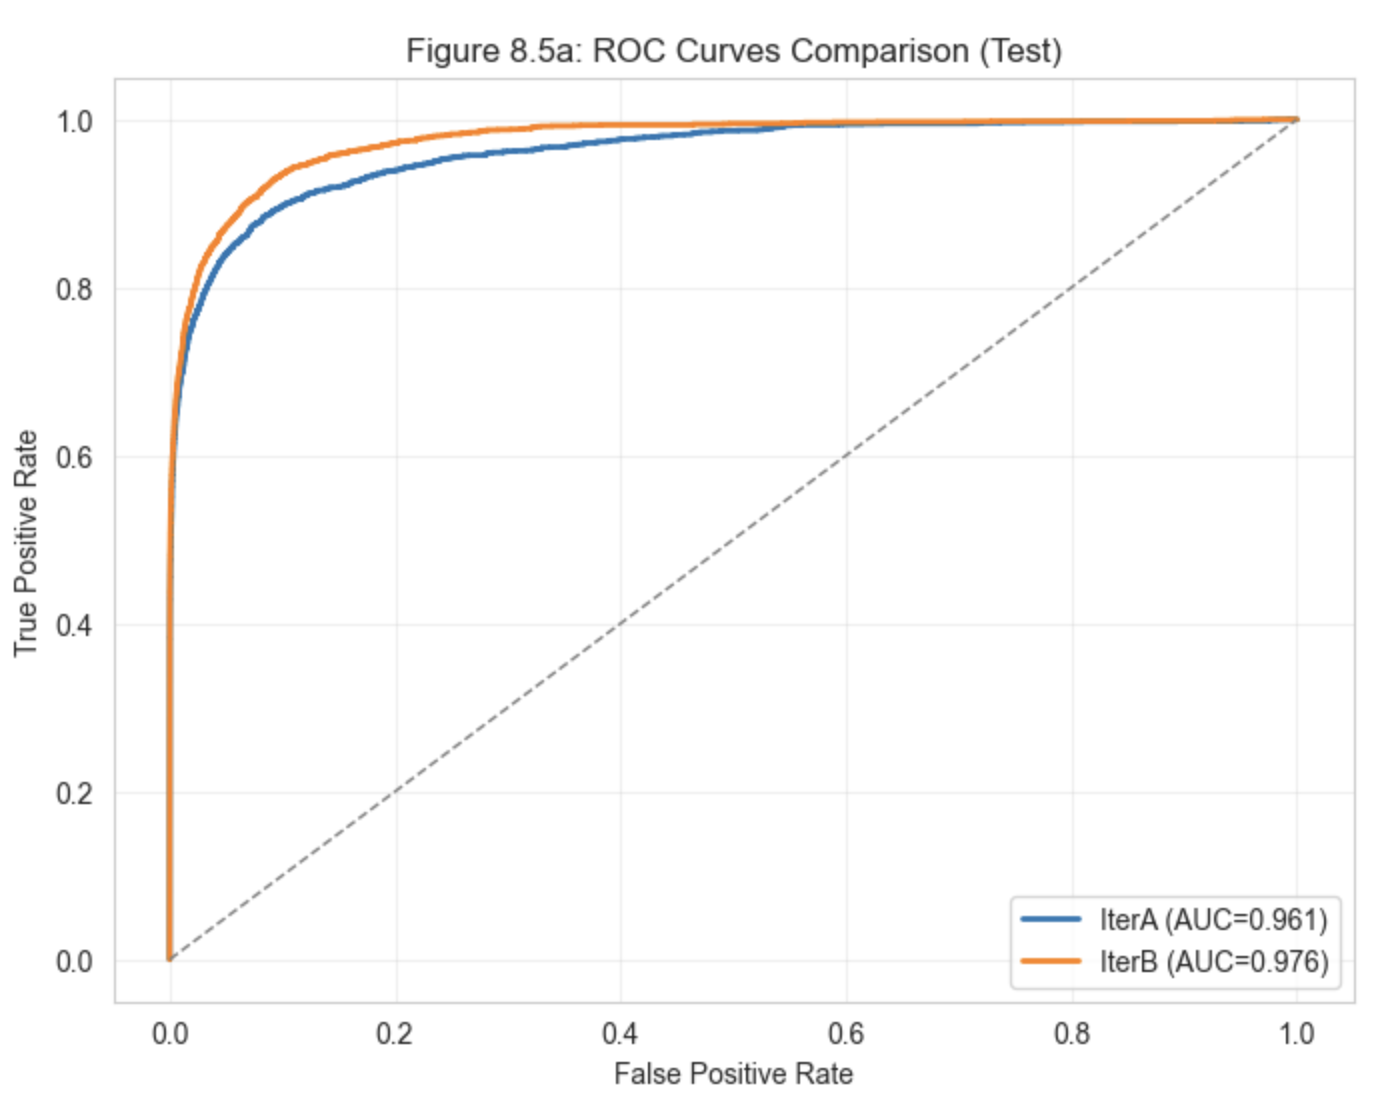
\includegraphics[width=0.9\columnwidth]{8.5a.png}
    \caption{ROC on test set. IterA AUC=0.961; IterB AUC=0.976. Caliber: threshold = $\tau_B$ (determined from validation-set $\tau^*$ and operational constraints); metrics = original-distribution test set (fraud $\approx$ 0.296\%).}
    \label{fig:8.5a}
\end{figure}

\begin{figure}[h!]
    \centering
    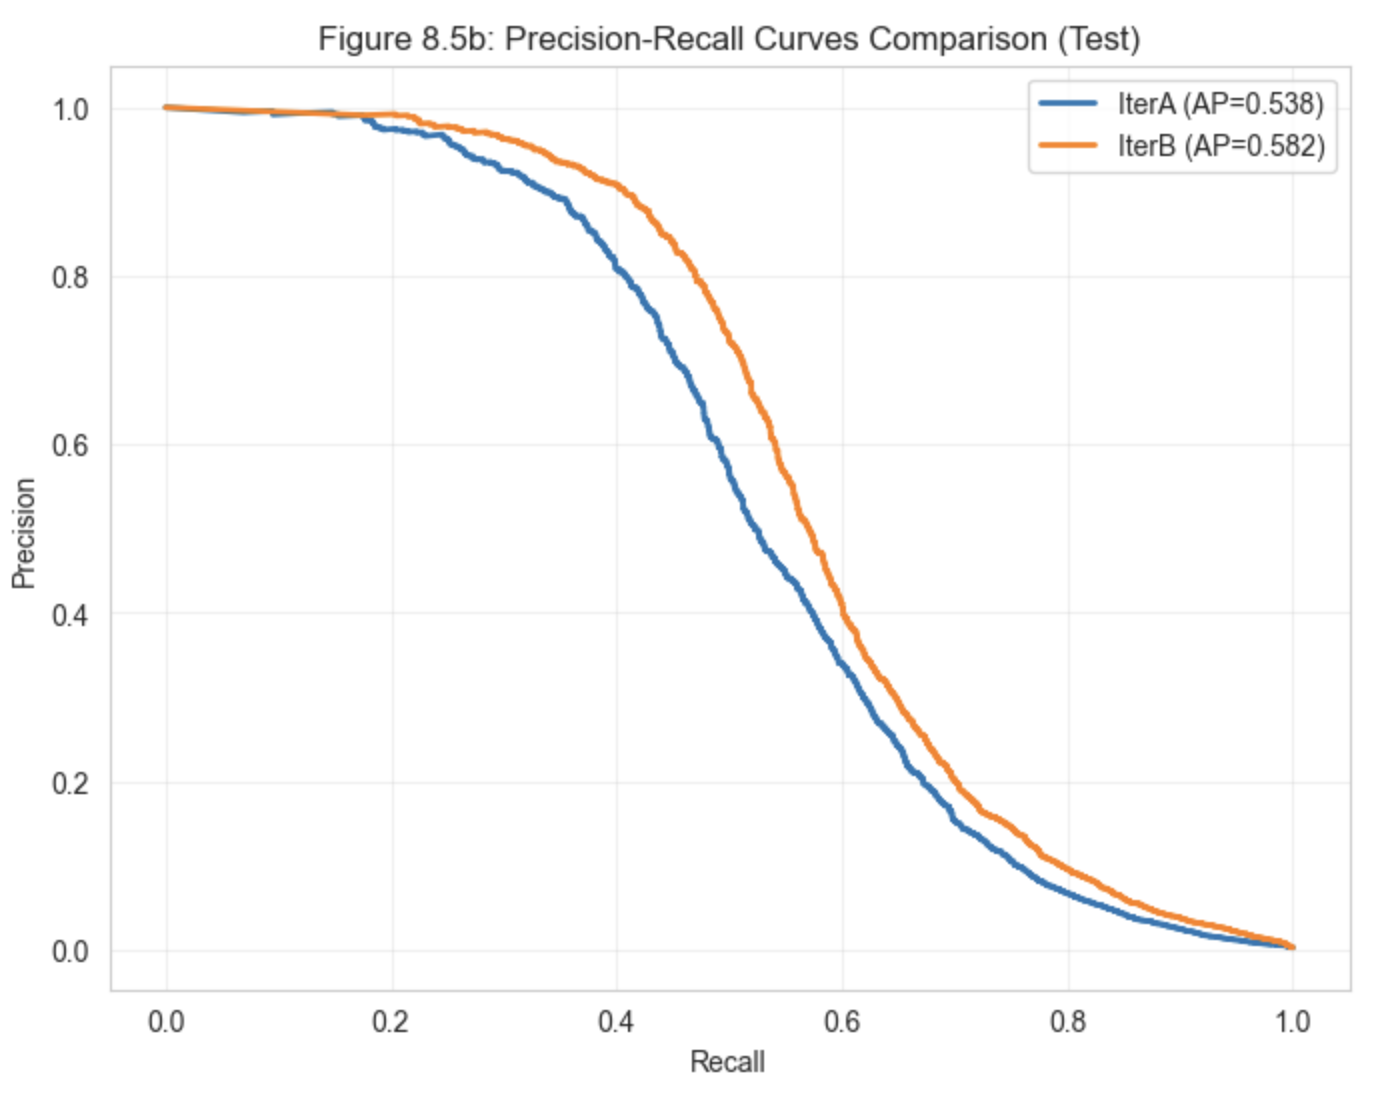
\includegraphics[width=0.9\columnwidth]{8.5b.png}
    \caption{Precision-Recall on test set. IterA AP=0.538; IterB AP=0.582. Caliber: threshold = $\tau_B$ (determined from validation-set $\tau^*$ and operational constraints); metrics = original-distribution test set (fraud $\approx$ 0.296\%).}
    \label{fig:8.5b}
\end{figure}

\begin{figure}[h!]
    \centering
    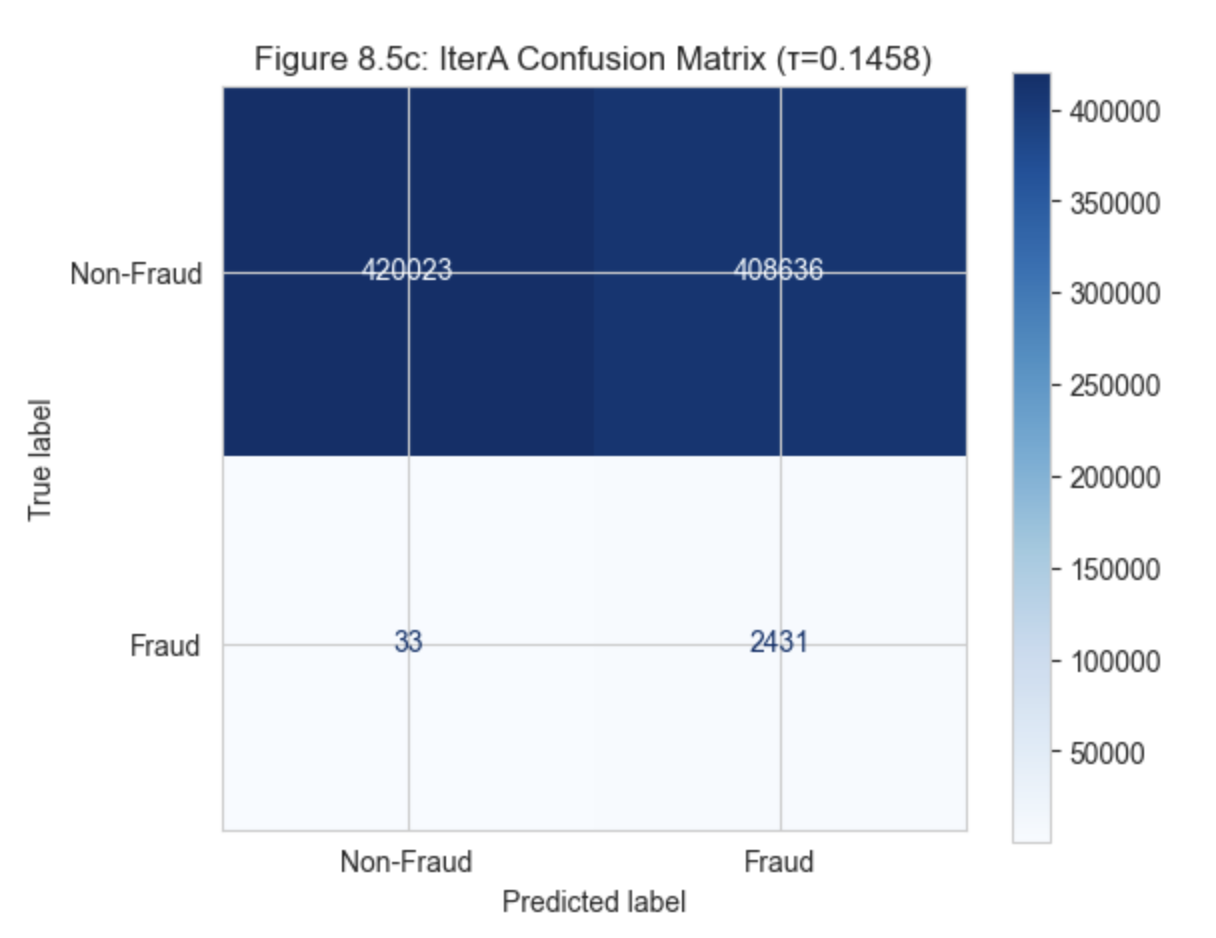
\includegraphics[width=0.9\columnwidth]{8.5c.png}
    \caption{Confusion Matrix on test (IterA, $\tau_B$=0.1458): TN=420,023, FP=408,636, FN=33, TP=2,431. Caliber: threshold = $\tau_B$ (determined from validation-set $\tau^*$ and operational constraints); metrics = original-distribution test set (fraud $\approx$ 0.296\%).}
    \label{fig:8.5c}
\end{figure}

\begin{figure}[h!]
    \centering
    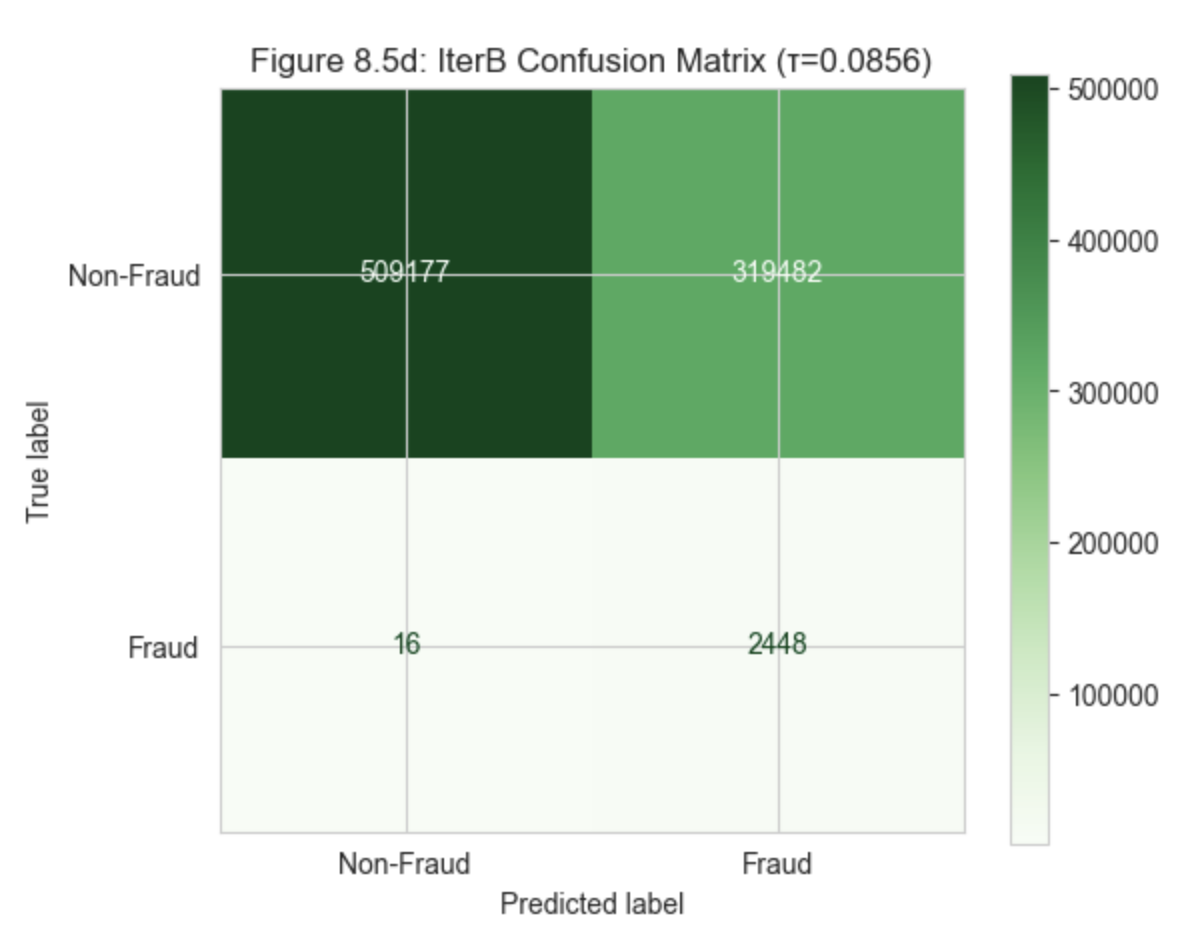
\includegraphics[width=0.9\columnwidth]{8.5d.png}
    \caption{Detailed Performance Metrics Comparison on the Test Set. Caliber: threshold = $\tau_B$ (determined from validation-set $\tau^*$ and operational constraints); metrics = original-distribution test set (fraud $\approx$ 0.296\%).}
    \label{fig:8.5d}
\end{figure}

\textbf{Iteration Results Interpretation and Final Selection}

From the above charts and data, we can draw very clear conclusions:

The two strategies show a vast difference in their raw prediction counts on the test set, which is directly reflected in their respective confusion matrices (see Figure \ref{fig:8.5c}).

1. \textbf{Serious Flaws of IterA (Downsampling)}: Although IterA's recall reaches \textbf{98.7\%}, capturing almost all fraud, this comes at the catastrophic cost of a \textbf{49.3\%} false positive rate (FPR). This means nearly half of normal users would be misclassified as fraudulent, resulting in approximately 492 false alerts per 1000 transactions, with a business cost of \textbf{492.66}, which is completely unacceptable in reality.

2. \textbf{Significant Advantages of IterB (Class Weights)}: In contrast, IterB performs more balanced and excellently across all key metrics. While its recall (66.0\%) is lower than IterA, its precision (27.4\%) is far higher, and the false positive rate (FPR) is controlled at an impressive \textbf{0.52\%}. This directly reflects in business costs: cost per thousand transactions is only \textbf{30.41}, a reduction of \textbf{over 93\%} compared to IterA.

3. \textbf{Model Ranking Ability Comparison (AUC/AP)}: The ROC curves (Figure \ref{fig:8.5a}) and PR curves (Figure \ref{fig:8.5b}) also show that IterB's AUC (0.976 vs 0.961) and AP (0.582 vs 0.538) comprehensively outperform IterA, proving its superior overall discriminative ability and performance on imbalanced data.

\textbf{Conclusion}: Through this iteration comparison, we have proven that \textbf{the class weight method (IterB) is far superior to downsampling (IterA)}. IterB effectively controls false positives and significantly reduces operational costs while maintaining strong fraud detection capability. Therefore, we ultimately select the IterB model. The decision threshold $\tau$*=0.9488 was \textbf{determined on the validation set by minimizing the cost function}, and serves as the final model solution for this data mining project.

This comprehensive comparison validates that thoughtful handling of class imbalance through algorithmic weighting, rather than data manipulation, provides a more practical and cost-effective solution for real-world fraud detection systems.

\bibliographystyle{ACM-Reference-Format}
\bibliography{references}

\bigskip
\noindent\textbf{Disclaimer}\\
\noindent I acknowledge that the submitted work is my own original work in accordance with the University of Auckland guidelines and policies on academic integrity and copyright. (See: \url{https://www.auckland.ac.nz/en/students/forms-policies-and-guidelines/student-policies-and-guidelines/academic-integrity-copyright.html}).

\noindent I also acknowledge that I have appropriate permission to use the data that I have utilised in this project. (For example, if the data belongs to an organisation and the data has not been published in the public domain, then the data must be approved by the rights holder.) This includes permission to upload the data file to Canvas. The University of Auckland bears no responsibility for the student's misuse of data.

\end{document}
\endinput
%%
%% End of file `sample-sigplan.tex'.
